\documentclass[a4paper,12pt]{report}
\usepackage{a4wide}

%\documentclass[a5paper,10pt]{book}
%\usepackage[top=23mm, bottom=18mm, left=15mm, right=25mm]{geometry}
%\geometry{papersize={170mm,220mm}}


\usepackage[utf8x]{inputenc}
\usepackage[danish]{babel}

\usepackage{xr-hyper} %Externe hyper-ref
\usepackage[colorlinks=true, hyperindex=true, linkcolor=minmblaa, citecolor=minmblaa, urlcolor=minmblaa]{hyperref}
\hypersetup{colorlinks=true,filecolor=minmblaa,bookmarksnumbered=true} %Til hyperreferencer. Referencer med farver
\usepackage{needspace} % giver mulighed for at kræve at der skal være et antal tomme linier på siden før ellers indsættes et sideskift.
\usepackage{framed} %Bokse
\usepackage{wrapfig}

\usepackage{amsmath,amsfonts,amssymb,amsthm,mathtools} %Matematikpakker

\setlength{\parindent}{0mm} %Ingen Indhak i første linje i afsnit

\usepackage{color} %Farvepakke

\usepackage{array}
\usepackage{colortbl}
\usepackage{multirow} %Til at flette rækker i tabeller.

\usepackage{verbatim,mhchem}



	% DOWNLOAD FRA: http://sarovar.org/frs/?group_id=52&release_id=97
	% Læg i directory for hoved TEX fil
%\usepackage[draft]{pdfdraftcopy}
%\draftstring{Licens: Kasper Langt Mellemnavn Skårhøj}
%\draftfontsize{30}
	%\draftfontfamily{hlh}
	%\draftangle{45}
	%\definecolor{mycolor}{rgb}{.825,.855,1}
	%\draftcolor{mycolor}
	%\draftfontattrib



% = Sidehoved =
\usepackage{fancyhdr}
\pagestyle{fancy}
\renewcommand{\sectionmark}[1]{\markright{\protect\titlegraphic{dturoed}\textcolor{dtugraa}{\thesection~\MakeUppercase{#1}}}} % \thesection.\
\fancyhead{}
\fancyfoot{}
\fancyhead[R]{\titlefont\thepage}
\fancyhead[C]{}
\fancyhead[L]{\titlefont \small eNote \MakeUppercase{~\thechapter}~\hspace*{1ex}\rightmark}
\renewcommand\headrulewidth{0pt}
\fancypagestyle{plain}{\fancyfoot[C]{}}% {\titlefont\footnotesize\thepage}}
\setlength{\headheight}{15pt}


% = Længder
%\newlength{\envtblsep}\setlength{\envtblsep}{1\FrameSep}
\newlength{\obsl}\setlength{\obsl}{\textwidth-1.2cm-13.2pt}

% Includes:

% =     Fonts (select one)    =
\usepackage{mathpazo}\linespread{1.05} % Palatino needs more leading (space between lines)
\usepackage{bm} % bold math, must be loaded after the fontpackages

% % Til overskrifter
\DeclareTextFontCommand{\th}{\fontencoding{T1}\fontfamily{phv}\fontseries{b}\selectfont}
\newcommand\titlefont{\fontencoding{T1}\fontfamily{phv}\selectfont}


% =     PGF grafik      =
\usepackage{tikz}
\newcommand\titlegraphic[1]{%
\tikz[baseline] %
\draw[thick,color=#1]
(0pt  ,-0.25em) -- (0pt  ,0.85em)
(2.5pt,-0.25em) -- (2.5pt,0.85em)
(5pt  ,-0.25em) -- (5pt  ,0.85em)
(7.5pt,-0.25em) -- (7.5pt,0.85em);\hspace*{0.8ex} %
}

\newcommand\titlegraphicwide[1]{%
\tikz[baseline] %
\draw[line width=0.8mm,color=#1]
(0pt  ,-0.25em) -- (0pt  ,0.85em)
(4.5pt,-0.25em) -- (4.5pt,0.85em)
(9pt  ,-0.25em) -- (9pt  ,0.85em)
(13.5pt,-0.25em) -- (13.5pt,0.85em);\hspace*{0.8ex} %
}


% =      Title Layout      =
\usepackage{titlesec}
\makeatletter
\titleformat{\chapter}
	[display] % Shape
	{\titlefont\Huge\flushleft} % Title and label format
	{\titlefont\LARGE\bfseries \titlegraphicwide{dturoed}\textcolor{dtugraa}{\@chapapp~\thechapter}} % label
	{0.9em} % label/title separation
	{} % before code
	[] % after code
\makeatother
\titleformat{\section}
	[hang] % Shape
	{\titlefont\Large\flushleft} % Title and label format
	{\thesection} % label
	{0.9em} % label/title separation
	{} % before code
	[] % after code
\titleformat{\subsection}
	[hang] % Shape
	{\titlefont\large} % Title and label format
	{\thesubsection} % label
	{0.9em} % label/title separation
	{} % before code
	[] % after code
\titlespacing{\subsection}{0pt}{*6}{*1.5}
\titleformat{\subsubsection}
	[hang] % Shape
	{\titlefont} % Title and label format
	{\thesubsubsection} % label
	{0.9em} % label/title separation
	{} % before code
	[] % after code



% = Farver
\definecolor{dturoed}{rgb}{0.6, 0.0, 0.0}
\definecolor{dtugraa}{rgb}{0.5, 0.5, 0.5}	% Lidt mørkere. Korrekt = 0.4
\definecolor{mingroenstreg}{rgb}{0.4,0.8,0}	% Sekundærfarve 14 : 102/204/0	(Forårsgrøn) -> Eksempler
\definecolor{mingroen}{rgb}{0.32,0.64,0}		% Sekundærfarve 14, 80% mørkere (tekst)
\definecolor{minorangestreg}{rgb}{1,0.6,0}		% Sekundærfarve 1 : 255/153/0	(Orange) -> Opgaver
\definecolor{minorange}{rgb}{0.8,0.48,0}		% Sekundærfarve 1 , 80% mørkere (tekst)

\definecolor{minblaa}{rgb}{0.2,0.4,0.8}	% Sekundærfarve 13 , 51/102/204 	( Blå -> Definitioner etc)
\definecolor{minmblaa}{rgb}{0.16,0.32,0.64}	% Sekundærfarve 13 , 80% mørkere (tekst)
\definecolor{thmbackground}{rgb}{0.97,.97, 0.99}	% Farve 13 - lys baggrund

\definecolor{mingraastreg}{rgb}{.5,.5,.5}
\definecolor{hvadbackground}{rgb}{0.97,.97, 0.97}
\definecolor{sumgul}{rgb}{1,1,.8}

\definecolor{hjmopgfarve}{rgb}{.96,1,.96}


% = Counter
\newcounter{evncount}[chapter]
\setcounter{evncount}{0}
\renewcommand{\theevncount}{\thechapter.\arabic{evncount}}
\renewcommand{\theequation}{\thechapter-\arabic{equation}}


% = Eksempler = example =
\newenvironment{example}[1][]{
	\refstepcounter{evncount}
	\setlength{\obsl}{\textwidth-1.2cm-13.2pt-9pt} % fix width of the info envirnment%
	\def\FrameCommand{ 
		\textcolor{mingroenstreg}{\vrule width 4pt} 
		\hspace{5pt} 
	}%
	\MakeFramed{\advance\hsize-\width \FrameRestore}%
	\needspace{3\baselineskip}
	\titlegraphic{mingroen}
	\textcolor{mingroen}{
		\th{Eksempel \theevncount \hspace*{5mm} #1}
	} 
	\vspace*{3mm}%
	\begin{small}
	\par
}
{
	\end{small}
	\endMakeFramed
}


% = Opgaver = exercise =
\newenvironment{exercise}[1][]{
	\refstepcounter{evncount}
	\setlength{\obsl}{\textwidth-1.2cm-13.2pt-9pt}% fix width of the info envirnment%
	\def\FrameCommand{
		\textcolor{minorangestreg}{\vrule width 4pt}
		\hspace{5pt}
	}%
	\MakeFramed{\advance\hsize-\width \FrameRestore}%
	\needspace{3\baselineskip}
	\titlegraphic{minorange}
	\textcolor{minorange}{
		\th{Opgave \theevncount \hspace*{5mm} #1}
	} 
	\vspace*{3mm}%
	\begin{small}
	\par
}
{
	\end{small}
	\endMakeFramed
}


% = Bevis
\newenvironment{bevis}{
	\setlength{\obsl}{\textwidth-1.2cm-13.2pt-9pt} % fix width of the info envirnment%
	\def\FrameCommand{
		\textcolor{mingraastreg}{\vrule width 4pt} 
		\hspace{5pt}
	}%
	\MakeFramed{\advance\hsize-\width \FrameRestore}%
	\needspace{3\baselineskip}
	\titlegraphic{black}
	\textcolor{black}{
		\th{Bevis}
	}
	\vspace*{3mm}%
	\begin{small}
	\par
}
{
	\bevisslut 
	\end{small}
	\endMakeFramed
}


% = Definition =
\newenvironment{definition}[1][]{
	\vspace{4mm}
	\pagebreak[1]
	\setlength{\obsl}{\textwidth-1.2cm-2\FrameSep-13.2pt}%
	\def\FrameCommand{
		\fboxsep=\FrameSep\fcolorbox{minblaa}{thmbackground}
	}
	\begin{minipage}{\textwidth}
	\MakeFramed{\advance\hsize-\width\FrameRestore}
	\refstepcounter{evncount}
	\titlegraphic{minblaa}
	\textcolor{minmblaa}{
		\th{Definition \theevncount \hspace*{5mm} #1}
	}
	\vspace*{3mm}
	\par
}
{
	\endMakeFramed 
	\end{minipage}
	\vspace{4mm}
}


% = Theorem =
\newenvironment{theorem}[1][]{
	\vspace{4mm}
	\pagebreak[1]%
	\setlength{\obsl}{\textwidth-1.2cm-2\FrameSep-13.2pt}%
	\def\FrameCommand{
		\fboxsep=\FrameSep\fcolorbox{minblaa}{thmbackground}
	}%
	\begin{minipage}{\textwidth}
	\MakeFramed{\advance\hsize-\width\FrameRestore}%
	\refstepcounter{evncount}
	\titlegraphic{minblaa}
	\textcolor{minmblaa}{
		\th{Sætning \theevncount \hspace*{5mm} #1}
	}
	\vspace*{3mm}
	\par
}
{
	\endMakeFramed 
	\end{minipage}
	\vspace{4mm}
}


% = Lemma =
\newenvironment{lemma}[1][]{
	\vspace{4mm}
	\pagebreak[1]
	\setlength{\obsl}{\textwidth-1.2cm-2\FrameSep-13.2pt}%
	\def\FrameCommand{
		\fboxsep=\FrameSep \fcolorbox{minblaa}{thmbackground}
	}
	\begin{minipage}{\textwidth} 
	\MakeFramed{\advance\hsize-\width \FrameRestore}
	\refstepcounter{evncount}
	\titlegraphic{minblaa}
	\textcolor{minmblaa}{
		\th{Hjælpesætning \theevncount \hspace*{5mm} #1}
	}
	\vspace*{3mm}
	\par
}
{
	\endMakeFramed 
	\end{minipage}
	\vspace{4mm}
}


% = Corollary =
\newenvironment{corollary}[1][]{
	\vspace{4mm}
	\pagebreak[1]
	\setlength{\obsl}{\textwidth-1.2cm-2\FrameSep-13.2pt}%
	\def\FrameCommand{
		\fboxsep=\FrameSep \fcolorbox{minblaa}{thmbackground}
	}
	\begin{minipage}{\textwidth} 
	\MakeFramed{\advance\hsize-\width \FrameRestore}
	\refstepcounter{evncount}
	\titlegraphic{minblaa}
	\textcolor{minmblaa}{
		\th{Følgesætning \theevncount \hspace*{5mm} #1}
	}
	\vspace*{3mm}
	\par
}
{
	\endMakeFramed 
	\end{minipage}
	\vspace{4mm}
}


% = Metode = method
\newenvironment{method}[1][]{
	\vspace{4mm}
	\pagebreak[1]
	\setlength{\obsl}{\textwidth-1.2cm-2\FrameSep-13.2pt}%
	\def\FrameCommand{
		\fboxsep=\FrameSep \fcolorbox{black}{hvadbackground}
	}
	\begin{minipage}{\textwidth} 
	\MakeFramed{\advance\hsize-\width \FrameRestore}
	\refstepcounter{evncount}
	\titlegraphic{black}
	\textcolor{black}{
		\th{Metode \theevncount \hspace*{5mm} #1}
	}
	\vspace*{3mm}
	\par
}
{
	\endMakeFramed
	\end{minipage}
	\vspace{4mm}
}


% = Forklaring = explain =
\newenvironment{explain}[1][]{
	\vspace{4mm}
	\pagebreak[1]
	\setlength{\obsl}{\textwidth-1.2cm-2\FrameSep-13.2pt}%
	\def\FrameCommand{
		\fboxsep=\FrameSep \fcolorbox{black}{hvadbackground}
	}
	\MakeFramed{\advance\hsize-\width \FrameRestore}
	\refstepcounter{evncount}
	\titlegraphic{black}
	\textcolor{black}{
		\th{Forklaring \theevncount \hspace*{5mm} #1}
	}
	\vspace*{3mm}
	\par
}
{
	\endMakeFramed
	\vspace{4mm}
}


% = Bemærkning = remark =
\newenvironment{remark}[1][]{
	\vspace{4mm}
	\pagebreak[1]
	\setlength{\obsl}{\textwidth-1.2cm-2\FrameSep-13.2pt}%
	\def\FrameCommand{
		\fboxsep=\FrameSep \fcolorbox{black}{hvadbackground}
	}
	\begin{minipage}{\textwidth} 
	\MakeFramed{\advance\hsize-\width \FrameRestore}
	\refstepcounter{evncount}
	\titlegraphic{black}
	\textcolor{black}{
		\th{Bemærkning \theevncount \hspace*{5mm} #1}
	}
	\vspace*{3mm}
	\par
}
{
	\endMakeFramed 
	\end{minipage}
	\vspace{4mm}
}







% = OBS! = obs =
\newenvironment{obs}{\vspace{4mm}\par%
\begin{tabular}{m{1.2cm}<{\hspace*{2mm}}@{}|m{\obsl}@{}}\hspace*{-4pt}\raggedleft
\includegraphics[width=1.1cm]{../Strukturfiler/FIGS/Alert01} & \begin{minipage}{\obsl}}{\end{minipage}\\ \end{tabular}\vspace{4mm}\par}


% = INFO = info =
\newenvironment{info}{\vspace{4mm}\par%
\begin{tabular}{m{1.2cm}<{\hspace*{2mm}}@{}|m{\obsl}@{}}\hspace*{-4pt}\raggedleft
\includegraphics[width=1.1cm]{../Strukturfiler/FIGS/Info01} & \begin{minipage}{\obsl}}{\end{minipage}\\ \end{tabular}\vspace{4mm}\par}


% = THINK= think =
\newenvironment{think}{\vspace{4mm}\par%
\begin{tabular}{m{1.2cm}<{\hspace*{2mm}}@{}|m{\obsl}@{}}\hspace*{-4pt}\raggedleft
\includegraphics[width=0.7cm]{../Strukturfiler/FIGS/ChessPiece} & \begin{minipage}{\obsl}}{\end{minipage}\\ \end{tabular}\vspace{4mm}\par}


% = AHA= aha =
\newenvironment{aha}{\vspace{4mm}\par%
\begin{tabular}{m{1.2cm}<{\hspace*{2mm}}@{}|m{\obsl}@{}}\hspace*{-4pt}\raggedleft
\includegraphics[width=1.1cm]{../Strukturfiler/FIGS/Think} & \begin{minipage}{\obsl}}{\end{minipage}\\ \end{tabular}\vspace{4mm}\par}


% = BUILDUP= build =
\newenvironment{build}{\vspace{4mm}\par%
\begin{tabular}{m{1.2cm}<{\hspace*{2mm}}@{}|m{\obsl}@{}}\hspace*{-4pt}\raggedleft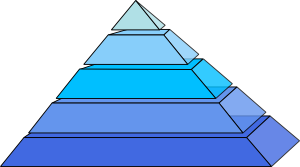
\includegraphics[width=1.1cm]{../Strukturfiler/FIGS/BluePyramid} & \begin{minipage}{\obsl}}{\end{minipage}\\ \end{tabular}\vspace{4mm}\newline}


% = Forudsætning = basis
\newenvironment{basis}{\begin{flushleft} \begin{itshape} }{\end{itshape} \end{flushleft}}


% = Opsummering =
\newenvironment{summary}{\clearpage\pagecolor{sumgul}\section{Opsummering}}{\newpage\pagecolor{white}}











% = Counter
\newcounter{opgavecount}[section]
\setcounter{opgavecount}{0}
\newcounter{spgcount}[opgavecount]
\setcounter{spgcount}{0}
\renewcommand{\thespgcount}{\alph{spgcount})}



% = EXERCISE = (DIVIDER)

\newcommand{\exercisebegin}[1][]{\bigskip\needspace{3\baselineskip}\refstepcounter{opgavecount}\titlegraphic{mingroen}\textcolor{mingroen}{\th{Opgave \theopgavecount \hspace*{1cm} #1}}\medskip\par}

% = QUIZEXERCISE = (DIVIDER)

\newcommand{\quizexercisebegin}[1][]{\bigskip\needspace{3\baselineskip}\refstepcounter{opgavecount}\titlegraphic{mingroen}\textcolor{mingroen}{\th{Quiz-Opgave \theopgavecount \hspace*{1cm} #1}}\medskip\par}

% = QUESTION =

\newenvironment{question}{\refstepcounter{spgcount}\begin{itemize}\item[\thespgcount]}{\end{itemize}\hspace*{\fill}}

% = VINK =

\newenvironment{vink}{\begin{tabular}{m{.9cm}<{\hspace*{2mm}}@{}|m{\obsl}@{}}\hspace*{-4pt}\raggedleft
\includegraphics[width=.9cm]{../Strukturfiler/FIGS/Think} & \begin{minipage}{\obsl}}{\end{minipage}\\ \end{tabular}\medskip\\}
	
% = FACIT =

\newenvironment{facit}{\begin{tabular}{m{.9cm}<{\hspace*{2mm}}@{}|m{\obsl}@{}}\hspace*{-4pt}\raggedleft
\includegraphics[width=.9cm]{../Strukturfiler/FIGS/Check} & \begin{minipage}{\obsl}}{\end{minipage}\\ \end{tabular}\medskip\\}








\newcommand{\afsnit}[1]{\bigskip\th{\titlegraphic{mingroen}\textcolor{mingroen}{#1}} \\ \rule[7pt]{.4\textwidth}{1pt} \vspace*{-2.5mm}\par}

% (DIVIDER):
\newcommand{\ugedagdatotitel}[4]{\pagebreak[4]\section{Semesteruge #1 -- #2 Dag \hspace*{1mm} (#3)} \vspace*{-4mm} \rule[5pt]{\textwidth}{1pt}\vspace*{-2.5mm} \begin{center}\large{\th{#4}}\end{center} \fancyhead[C]{\th{Semesteruge #1}}}

\newenvironment{skema}[1]{\definecolor{shadecolor}{rgb}{0.96,.98, 1.0} \setlength{\FrameSep}{6pt} \renewcommand{\FrameHeightAdjust}{10pt} \vspace*{-4pt}\begin{shaded} \begin{tabular}{#1}}{\end{tabular} \end{shaded} \vspace*{-7pt}}


% ========================

% MAKROER

%\newenvironment{matr}[1][]{\hspace*{-.8mm}\left[\hspace*{-1mm}\begin{array}{#1}}{\end{array}\hspace*{-1mm}\right]\hspace*{-.8mm}}
\newcommand{\bevisslut}{\begin{scriptsize} \begin{flushright} $ \blacksquare $ \end{flushright} \end{scriptsize}}

\newcommand{\tref}[2]{\hyperref[#1]{#2 \ref*{#1}}}
\newcommand{\thref}[2]{\hyperref[#1]{#2}}

\newcommand{\refA}[1]{\colorbox{yellow}{\ref{#1}}}
\newcommand{\hrefA}[2]{\colorbox{yellow}{\href{#1}{#2}}}
\newcommand{\trefA}[2]{\colorbox{yellow}{\hyperref[#1]{#2 \ref*{#1}}}}
\newcommand{\threfA}[2]{\colorbox{yellow}{\hyperref[#1]{#2}}}

\newenvironment{matr}[1]{\hspace*{-.8mm}\begin{bmatrix}\hspace*{-1mm}\begin{array}{#1}}{\end{array}\hspace*{-1mm}\end{bmatrix}\hspace*{-.8mm}}
\newcommand{\transp}{\hspace*{-.6mm}^{\top}}

\newcommand{\maengde}[2]{\left\lbrace \hspace*{-1mm} \begin{array}{c|c} #1 & #2 \end{array} \hspace*{-1mm} \right\rbrace}

\newenvironment{eqnalign}[1]{\setlength{\arraycolsep}{1.3pt}\begin{equation}\begin{array}{#1}}{\end{array}\end{equation}\par}
\newcommand{\eqnl}{\setlength{\arraycolsep}{1.3pt}}

\newcommand{\matind}[3]{{_\mathrm{#1}\mathbf{#2}_\mathrm{#3}}}
\newcommand{\vekind}[2]{{_\mathrm{#1}\mathbf{#2}}}
\newcommand{\jac}[2]{{\mathrm{Jacobi}_\mathbf{#1} (#2)}}
\newcommand{\diver}[2]{{\mathrm{div}\mathbf{#1} (#2)}}
\newcommand{\rot}[1]{{\mathbf{rot}\mathbf{(#1)}}}

\newcommand{\am}{\mathrm{am}}
\newcommand{\gm}{\mathrm{gm}}
\newcommand{\E}{\mathrm{E}}
\newcommand{\Span}{\mathrm{span}}
\newcommand{\mU}{\mathbf{U}}

\newcommand{\ms}{\medskip\\}
\newcommand{\bs}{\bigskip\\}

\newcommand{\mA}{\mathbf{A}}
\newcommand{\mB}{\mathbf{B}}
\newcommand{\mC}{\mathbf{C}}
\newcommand{\mD}{\mathbf{D}}
\newcommand{\mE}{\mathbf{E}}
\newcommand{\mF}{\mathbf{F}}
\newcommand{\mK}{\mathbf{K}}
\newcommand{\mI}{\mathbf{I}}
\newcommand{\mM}{\mathbf{M}}
\newcommand{\mN}{\mathbf{N}}
\newcommand{\mQ}{\mathbf{Q}}
\newcommand{\mT}{\mathbf{T}}
\newcommand{\mV}{\mathbf{V}}
\newcommand{\mW}{\mathbf{W}}
\newcommand{\mX}{\mathbf{X}}
\newcommand{\ma}{\mathbf{a}}
\newcommand{\mb}{\mathbf{b}}
\newcommand{\mc}{\mathbf{c}}
\newcommand{\md}{\mathbf{d}}
\newcommand{\me}{\mathbf{e}}
\newcommand{\mn}{\mathbf{n}}
\newcommand{\mr}{\mathbf{r}}
\newcommand{\mv}{\mathbf{v}}
\newcommand{\mw}{\mathbf{w}}
\newcommand{\mx}{\mathbf{x}}
\newcommand{\mxb}{\mathbf{x_{bet}}}
\newcommand{\my}{\mathbf{y}}
\newcommand{\mz}{\mathbf{z}}
\newcommand{\reel}{\mathbb{R}}
\newcommand{\mL}{\bm{\Lambda}} %Lambda-matrix
\newcommand{\mnul}{\bm{0}}
\newcommand{\trap}[1]{\mathrm{trap}(#1)}
\newcommand{\Det}{\operatorname{Det}}
\newcommand{\adj}{\operatorname{adj}}
\newcommand{\Ar}{\operatorname{Areal}}
\newcommand{\Vol}{\operatorname{Vol}}
\newcommand{\Rum}{\operatorname{Rum}}
\newcommand{\diag}{\operatorname{\bf{diag}}}
\newcommand{\bidiag}{\operatorname{\bf{bidiag}}}
\newcommand{\spanVec}[1]{\mathrm{span}\{#1\}}
\newcommand{\Div}{\operatorname{Div}}
\newcommand{\Rot}{\operatorname{\mathbf{Rot}}}

\newcommand{\Jac}{\operatorname{Jacobi}}
\newcommand{\Tan}{\operatorname{Tan}}
\newcommand{\Ort}{\operatorname{Ort}}
\newcommand{\Flux}{\operatorname{Flux}}
\newcommand{\Cmass}{\operatorname{Cm}}
\newcommand{\Imom}{\operatorname{Im}}
\newcommand{\Pmom}{\operatorname{Pm}}
\newcommand{\IS}{\operatorname{I}}
\newcommand{\IIS}{\operatorname{II}}
\newcommand{\IIIS}{\operatorname{III}}
\newcommand{\Le}{\operatorname{L}}
\newcommand{\app}{\operatorname{app}}
\newcommand{\M}{\operatorname{M}}
\newcommand{\re}{\mathrm{Re}}
\newcommand{\im}{\mathrm{Im}}

\newcommand{\compl}{\mathbb{C}} %de komplekse tal
\newcommand{\e}{\mathrm{e}} %eksponentialfunktionen. lodret 'e', og altså ikke kursiv ligesom andre bogstaver.





% Medialink: SCREEN: (QRcode) + thumbnail image + link på kodenummer (til qr.dtu.dk)
\newcommand{\onlinemedia}[3]{
	\begin{wrapfigure}{r}{3.2cm} 
		\vspace{-30pt} 
		\vspace{#1pt} 
		\begin{flushright} 
			\includegraphics[width=3cm]{qr/#2.png} 
			\tiny 
			\href{http://qr.dtu.dk/#2}{#2: #3}
			\normalsize  
		\end{flushright} 
		\vspace{-10pt} 
	\end{wrapfigure}
}
\newcommand{\onlinemediathumb}[3]{
	\begin{wrapfigure}{r}{3.2cm} 
		\vspace{-30pt} 
		\vspace{#1pt} 
		\begin{flushright} 
			\includegraphics[width=3cm]{qr/#2.png} 
			\includegraphics[width=3cm]{qr/#2_thumb.png} 
			\tiny 
			\href{http://qr.dtu.dk/#2}{#2: #3}
			\normalsize  
		\end{flushright} 
		\vspace{-10pt} 
	\end{wrapfigure}
}



% Index:
\usepackage{makeidx}
\makeindex
\newcommand\ind[2]{\index{#1}\textbf{\textit{\textcolor{black}{#2}}}}

% ###SERVER_EXCLUDE_BEGIN###
\externaldocument[NUID17-]{../../enoten/TN01-Talrum/Talrum}
\externaldocument[NUID1-]{../../enoten/TN02-Ligningssystemer/TNdriver}
\externaldocument[NUID2-]{../../enoten/TN03-Matricer_og_Matrixalgebra/Matricer_og_matrixalgebra}
\externaldocument[NUID3-]{../../enoten/TN04-Kvadratiske_matricer/TNdriver}
\externaldocument[NUID11-]{../../enoten/TN05-Determinanter/Determinanter}
\externaldocument[NUID12-]{../../enoten/TN06-GeometriskeVektorer/GeometriskeVektorer}
\externaldocument[NUID18-]{../../enoten/TN07-Vektorrum/VektorRum}
\externaldocument[NUID21-]{../../enoten/TN08-LinAfbildninger/LinAfbildninger}
\externaldocument[NUID23-]{../../enoten/TN09-Egenvaerdier_og_egenvektorer/TNdriver}
\externaldocument[NUID24-]{../../enoten/TN10-Diagonalisering_med_egenvektorer/TNdriver}
\externaldocument[NUID10-]{../../enoten/TN11-1.ordens_differentialligninger/TNdriver}
\externaldocument[NUID13-]{../../enoten/TN12-1.ordens_differentialligningssystemer/TNdriver}
\externaldocument[NUID14-]{../../enoten/TN13-2.ordens_differentialligninger/TNdriver}
\externaldocument[NUID27-]{../../enoten/TN14-Elemenataere_funktioner/Elementaere_Funktioner}
\externaldocument[NUID28-]{../../enoten/TN15-Funktioner2Variable/Funktioner_To_Variable}
\externaldocument[NUID29-]{../../enoten/TN16-Gradienter_og_Tangentplaner/Gradienter_og_Tangentplaner}
\externaldocument[NUID32-]{../../enoten/TN17-Taylor_formler/Taylor_Formler}
\externaldocument[NUID33-]{../../enoten/TN18-Taylor_2Var/Taylor_2Var}
\externaldocument[NUID34-]{../../enoten/TN19-SymMat/SymmetriskeMatricer}
\externaldocument[NUID35-]{../../enoten/TN20-KegleSnit/Keglesnit}
\externaldocument[NUID36-]{../../enoten/TN21-Riemann_Integral/Riemann_01}
\externaldocument[NUID37-]{../../enoten/TN22-Plan_Int/Plan_Int_01}
\externaldocument[NUID39-]{../../enoten/TN23-Flade_Int/Flade_Rum_Int_01}
\externaldocument[NUID40-]{../../enoten/TN24-Vektorfelter/Vektorfelter_01}
\externaldocument[NUID41-]{../../enoten/TN25-Flux/Flux_02}
\externaldocument[NUID42-]{../../enoten/TN26-Gauss/Gauss_01}
\externaldocument[NUID128-]{../../enoten/TN27-Stokes/Stokes_01}
\externaldocument[NUID43-]{../../enoten/TN29-KomplekseTal/KomplekseTal}

\externaldocument[NUID6-]{../../E-math-opgaver/Opgaver/opgU123}
\externaldocument[NUID19-]{../../E-math-opgaver/Opgaver/opgU45}
\externaldocument[NUID20-]{../../E-math-opgaver/Opgaver/opgU678}
\externaldocument[NUID25-]{../../E-math-opgaver/Opgaver/opgU910SD}
\externaldocument[NUID31-]{../../E-math-opgaver/OpgaverF11-U123/opgF123}
% \externaldocument[NUID9-]{../../E-math-opgaver/Opgaver/Dagsordner E10}
% ###SERVER_EXCLUDE_END###


% Begin document and set alternative chapter title:
\begin{document}
\renewcommand{\chaptername}{eNote}

\setcounter{chapter}{16} %SÆT DETTE TAL TIL 1 MINDRE END DET AKTUELLE TRANSFERNOTE-NUMMER!!
%
%%%%%%%%%%%%%%%%%%%%%%%%%%%%%%%%%%%%%%%%%%%%%
%%%%%%%%%%%%%%%%%%%%%%%%%%%%%%%%%%%%%%%%%%%%%
%%% HERFRA SKAL DU SKRIVE ELLER INDSÆTTE %%%%
%%% DEN FIL DU ØNSKER %%%%%%%%%%%%%%%%%%%%%%%
%%%%%%%%%%%%%%%%%%%%%%%%%%%%%%%%%%%%%%%%%%%%%
%%%%%%%%%%%%%%%%%%%%%%%%%%%%%%%%%%%%%%%%%%%%%

\chapter{Taylor's approksimationsformler for funktioner af én variabel} \label{tn17}

\begin{basis}
 I \tref{NUID27-tn14}{eNote} og \tref{NUID29-tn16}{eNote} er det vist  hvordan funktioner af \'{e}n og to variable kan approksimeres med førstegradspolynomier i ethvert (udviklings-)punkt og at graferne for de approksimerende førstegradspolynomier netop er henholdsvis tangenter og tangentplaner til de tilhørende grafer for funktionerne. I denne eNote vil vi vise, hvordan funktionerne kan approksimeres endnu bedre med polynomier af højere grad. Sådanne approksimationer har enormt mange anvendelser -- det er meget nemmere at regne med polynomier end med andre funktioner, så hvis approksimationen til en funktion er tilstrækkelig god, så kan man bruge og regne videre med det approksimerende polynomium i stedet for funktionen selv og så iøvrigt håbe på, at den fejl man derved begår er tilstrækkelig lille. Men hvad betyder {\emph{tilstrækkelig god}} og {\emph{tilstrækkelig lille}}? Og hvordan afhænger det af graden på det approksimerende polynomium? Det finder du svarene på i denne eNote.
\end{basis}

%%%%%%%%%%%%%%%%%%%%%%%%%%%%%%%%%%%%%%%%%%%%%%%%%%%%%%%%%%%%%
%%%%%%%%%%%%%%%%%%%%%%%%%%%%%%%%%%%%%%%%%%%%%%%%%%%%%%%%%%%%%
%%%%%%%%%%%%%%%%%%%%%%%%%%%%%%%%%%%%%%%%%%%%%%%%%%%%%%%%%%%%%



\section{Højere-ordens afledede} \label{secTaylor1}
Vi vil først se på funktioner $f(x)$ af \'{e}n variabel $x$ i et åbent interval i de reelle tal. Vi vil også antage, at funktionen kan differentieres vilkårligt mange gange, altså at alle de afledede funktioner eksisterer for ethvert $x$ i intervallet: $f'(x_{0})$, $f''(x_{0})$, $f'''(x_{0})$, $f^{(4)}(x_{0})$, $f^{(5)}(x_{0})$, osv. hvor $f^{(4)}(x_{0})$ betyder den $4.$ afledede af $f(x)$ i $x_{0}$. Disse højere afledede skal vi bruge til at konstruere (koefficienterne i) de approksimerende polynomier.

\begin{definition}
Hvis en funktion $f(x)$  kan differentieres vilkårligt mange gange i ethvert punkt $x$ i et givet åbent interval $I$ så siger vi, at funktionen er \ind{glat funktion}{glat} i intervallet $I$.
\end{definition}

\begin{example}[Højere-ordens afledede af nogle elementære funktioner] \label{exampDiffn}
Her er nogle højere-ordens afledede af nogle kendte glatte funktioner:
\begin{equation}
\begin{array}{|c|c|c|c|c|c|}
  \hline
  % after \\: \hline or \cline{col1-col2} \cline{col3-col4} ...
  f(x) & f'(x) & f''(x) & f'''(x) & f^{(4)}(x) & f^{(5)}(x) \\ \hline \hline
  \e^{x} & \e^{x} & \e^{x}& \e^{x}&\e^{x} & \e^{x} \\ \hline
  x^{2} & 2x & 2& 0& 0 & 0 \\ \hline
  x^{3} & 3x^{2}& 6x & 6 & 0 &0 \\ \hline
  x^{4} & 4x^{3}& 12x^{2} & 24x & 24 & 0 \\ \hline
  x^{5} & 5x^{4}& 20x^{3} & 60x^{2} & 120x & 120 \\ \hline
  (x-x_{0})^{5} & 5\cdot(x-x_{0})^{4}& 20\cdot(x-x_{0})^{3} & 60\cdot(x-x_{0})^{2} & 120\cdot(x-x_{0}) & 120 \\ \hline
  \cos(x) & -\sin(x) & -\cos(x) & \sin(x) & \cos(x) & -\sin(x)\\ \hline
  \sin(x) & \cos(x) & -\sin(x) & -\cos(x) & \sin(x) & \cos(x)\\ \hline
  \cosh(x) & \sinh(x) &  \cosh(x) & \sinh(x)&  \cosh(x) & \sinh(x)\\ \hline
  \sinh(x) &  \cosh(x) & \sinh(x)&  \cosh(x) & \sinh(x)& \cosh(x) \\ \hline
  \hline
\end{array}
\end{equation}
\end{example}

\begin{aha}
Læg mærke til, at
\begin{enumerate}
\item Den $n$'te afledede $f^{(n)}(x)$ af funktionen $f(x) = (x-x_{0})^{n}$ er
\begin{equation}
f^{(n)}(x) = n\cdot(n-1)\cdot(n-2) \cdots 2\cdot 1 = n!\, \quad ,
\end{equation}
hvor $n!$ ($n$ fakultet) er den korte skrivemåde for produktet af heltallene fra og med $1$ til og med $n$, jævnfør tabel \ref{exampDiffn}, hvor $n!$ optræder med $2! =2$, $3! =6$, $4! =24$, $5! =120$.
\item Ved gentagen differentiation af $\cos(x)$ fås det  samme ''sæt'' af funktioner periodisk med perioden $4$: Hvis $f(x) = \cos(x)$, så er
\begin{equation}
f^{(p)}(x) = f^{(p+4)}(x) \quad \textrm{for alle $p \geq 1$} \quad .
\end{equation}
Det samme gælder for $f(x) = \sin(x)$.
\item Ved gentagen differentiation af den hyperbolske cosinusfunktion $\cosh(x)$ fås igen det samme ''sæt'' af funktioner periodisk med perioden $2$: Hvis $f(x) = \cosh(x)$ fås
\begin{equation}
f^{(p)}(x) = f^{(p+2)}(x) \quad \textrm{for alle $p \geq 1$} \quad .
\end{equation}
Det samme gælder for den hyperbolske sinusfunktion $f(x) = \sinh(x)$.
\end{enumerate}
\end{aha}

\begin{example}[De afledede af en knap så elementær funktion] \label{exampElemInt}
En funktion $f(x)$ kan eksempelvis være givet ved et integral (som i dette tilfælde ikke kan udtrykkes ved de sædvanlige elementære funktioner):
\begin{equation}
f(x) = \int_{0}^{x}\, \e^{-t^{2}}\, dt \quad .
\end{equation}
Men vi kan sagtens differentiere og finde de højere afledede af funktionen for ethvert $x$:
\begin{equation}
f'(x) = \e^{-x^{2}}\quad , \quad f''(x)= -2\cdot x \cdot \e^{-x^{2}}\quad , \quad f'''(x) =  -2 \cdot \e^{-x^{2}} + 4\cdot x^{2}\cdot\e^{-x^{2}}  \quad  \textrm{osv.}
\end{equation}
\end{example}

\begin{example}[De afledede af en ukendt funktion] \label{exampElemDiff}
Vi antager at en funktion $f(x)$ er givet som løsning til en differentialligning med begyndelsesbetingelser i $x_{0}$:
\begin{equation} \label{eqDifflign}
f''(x) + 3f'(x) + 7f(x) = q(x) \quad , \quad \textrm{hvor} \quad f(x_{0}) = 1 \quad , \quad \textrm{og} \quad f'(x_{0}) = -3
\end{equation}
hvor $q(x)$ er en given glat funktion af $x$.
Vi kan igen rimelig let finde de højere afledede af funktionen i $x_{0}$ ved at benytte begyndelsesbetingelserne direkte og ved at {\emph{differentiere differentialligningen}}. Følgende fås fra begyndelsesbetingelserne og fra differentialligningen selv:
\begin{equation}
f'(x_{0}) = -3\quad , \quad f''(x_{0})= q(x_{0}) - 3f'(x_{0}) - 7f(x_{0}) = q(x_{0}) + 2 \quad .
\end{equation}
Den tredje (og de højere) afledede af $f(x)$ fås derefter ved at differentiere begge sider af differentialligningen. F.eks. får vi ved at differentiere \'{e}n gang:
\begin{equation}
f'''(x) + 3f''(x) + 7f'(x) = q'(x)\quad ,
\end{equation}
hvoraf vi får:
\begin{equation}
\begin{aligned}
f'''(x_{0}) &= q'(x_{0}) - 3f''(x_{0}) - 7f'(x_{0}) \\
&= q'(x_{0}) - 3\cdot(q(x_{0}) + 2) - 7\cdot(-3) \\
&= q'(x_{0}) - 3q(x_{0}) +15 \quad .
\end{aligned}
\end{equation}
\end{example}

\section{Approksimation med polynomier}

Ideen med det følgende går nu ud på at finde det polynomium, f.eks. det andengrads-polynomium, som bedst approksimerer en given glat funktion $f(x)$ i og omkring et givet $x_{0}$ i funktionens definitionsmængde $\mathcal{D}m(f)$. \\

Vi prøver derfor at skrive $f(x)$  på følgende måde:
\begin{equation}
f(x) = a_{0} + a_{1}\cdot(x-x_{0}) + a_{2}\cdot(x-x_{0})^{2} + R_{2, x_{0}}(x) \quad ,
\end{equation}
hvor $a_{0}$, $a_{1}$, og $a_{2}$ er passende konstanter der skal vælges således at \ind{restfunktionen}{restfunktionen}
$R_{2, x_{0}}(x)$ er så lille som muligt i og omkring $x_{0}$. Restfunktionen kan vi udtrykke ved $f(x)$ og det polynomium, som vi afprøver:
\begin{equation}
R_{2, x_{0}}(x) = f(x) - a_{0} - a_{1}\cdot(x-x_{0}) - a_{2}\cdot(x-x_{0})^{2} \quad,
\end{equation}
og det er denne funktion, der skal være så tæt på at være $0$ som muligt når $x$ er tæt på $x_{0}$ sådan at forskellen mellem funktionen $f(x)$ og andengradspolynomiet bliver så lille som muligt -- i det mindste tæt på $x_{0}$.\\

Det første naturlige krav er derfor at:
\begin{equation}
R_{2, x_{0}}(x_{0}) = 0 \quad \textrm{svarende til at} \quad f(x_{0}) = a_{0} \quad ,
\end{equation}
hvorved $a_{0}$ nu er bestemt. \\

Det næste naturlige krav, er at grafen for restfunktionen har vandret tangent i $x_{0}$ således at tangenten til restfunktionen derefter er identisk med $x$ aksen:
\begin{equation}
R_{2, x_{0}}'(x_{0}) = 0 \quad \textrm{sådan at} \quad f'(x_{0}) = a_{1} \quad ,
\end{equation}
hvorved $a_{1}$ er bestemt. \\


Det næste krav til restfunktionen er derefter:
\begin{equation}
R_{2, x_{0}}''(x_{0}) = 0 \quad \textrm{svarende til at} \quad f''(x_{0}) = 2\cdot a_{2} \quad ,
\end{equation}
hvorved også $a_{2} = \frac{1}{2}f''(x_{0})$ dermed er bestemt og fastlagt.\\

Vi har dermed fundet
\begin{equation}
f(x) = f(x_{0}) + \frac{f'(x_{0})}{1!}\cdot(x-x_{0}) + \frac{f''(x_{0})}{2!}\cdot(x-x_{0})^{2} + R_{2, x_{0}}(x)
\end{equation}
hvor restfunktionen $R_{2, x_{0}}(x)$ tilfredsstiller følgende krav som gør den meget lille omkring $x_{0}$:
\begin{equation}
R_{2, x_{0}}(x_{0}) = R_{2, x_{0}}'(x_{0}) = R_{2, x_{0}}''(x_{0}) = 0 \quad.
\end{equation}

Hvis vi på tilsvarende måde havde ønsket at finde et approksimerende $n$'te grads polynomium for den samme funktion $f(x)$ havde vi fundet:
\begin{equation}
f(x) = f(x_{0}) + \frac{f'(x_{0})}{1!}\cdot(x-x_{0}) + \cdots +
\frac{f^{(n)}(x_{0})}{n!}\cdot(x-x_{0})^{n} + R_{n, x_{0}}(x) \quad,
\end{equation}
hvor restfunktionen $R_{n, x_{0}}(x)$ er en glat funktion der tilfredsstiller alle kravene:
\begin{equation} \label{eqRestfkt}
R_{n, x_{0}}(x_{0}) = R_{n, x_{0}}'(x_{0}) = \cdots = R_{n, x_{0}}^{(n)}(x_{0})= 0 \quad.
\end{equation}

Det er herefter rimeligt at forvente, dels at disse krav til restfunktionen kan opfyldes og dels at de tilsammen betyder, at restfunktionen selv må 'ligne' og være lige så lille som en potens
af $(x-x_{0})$ tæt ved $x_{0}$. \\

Det er præcis indholdet af følgende hjælpesætning:

\begin{lemma}[Restfunktioner]
Restfunktionen $R_{n, x_{0}}(x)$  kan udtrykkes ud fra $f(x)$  på to ret forskellige måder, og vi skal benytte dem begge i det følgende:
\begin{equation} \label{eqTaylorRestXi}
R_{n, x_{0}}(x) =  \frac{f^{(n+1)}(\xi(x))}{(n+1)!}\cdot(x-x_{0})^{n+1} \quad,
\end{equation}
hvor $\xi(x)$ ligger imellem $x$ og $x_{0}$ i intervallet $I$.\\

  Den anden fremstilling er følgende som indeholder en epsilonfunktion:
\begin{equation} \label{eqTaylorRestEps}
R_{n, x_{0}}(x) =  (x-x_{0})^{n}\cdot \varepsilon_{f}(x-x_{0}) \quad,
\end{equation}
hvor $\varepsilon_{f}(x-x_{0})$ er en epsilonfunktion af $(x-x_{0})$.
\end{lemma}
\begin{bevis}
Vi vil nøjes med at indse den første påstand (\ref{eqTaylorRestXi}) i det allersimpleste tilfælde, nemlig for $n=0$, dvs. følgende: I intervallet mellem (et fastholdt) $x$ og $x_{0}$ findes altid en værdi $\xi$ således at følgende gælder:
\begin{equation}
R_{0, x_{0}}(x) =  f(x) - f(x_{0}) = \frac{f'(\xi)}{(1)!}\cdot(x-x_{0}) \quad.
\end{equation}
Men dette er blot en iklædning af \ind{middelværdisætningen}{middelværdisætningen}: Hvis en glat funktion har værdierne henholdsvis $f(a)$  og $f(b)$ i endepunkterne af et interval $[a, b]$, så har grafen for $f(x)$ et sted en tangent som er parallel med det linjestykke der forbinder de to punkter  $(a, f(a))$ og  $(b, f(b))$, se figur \ref{figMeanVal}.\\

Den anden fremstilling (\ref{eqTaylorRestEps}) følger af den første (\ref{eqTaylorRestXi}) ved  at observere, at
$\frac{f^{(n+1)}(\xi)}{(n+1)!}\cdot(x-x_{0})^{n+1}$ er en epsilonfunktion af $(x-x_{0})$, da $\frac{f^{(n+1)}(\xi)}{(n+1)!}$ er begrænset og da $(x-x_{0})^{n+1}$ selv er en epsilonfunktion.
\end{bevis}

\begin{figure}[ht]
\centerline{ 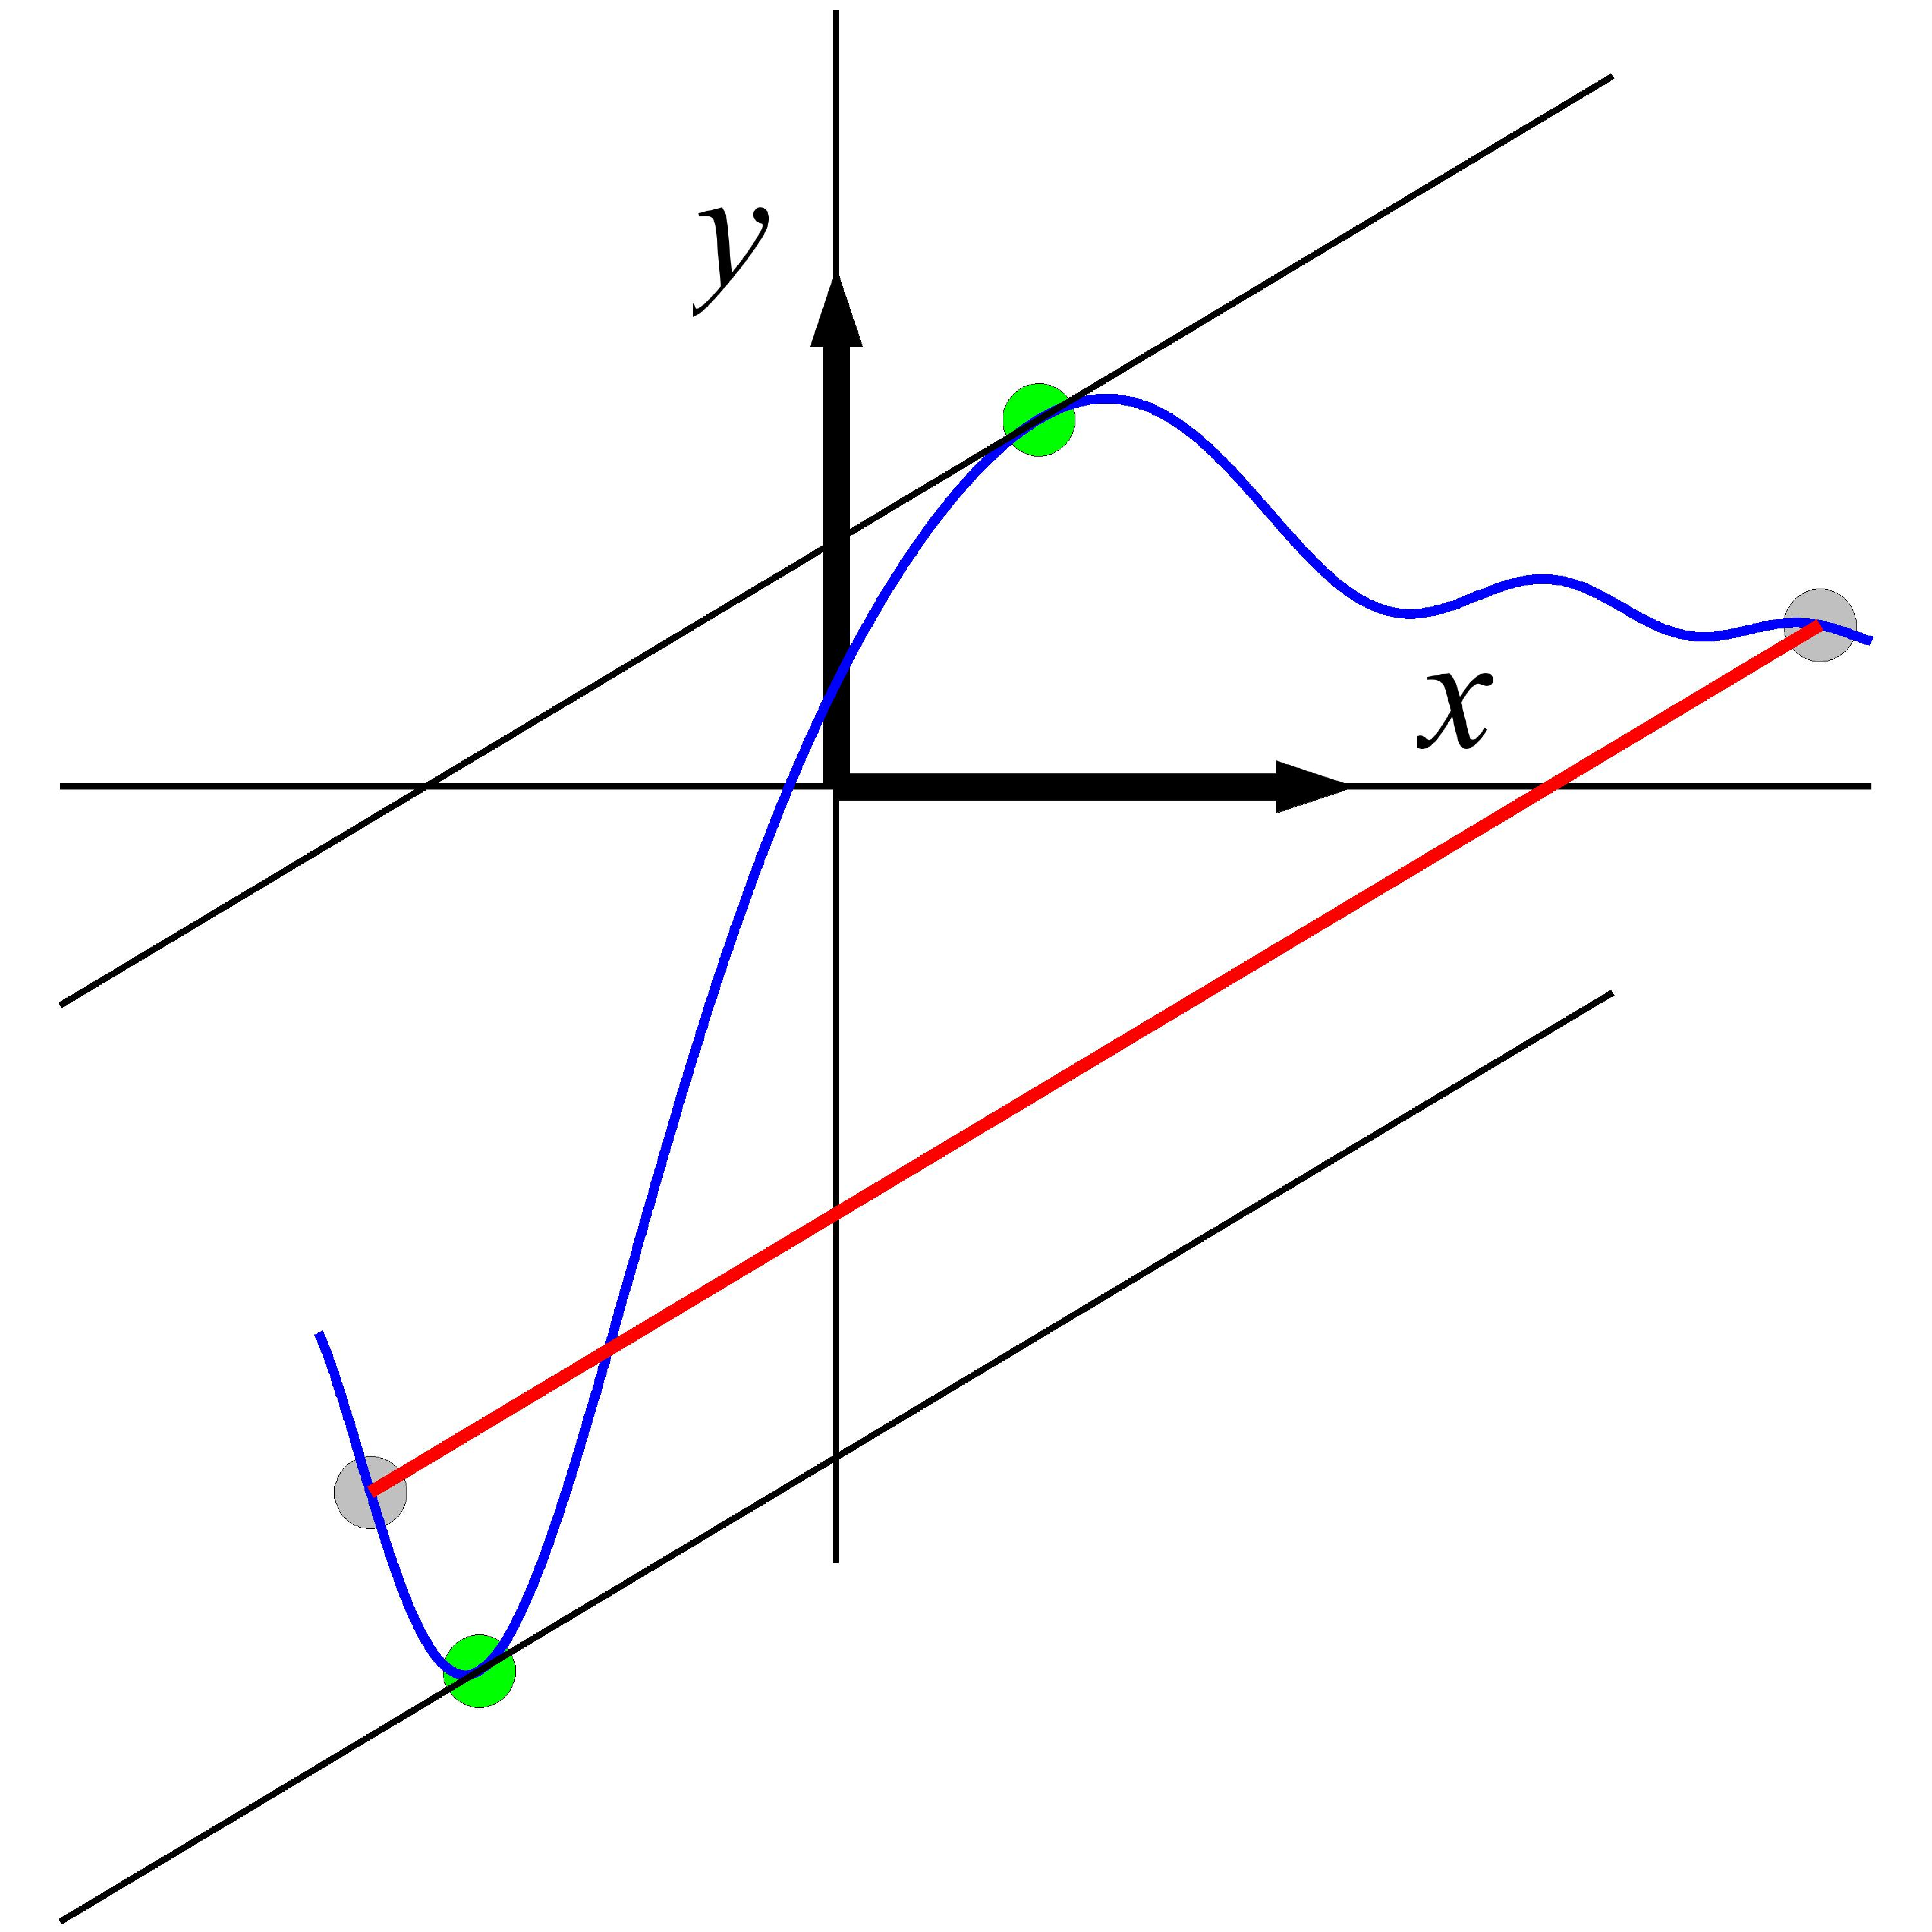
\includegraphics[height=65mm]{plotMeanVal.pdf}}
\begin{center}
\caption{To punkter på den blå graf-kurve for en funktion forbindes med et linjestykke (rød). Middelværdisætningen siger så,
at der findes mindst \'{e}t sted (i det viste tilfælde præcis to steder, markeret med grønt) på kurven mellem de givne punkter hvor hældningskoefficienten $f'(x)$ for tangenten (sort) til kurven er præcis den samme som hældningskoefficienten for det rette linjestykke.} \label{figMeanVal}
\end{center}
\end{figure}

\begin{definition}[Approksimerende polynomium]
Lad $f(x)$ betegne en glat funktion i et interval $I$.
Polynomiet
\begin{equation}
P_{n, x_{0}}(x) = f(x_{0}) + \frac{f'(x_{0})}{1!}\cdot(x-x_{0}) + \cdots +
\frac{f^{(n)}(x_{0})}{n!}\cdot(x-x_{0})^{n}
\end{equation}
kaldes det \ind{approksimerende polynomium}{approksimerende polynomium} af $n$'te grad for funktionen $f(x)$ med udviklingspunkt $x_{0}$.
\end{definition}

Opsamlende har vi derfor:

\begin{theorem}[Taylor's formler]
Enhver glat funktion $f(x)$ kan  for ethvert $n$ opdeles i et approksimerende polynomium af grad $n$ og en restfunktion således:
\begin{equation}
f(x) = P_{n, x_{0}}(x) + R_{n, x_{0}}(x) \quad ,
\end{equation}
hvor restfunktionen kan udtrykkes på følgende måder:
\begin{equation} \label{eqRestfunk}
\begin{aligned}
R_{n, x_{0}}(x) &=  \frac{f^{(n+1)}(\xi(x))}{(n+1)!}\cdot(x-x_{0})^{n+1} \quad \textrm{for et $\xi(x)$ mellem $x$ og $x_{0}$} \\
\textrm{og} \\
R_{n, x_{0}}(x) &=  (x-x_{0})^{n}\cdot \varepsilon_{f}(x-x_{0}) \quad .
\end{aligned}
\end{equation}
\end{theorem}





Det er især Taylor's grænseformel (hvor restfunktionen udtrykkes med en epsilonfunktion) vi vil gøre brug af i det følgende. Vi nævner den version eksplicit:

\begin{theorem}[Taylor's grænseformel]
Lad $f(x)$ betegne en glat funktion i et åbent interval $I$ som indeholder et givet $x_{0}$.
Så gælder der for alle $x$ i intervallet og for ethvert helt tal $n \geq 0$ følgende
\begin{equation*}
f(x) = f(x_{0}) + \frac{f'(x_{0})}{1!}\cdot(x-x_{0}) + \cdots +
\frac{f^{(n)}(x_{0})}{n!}\cdot(x-x_{0})^{n} + (x-x_{0})^{n}\cdot\varepsilon_{f}(x-x_{0}) \quad ,
\end{equation*}
hvor $\varepsilon_{f}(x-x_{0})$ betegner en epsilonfunktion af $(x-x_{0})$, dvs. $\varepsilon_{f}(x-x_{0}) \to 0 $ for $x \to x_{0}$.
\end{theorem}

\begin{example}[Et polynomiums approksimerende polynomier] \label{exampPolyApproks}
Man kunne forledes til at tro, at ethvert polynomium er sit eget approksimerende polynomium fordi ethvert polynomium må da være den bedste approksimation til sig selv.
Her er et eksempel der viser, at det ikke er {\emph{så}} simpelt. Vi ser på tredjegradspolynomiet
\begin{equation}
f(x) = 1 + x + x^{2} + x^{3} \quad .
\end{equation}
Polynomiet $f(x)$ har følgende ret forskellige approksimerende polynomier - i afhængighed af valg af {\emph{udviklingspunkt}} $x_{0}$ og {\emph{udviklingsgrad}} $n$:
\begin{equation}
\begin{aligned}
P_{7, x_{0}=0}(x) &= 1 + x + x^{2} + x^{3} \\
P_{3, x_{0}=0}(x) &= 1 + x + x^{2} + x^{3} \\
P_{2, x_{0}=0}(x) &= 1 + x + x^{2}  \\
P_{1, x_{0}=0}(x) &= 1 + x   \\
P_{0, x_{0}=0}(x) &= 1  \\
P_{7, x_{0}=1}(x) &= 1 + x + x^{2} + x^{3} \\
P_{3, x_{0}=1}(x) &= 1 + x + x^{2} + x^{3} \\
P_{2, x_{0}=1}(x) &=  2 - 2\cdot x + 4\cdot x^{2}\\
P_{1, x_{0}=1}(x) &=  -2 + 6\cdot x\\
P_{0, x_{0}=1}(x) &= 4 \\
P_{7, x_{0}=7}(x) &= 1 + x + x^{2} + x^{3} \\
P_{3, x_{0}=7}(x) &= 1 + x + x^{2} + x^{3}\\
P_{2, x_{0}=7}(x) &= 344 - 146\cdot x + 22\cdot x^{2}\\
P_{1, x_{0}=7}(x) &= -734 + 162\cdot x\\
P_{0, x_{0}=7}(x) &= 400 \quad .
\end{aligned}
\end{equation}
\end{example}


\begin{exercise}[Rest-funktioner for polynomier]
For funktionen $f(x) =  1 + x + x^{2} + x^{3}$ betragtes følgende to opdelinger i approksimerende polynomier og tilhørende restfunktioner:
\begin{equation}
\begin{aligned}
f(x) &= P_{2, x_{0}=1}(x) + R_{2, x_{0}=1}(x) \quad \textrm{og} \\ \\
f(x) &= P_{1, x_{0}=7}(x) + R_{1, x_{0}=7}(x) \quad,
\end{aligned}
\end{equation}
hvor de to approksimerende polynomier  $P_{2, x_{0}=1}(x)$ og $P_{1, x_{0}=7}(x)$ allerede er angivet i eksempel \ref{exampPolyApproks}. Bestem de to restfunktioner $R_{2, x_{0}=1}(x)$ og $R_{1, x_{0}=7}(x)$ udtrykt på begge de to måder som er vist i  \ref{eqRestfunk}: For hver af de to  restfunktioner angives de respektive udtryk for $\xi(x)$ og for $\varepsilon(x-x_{0})$.
\end{exercise}




\begin{example}[Taylor's grænseformel med udviklingspunkt $x_{0}=0$]\label{exampTaylorGraens}
Her er nogle ofte benyttede funktioner med deres respektive approksimerende polynomier (og tilhørende restfunktioner udtrykt med epsilonfunktioner) med det fælles udviklingspunkt $x_{0}=0$ og vilkårlig høj grad:
\begin{equation}
\begin{aligned}
\e^{x} &= 1 + x + \frac{x^{2}}{2!} + \cdots + \frac{x^{n}}{n!} + x^{n}\cdot\varepsilon(x) \\
\e^{x^{2}} &= 1 + x^{2} + \frac{x^{4}}{2!} + \cdots + \frac{x^{2n}}{n!} + x^{2n}\cdot\varepsilon(x) \\
\cos(x) &= 1 - \frac{x^{2}}{2!} + \frac{x^{4}}{4!} + \cdots + (-1)^{n}\cdot\frac{x^{2n}}{(2n)!} + x^{2n}\cdot\varepsilon(x) \\
\sin(x) &= x - \frac{x^{3}}{3!} +  \frac{x^{5}}{5!}+ \cdots + (-1)^{n}\cdot\frac{x^{2n+1}}{(2n+1)!} + x^{2n+1}\cdot\varepsilon(x)\\
\ln(1+x) &= x - \frac{x^{2}}{2} + \cdots + (-1)^{n-1}\cdot\frac{x^{n}}{n!} + x^{n}\cdot\varepsilon(x) \\
\ln(1-x) &= -x - \frac{x^{2}}{2} - \cdots - \frac{x^{n}}{n!} - x^{n}\cdot\varepsilon(x) \\
\frac{1}{1+x} &= 1 - x +x^{2} - x^{3} + \cdots + (-1)^{n-1}\cdot x^{n-1} + x^{n}\cdot\varepsilon(x) \\
\frac{1}{1-x} &= 1 + x +x^{2} + x^{3} + \cdots +  x^{n-1} + x^{n}\cdot\varepsilon(x)
\end{aligned}
\end{equation}
\end{example}


\begin{aha}
Bemærk, at der i Taylor's grænseformel altid afsluttes med en epsilon-funktion og med en potens af $x$ der er præcis den samme som den sidste potens der benyttes i det foranstående approksimerende polynomium.
\end{aha}


\section{Kontinuerte udvidelser} \label{secKontUdvid}
Funktionen $f(x) = \sin(x)/x$ er ikke defineret i $x=0$. Vi vil undersøge, om vi kan udvide funktionen til at have en værdi i $0$, således at den udvidede funktion er kontinuert i $0$. Dvs. vi vil finde en værdi $a$, således at $a$-udvidelsen
\begin{equation}
\widetilde{f} = \left\{
        \begin{array}{ll}
         \frac{\sin(x)}{x} \, \,  & \hbox{for} \quad x \neq 0 \\
          a \, \, & \hbox{for} \quad x = 0
        \end{array}
      \right.
\end{equation}
er kontinuert i $x=0$, dvs. således at
\begin{equation}
 \frac{\sin(x)}{x} \to a \quad \textrm{for} \quad  x \to 0 \quad.
\end{equation}


En direkte anvendelse af Taylor's grænseformel optræder ved bestemmelse af grænseværdier for sådanne brøker $f(x)/g(x)$ hvor begge funktionerne,
altså tælleren $f(x)$ og nævneren $g(x)$, går imod $0$ for $x$ gående imod $0$. Hvad sker der med brøken når $x$ går imod $0$? Vi illustrerer  med en række eksempler. Bemærk, at selv om tæller-funktionen og nævner-funktionen begge er kontinuerte i $0$, så behøver brøken ikke selv at være det.

\begin{example}[Grænseværdier for funktionsbrøker] \label{exampFunkFrac}
\begin{equation}
\frac{\sin(x)}{x} = \frac{x + x^{1}\cdot\varepsilon(x)}{x} = 1 + \varepsilon(x) \to 1 \quad \textrm{for} \quad x \to 0 \quad .
\end{equation}

\begin{equation}
\frac{\sin(x)}{x^{2}} = \frac{x - \frac{1}{3!}x^{3} + x^{3}\cdot\varepsilon(x)}{x^{2}} = \frac{1}{x} - \frac{x}{3!} + x\cdot \varepsilon(x) \quad,
\end{equation}
som ikke har nogen grænseværdi for $x \to 0$. Derfor findes der ikke nogen kontinuert udvidelse i dette tilfælde.

\begin{equation}
\frac{\sin(x^2)}{x^{2}} \to 1 \quad \textrm{for} \quad x \to 0 \quad \textrm{fordi} \quad \frac{\sin(u)}{u} \to 1 \quad \textrm{for} \quad u \to 0 \quad.
\end{equation}

\begin{equation}
\frac{\sin(x)-x}{x^{2}} = \frac{x - \frac{1}{3!}x^{3} + x^{3}\cdot\varepsilon(x) - x}{x^{2}} = - \frac{x}{3!} + x\cdot \varepsilon(x) \to 0 \quad \textrm{for} \quad x \to 0 \quad .
\end{equation}

\begin{equation}
\frac{\sin(x)-x}{x^{3}} =   \frac{x - \frac{1}{3!}x^{3} + x^{3}\cdot\varepsilon(x) - x}{x^{3}} = - \frac{1}{3!} + \cdot \varepsilon(x)                                     \to -\frac{1}{6} \quad \textrm{for} \quad x \to 0 \quad .
\end{equation}
\end{example}


\begin{aha}
Ved bestemmelse af sådanne grænseværdier udvikles de approksimerende polynomier i tæller og nævner til så høje grader at grænseværdien ''fremkommer'' ved division i tæller og nævner med en potens af $x$.
\end{aha}

 Her er et lidt mere kompliceret eksempel:


\begin{figure}[ht]
\centerline{ 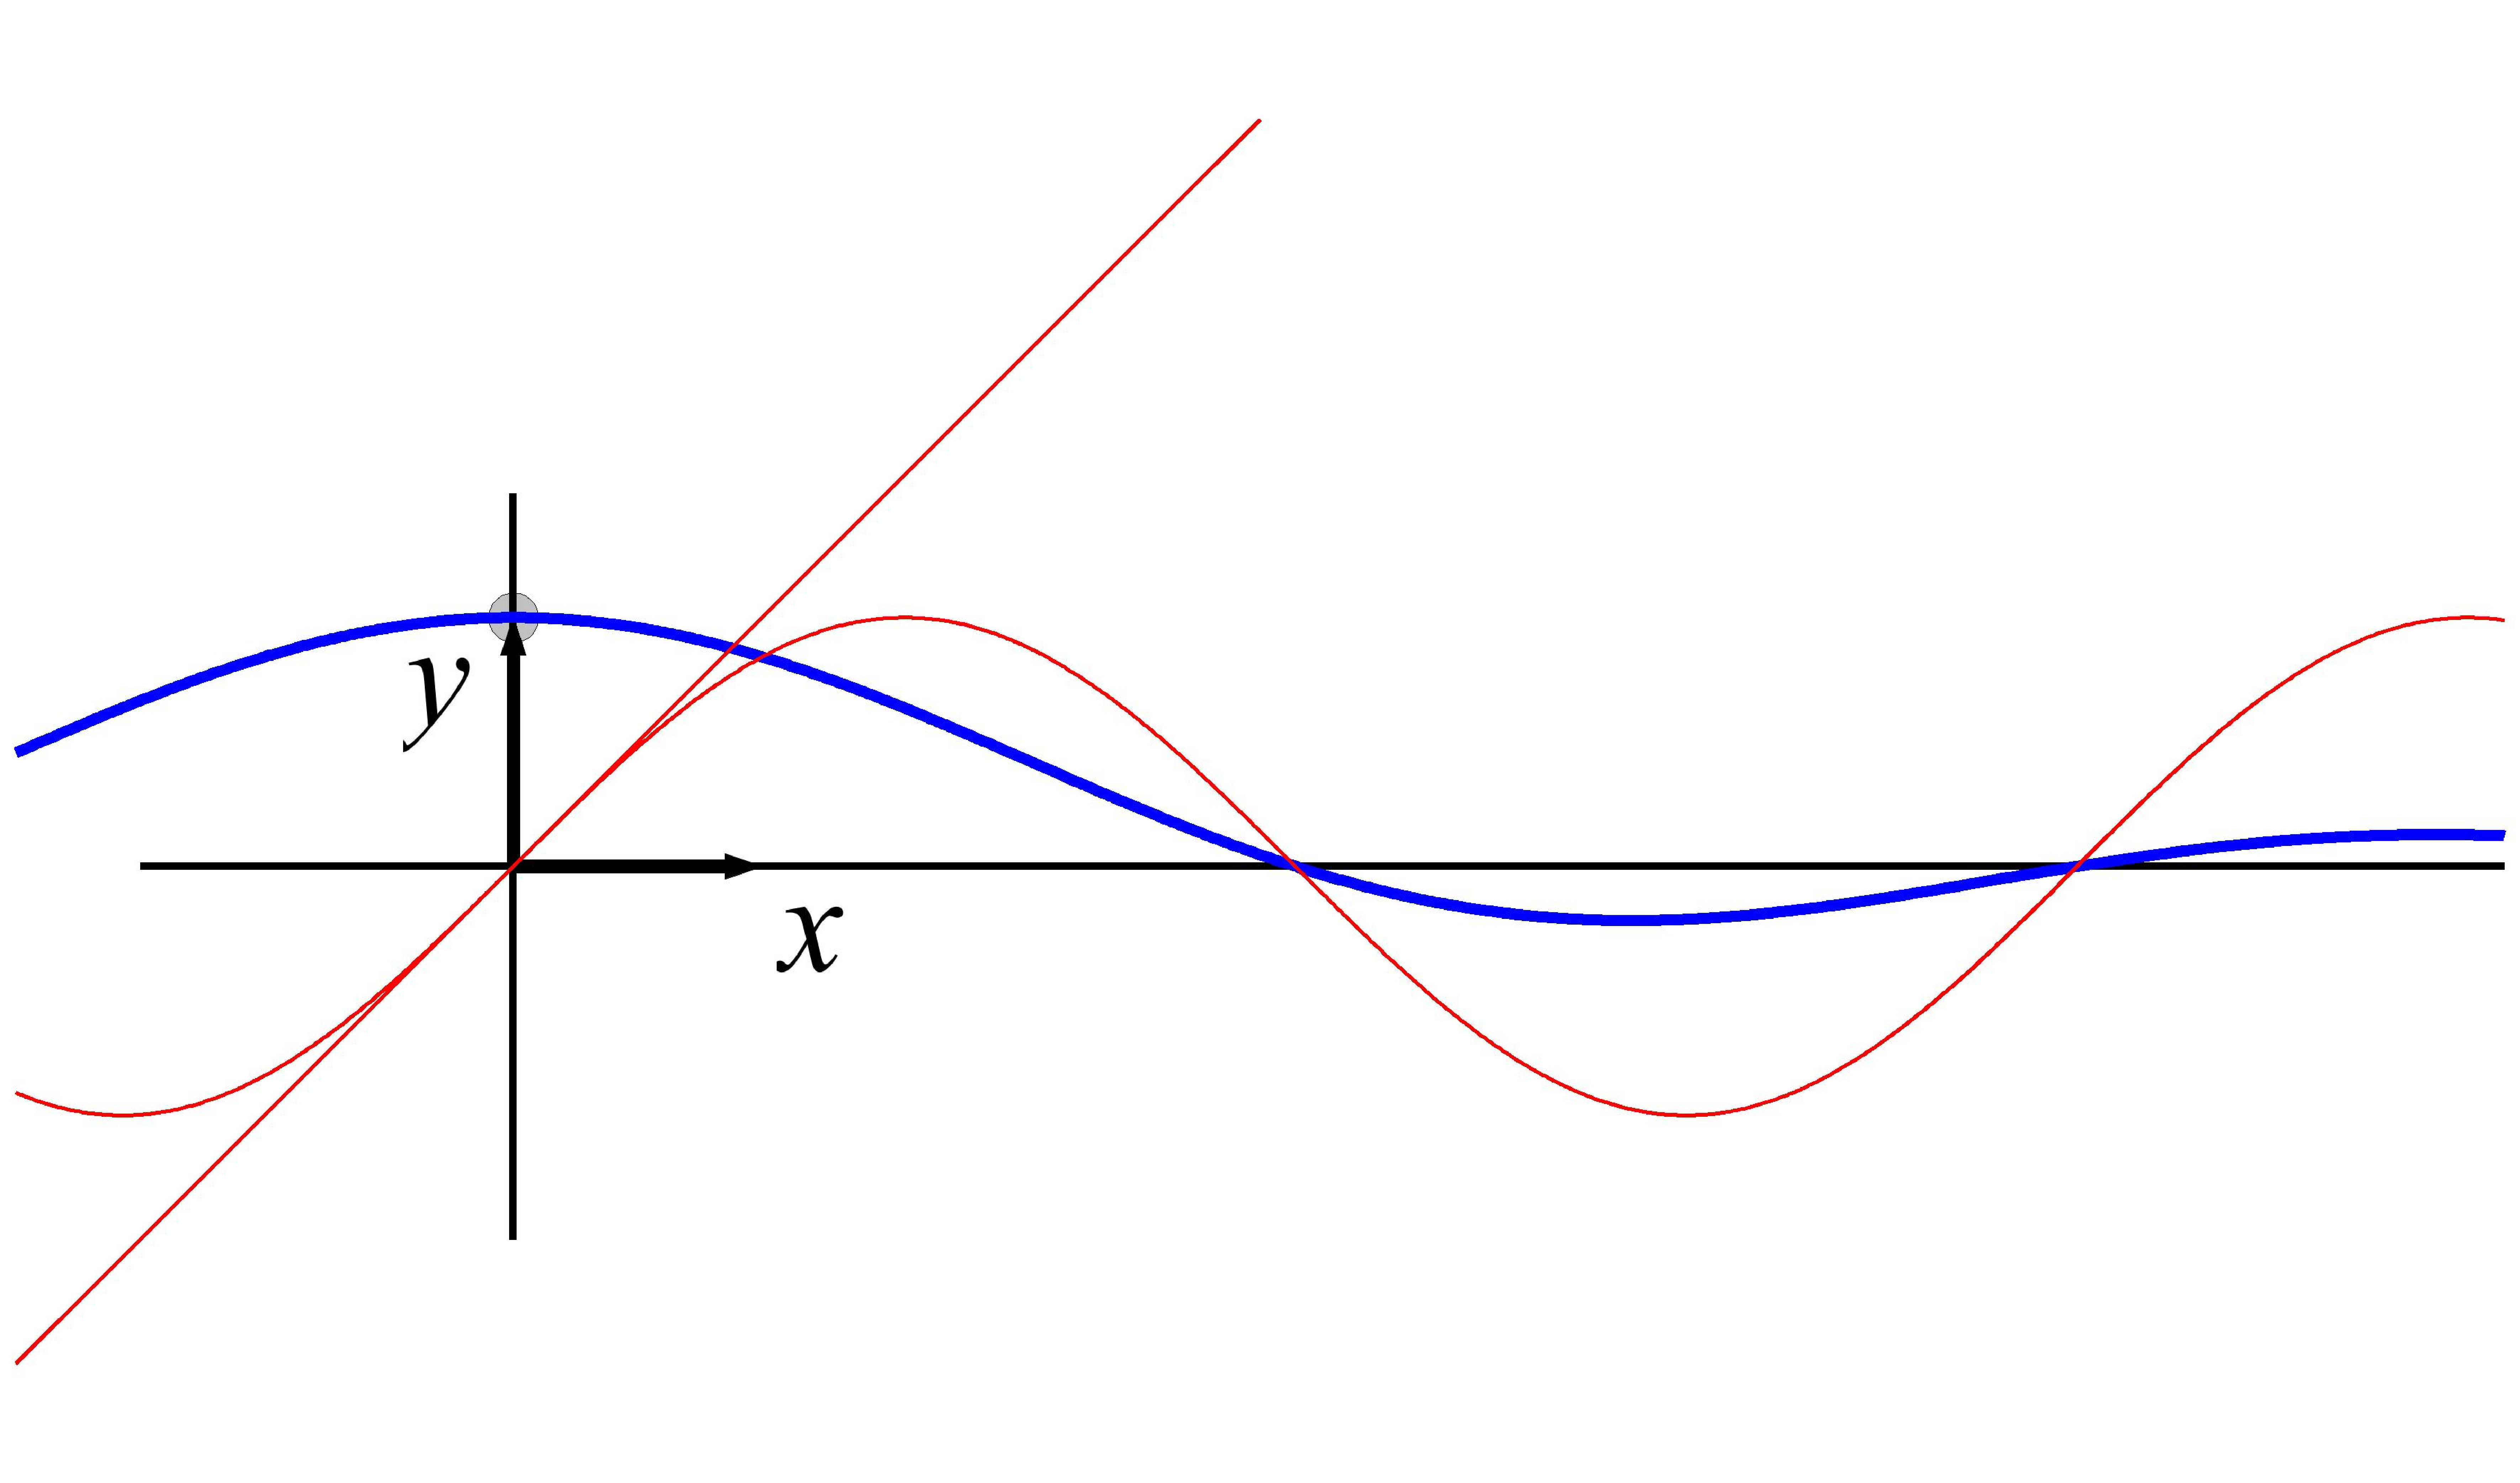
\includegraphics[height=75mm]{plotsinxdivx.pdf}}
\begin{center}
\caption{Funktionen $f(x)=\sin(x)/x$ (blå) sammen med tællerfunktionen $\sin(x)$ (rød) og nævnerfunktionen $x$ (også rød). Funktionen $f(x)$ er kontinuert i $x=0$ netop når den tildeles værdien $1$ der.} \label{figsinxdivx}
\end{center}
\end{figure}


\begin{example}[Grænseværdi for funktionsbrøk]
\begin{equation}
\begin{aligned}
\frac{2\cos(x) - 2 + x^{2}}{x\cdot\sin(x) - x^{2}} &= \frac{2\cdot(1 - \frac{1}{2!}\cdot x^{2} + \frac{1}{4!}\cdot x^{4} + x^{4}\cdot\varepsilon_{1}(x)) - 2 + x^{2}}{x\cdot(x-\frac{1}{3!}\cdot x^{3} + \frac{1}{5!}\cdot x^{5} + x^{5}\cdot \varepsilon_{2}(x) ) - x^{2}} \\
&=\frac{2 -  x^{2} + \frac{1}{12}\cdot x^{4} + 2\cdot x^{4}\cdot\varepsilon_{1}(x) - 2 + x^{2}}{x^{2} -\frac{1}{3!}\cdot x^{4} + \frac{1}{5!}\cdot x^{6} + x^{6}\cdot \varepsilon_{2}(x)  - x^{2}} \\
&=\frac{\frac{1}{12}\cdot x^{4} + 2\cdot x^{4}\cdot\varepsilon_{1}(x)}{-\frac{1}{3!}\cdot x^{4} + \frac{1}{5!}\cdot x^{6} + x^{6}\cdot \varepsilon_{2}(x) }\\
&=\frac{\frac{1}{12} + 2\cdot \varepsilon_{1}(x)}{-\frac{1}{6} + \frac{1}{5!}\cdot x^{2} + x^{2}\cdot \varepsilon_{2}(x) } \\
& \to -\frac{1}{2} \quad \textrm{for} \quad x \to 0 \quad ,
\end{aligned}
\end{equation}
idet tælleren går imod $\frac{1}{12}$ for $ x \to 0 $ og nævneren går imod $-\frac{1}{6}$ for $ x \to 0 $.
\end{example}

\section{Vurdering af restfunktionerne} \label{secVurderingRest}

Hvor stor er den fejl man begår ved at benytte det approksimerende polynomium (som er let at regne med) i stedet for funktionen selv (som kan være kompliceret at beregne) i et givet (typisk lille) interval omkring udviklingspunktet? Det kan restfunktionen selvfølgelig give et svar på. Vi giver her et par eksempler der viser, hvordan restfunktions\-udtrykket kan benyttes til sådanne fejl-vurderinger for givne funktioner.


\begin{figure}[ht]
\centerline{ 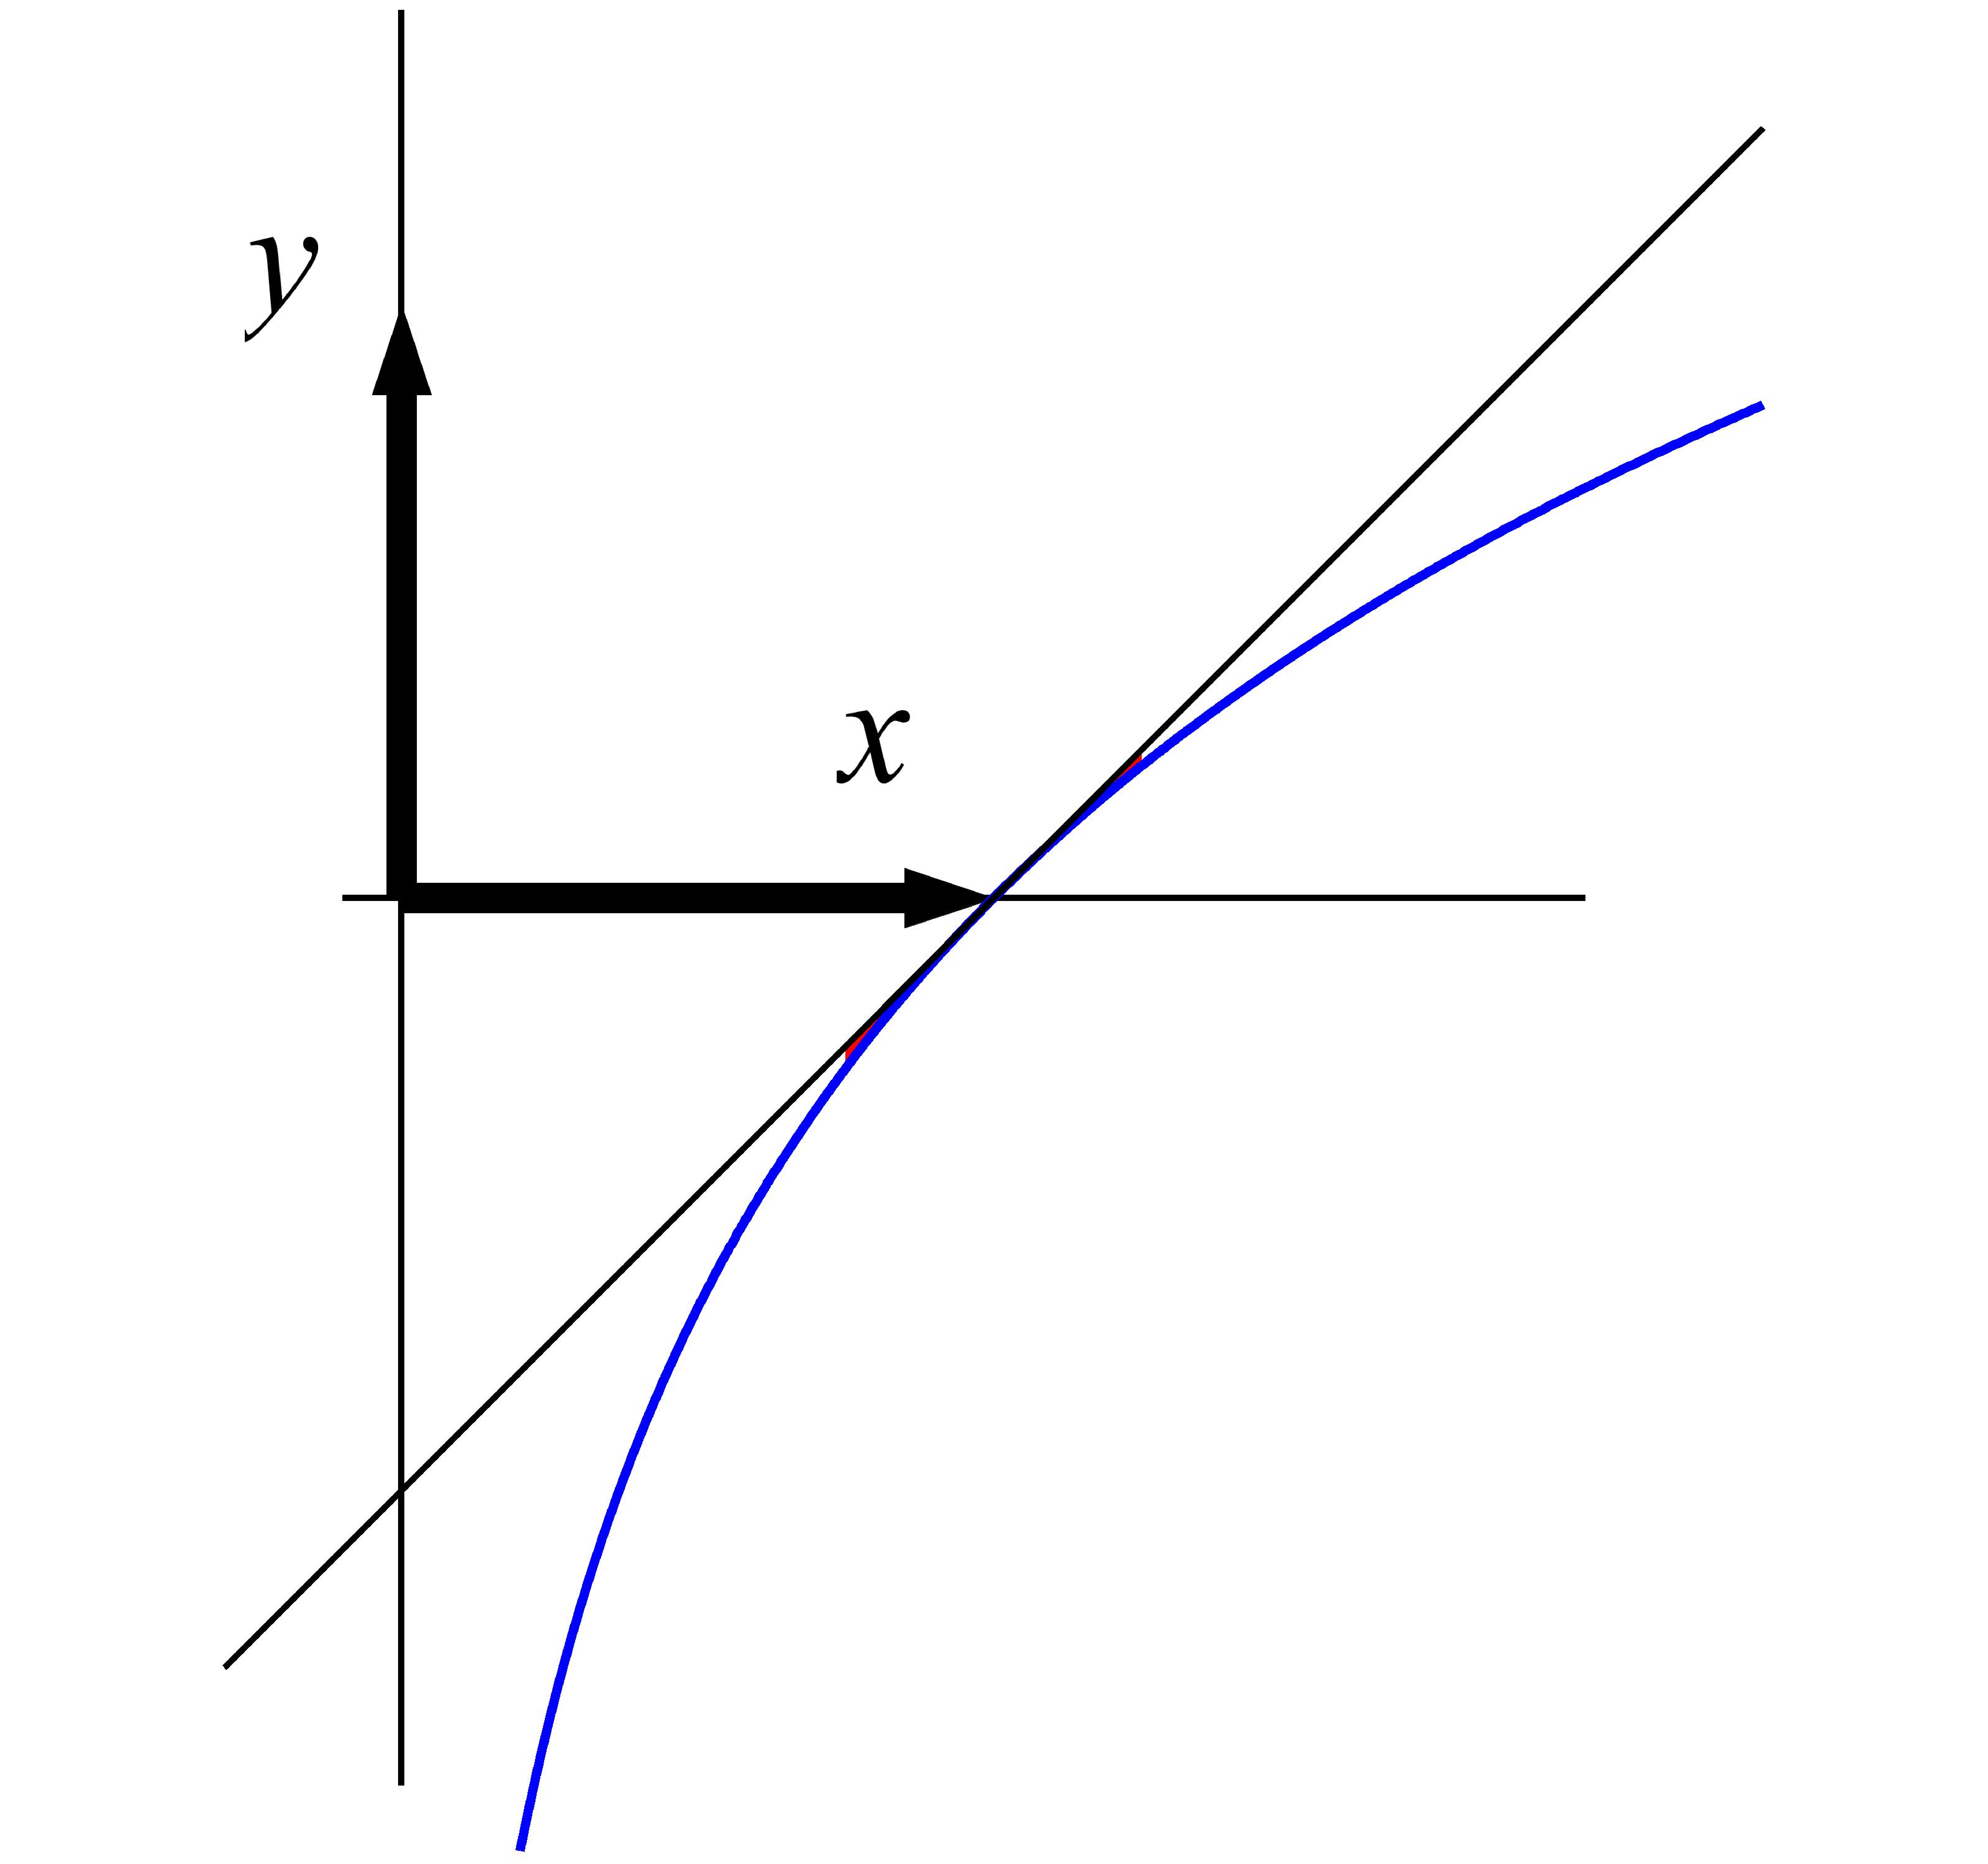
\includegraphics[height=55mm]{plotLn.pdf} 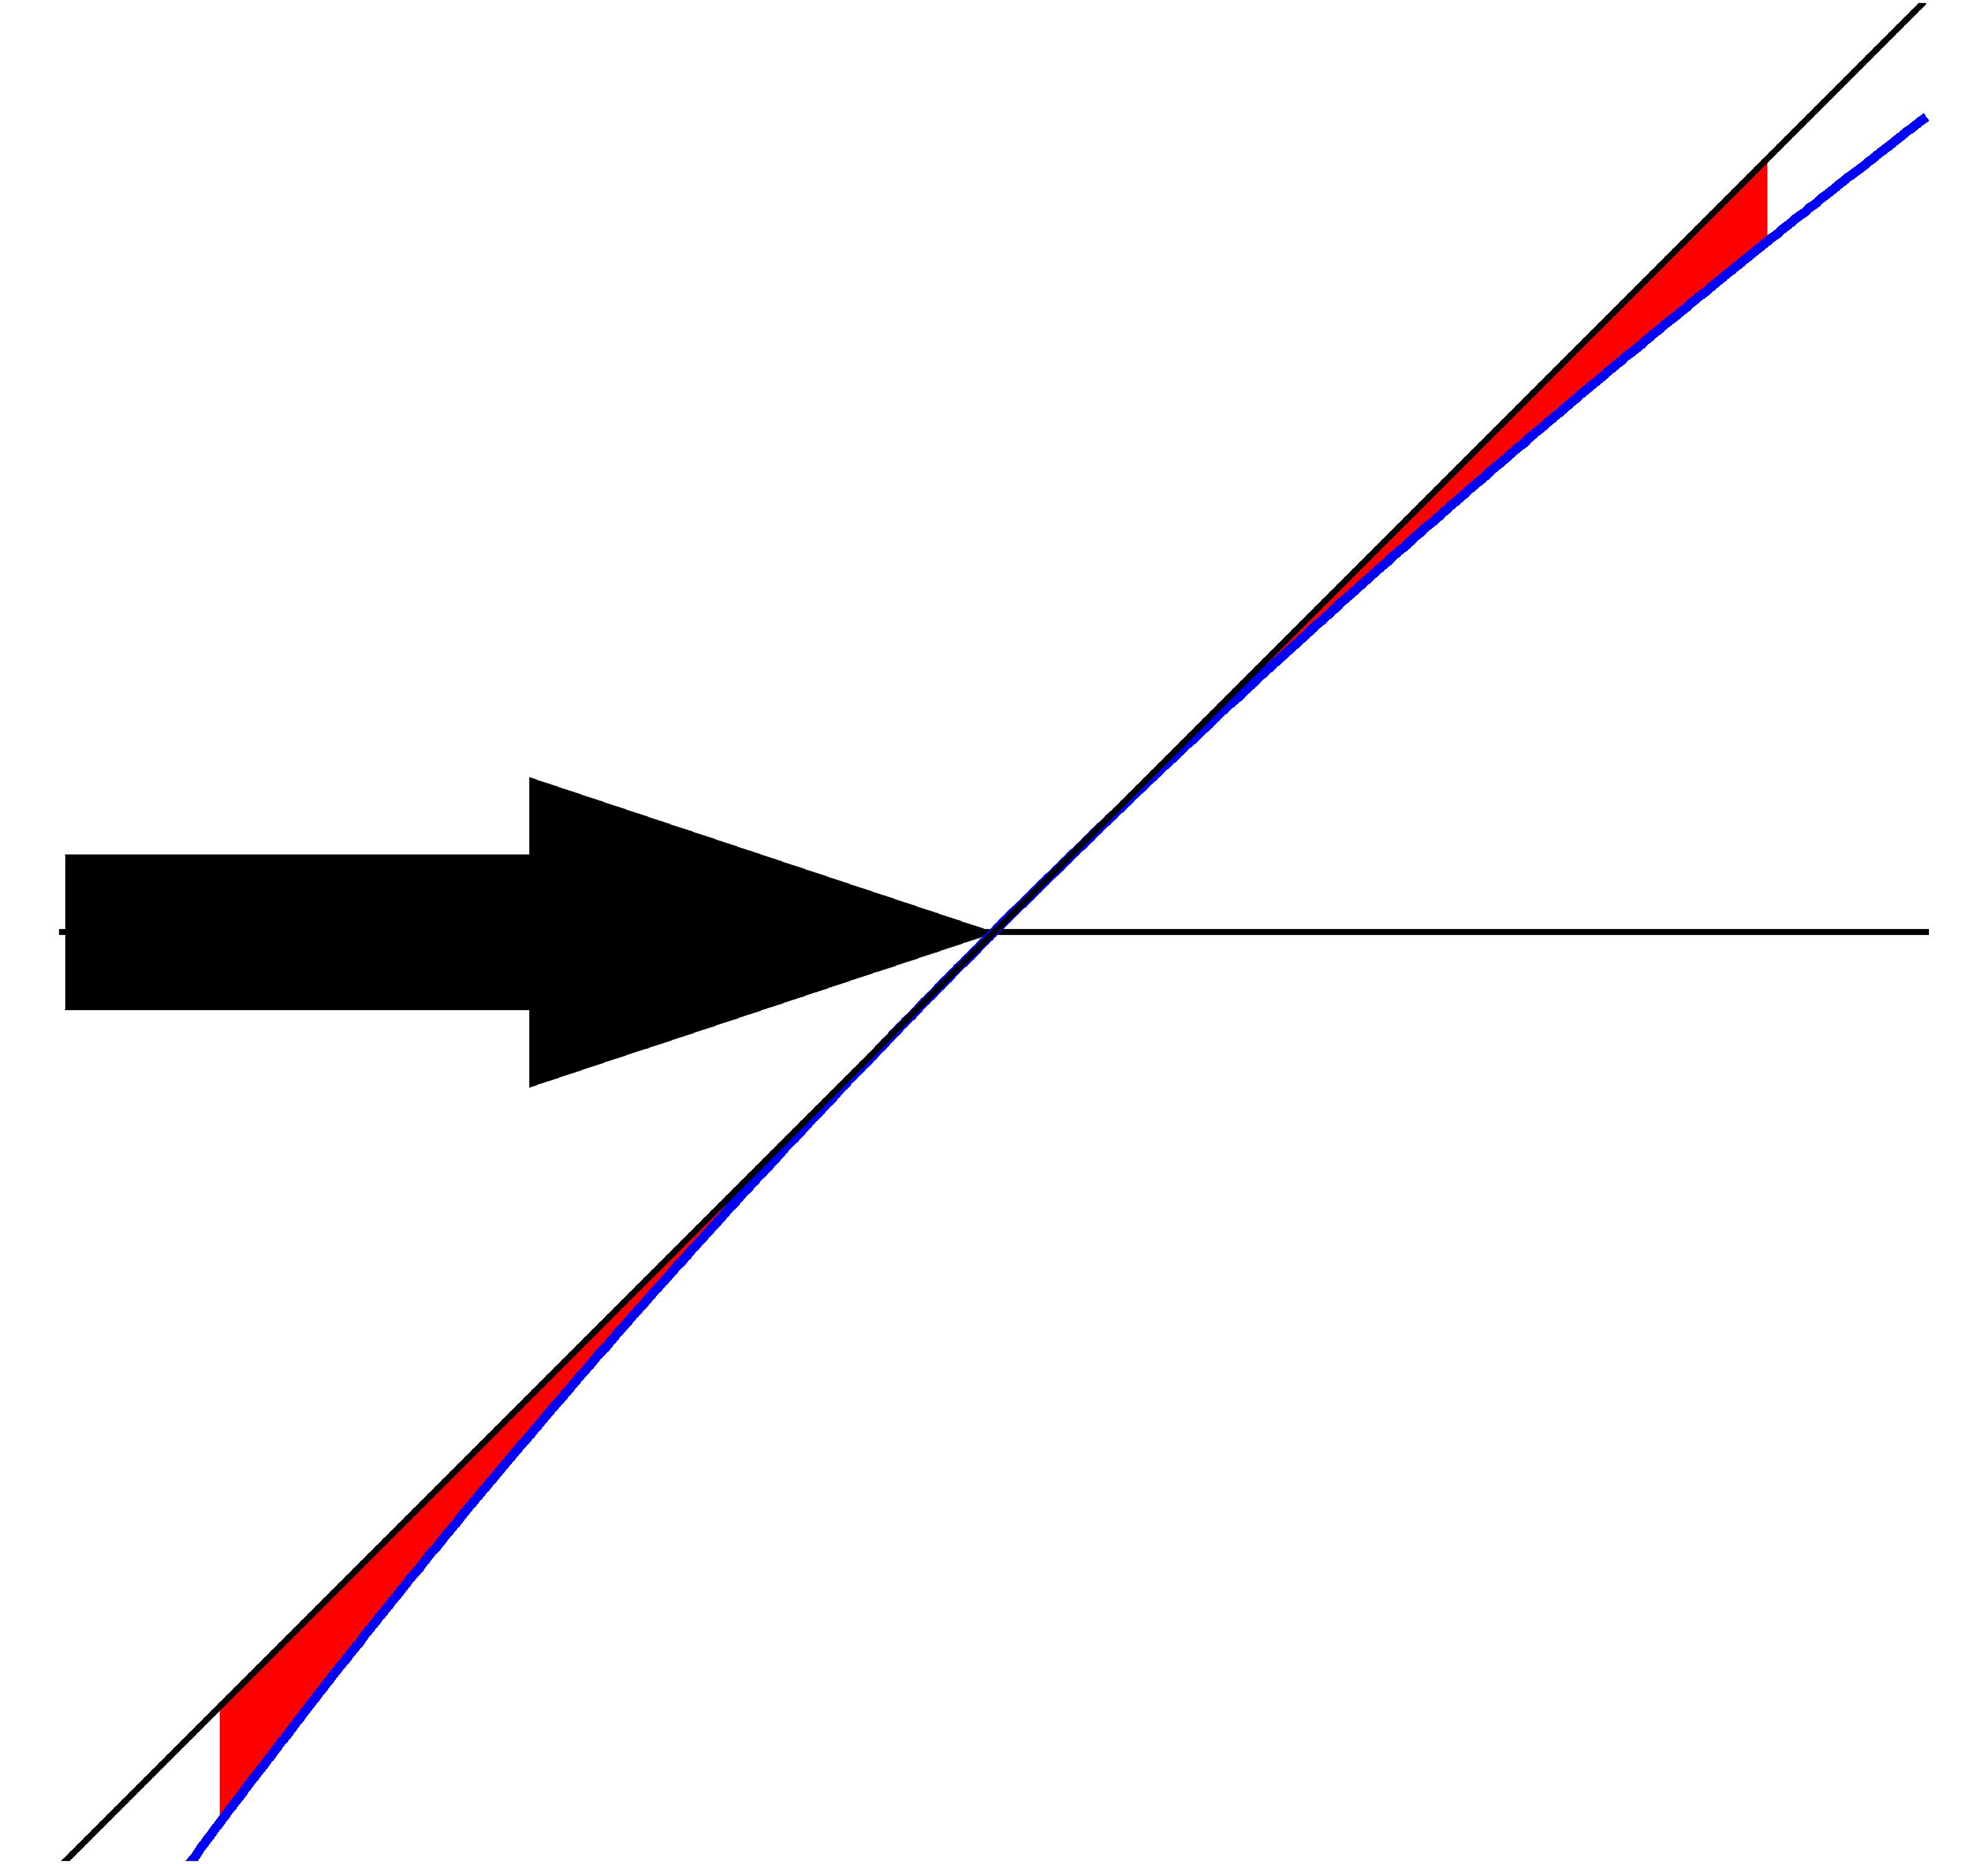
\includegraphics[height=55mm]{plotLnZoom.pdf}}
\begin{center}
\caption{Funktionen $f(x) = \ln(x)$ fra eksempel \ref{exampRestVurdering0} (blå), det approksimerende første-gradspolynomium (sort) med udviklingspunkt $x_{0}=1$ og den tilhørende restfunktion (rød) illustreret som forskellen mellem $f(x)$ og det approksimerende polynomium i intervallet $\left[\frac{3}{4}, \frac{5}{4}\right]$. Til højre er zoomet ind på figuren omkring punktet $(1,0)$.} \label{figLn}
\end{center}
\end{figure}

\begin{example}[Approksimation af elementær funktion] \label{exampRestVurdering0}
Logaritmefunktionen $\ln(x)$ er defineret for positive værdier af $x$. Vi approksimerer med det approksimerende førstegrads-polynomium med udviklingspunkt i $x_{0}=1$ og vil vurdere restleddet i et passende lille interval omkring $x_{0}=1$, dvs. udgangspunktet er følgende:
\begin{equation}
f(x) = \ln(x) \quad , \quad x_{0}=1 \quad ,\quad  n = 1 \quad , \quad x \in \left[\frac{3}{4}, \frac{5}{4} \right] \quad .
\end{equation}
Ifølge Taylor's formel med restfunktion har vi - idet vi udvikler i udviklingspunktet $x_{0}=1$ hvor $f(1) = 0$ og $f'(1) = 1$ og bruger
$f''(x) = -1/x^{2}$ for alle $x$ i definitionsmængden:
\begin{equation}
f(x) = \ln(x) = \ln(1) + \frac{f'(1)}{1!}(x-1) + \frac{f''(\xi)}{2!}\cdot(x-1)^{2} = x-1 - \frac{1}{2\cdot \xi^{2}}\cdot (x-1)^{2}
\end{equation}
for en værdi af $\xi$ imellem $x$ og $1$.
Vi har altså hermed fundet:
\begin{equation}
P_{1,x_{0}=1}(x) = x-1 \quad , \quad \textrm{og} \quad R_{1, x_{0}=1}(x) = - \frac{1}{2\cdot \xi^{2}}\cdot (x-1)^{2} \quad.
\end{equation}
Den {\emph{numeriske værdi af restfunktionen}} i det givne interval kan nu vurderes for alle $x$ i det givne interval - også selvom vi ikke ved ret meget om hvor $\xi$ ligger i intervallet udover at $\xi$ ligger imellem $x$ og $1$:\\

Vi har
\begin{equation}
|R_{1, x_{0}=1}(x)| = |- \frac{1}{2\cdot \xi^{2}}\cdot (x-1)^{2}| \leq |\frac{1}{2\cdot \xi^{2}}\cdot \left(\frac{1}{4}\right)^{2}| \quad ,
\end{equation}
idet minus-tegnet kan fjernes fordi vi kun ser på den numeriske værdi og idet $(x-1)^{2}$ jo klart er størst (med værdien $(1/4)^{2}$) for $x=3/4$ og for $x=5/4$ i intervallet.
Derudover er $\xi$ {\emph{mindst}} og dermed $(1/\xi)^{2}$ {\emph{størst}} i intervallet for $\xi = 3/4$. (Bemærk at vi ikke bruger her, at $\xi$ ligger imellem $x$ og $1$ - vi bruger kun, at $\xi$ ligger i intervallet!)
Det vil sige, at
\begin{equation}
|R_{1, x_{0}=1}(x)| \leq |\frac{1}{32\cdot\xi^{2}}| \leq |\frac{1}{32\cdot\left(\frac{3}{4}\right)^{2}}| = \frac{1}{18} \quad,
\end{equation}
således at vi dermed har vist, at
\begin{equation}
|\ln(x) - (x-1)| \leq \frac{1}{18} \quad \textrm{for alle} \quad x \in \left[\frac{3}{4}, \frac{5}{4} \right] \quad .
\end{equation}
\end{example}


\begin{think}
Man kan med nogen ret spekulere over, hvorfor restfunktions-vurderingen  af en så simpel funktion som $f(x) = \ln(x)$ i eksempel \ref{exampRestVurdering0} skal være så bøvlet, når det er tydeligt for enhver (!), at den røde restfunktion i det tilfælde antager sin største numeriske (absolut-)værdi i et af endepunkterne i det aktuelle interval, se figur \ref{figLn} -- en påstand som vi endda kan vise med en helt almindelig funktionsundersøgelse. \\

Ved at differentiere restfunktionen får vi jo:
\begin{equation}
R'_{1, x_{0}=1}(x) = \frac{d}{dx}\left(\ln(x) - (x-1) \right) = \frac{1}{x} - 1 \quad,
\end{equation}
som netop er mindre end $0$ for $x >1$ (sådan at $R_{1, x_{0}=1}(x) $ til højre for $x=1$ er negativ og aftagende fra værdien $0$ i $x=1$) og større end $0$ for $x <1$
 (sådan at $R_{1, x_{0}=1}(x) $ til venstre for $x=1$ er negativ og voksende op mod værdien $0$ i $x=1$). Men problemet er, at vi {\emph{i princippet ikke ved}}  hvad værdien af  $\ln(x)$ faktisk er -- hverken i $x=3/4$ eller i $x=5/4$ medmindre vi bruger Maple eller et andet værktøj til hjælp. Restfunktions-vurderingen benytter {\emph{kun}} de definerende egen\-ska\-ber ved $f(x) = \ln(x)$, dvs. $f'(x) = 1/x$ og $f(1)=0$, og vurderingen giver værdierne (også i endepunkterne af intervallet) med en (numerisk) fejl på højst $1/18$ i dette tilfælde. \\

 {\emph{Hvis}} vi faktisk får serveret  den oplysning, at
 $\ln(3/4) = -0.2877$ og  $\ln(5/4) = 0.2223$ så har vi selvfølgelig dermed også en direkte vurdering af den største værdi af $|R_{1, x_{0}=1}(x)|$ i intervallet $\left[\frac{3}{4}, \frac{5}{4} \right]$:
 \begin{equation}
 \begin{aligned}
 |R_{1, x_{0}=1}(x)| &\leq \max\{|-0.2877 + 0.25| \, , \, |0.2223 - 0.25| \} \\
  &= 0.0377 < 1/18 = 0.0556 \quad.
 \end{aligned}
 \end{equation}
 Med den almindelige funktionsanalyse får vi altså en noget bedre vurdering af restfunktionen -- men kun fordi vi i forvejen kan vurdere værdien af funktionen  i endepunkterne.


\end{think}

\begin{figure}[ht]
\centerline{ 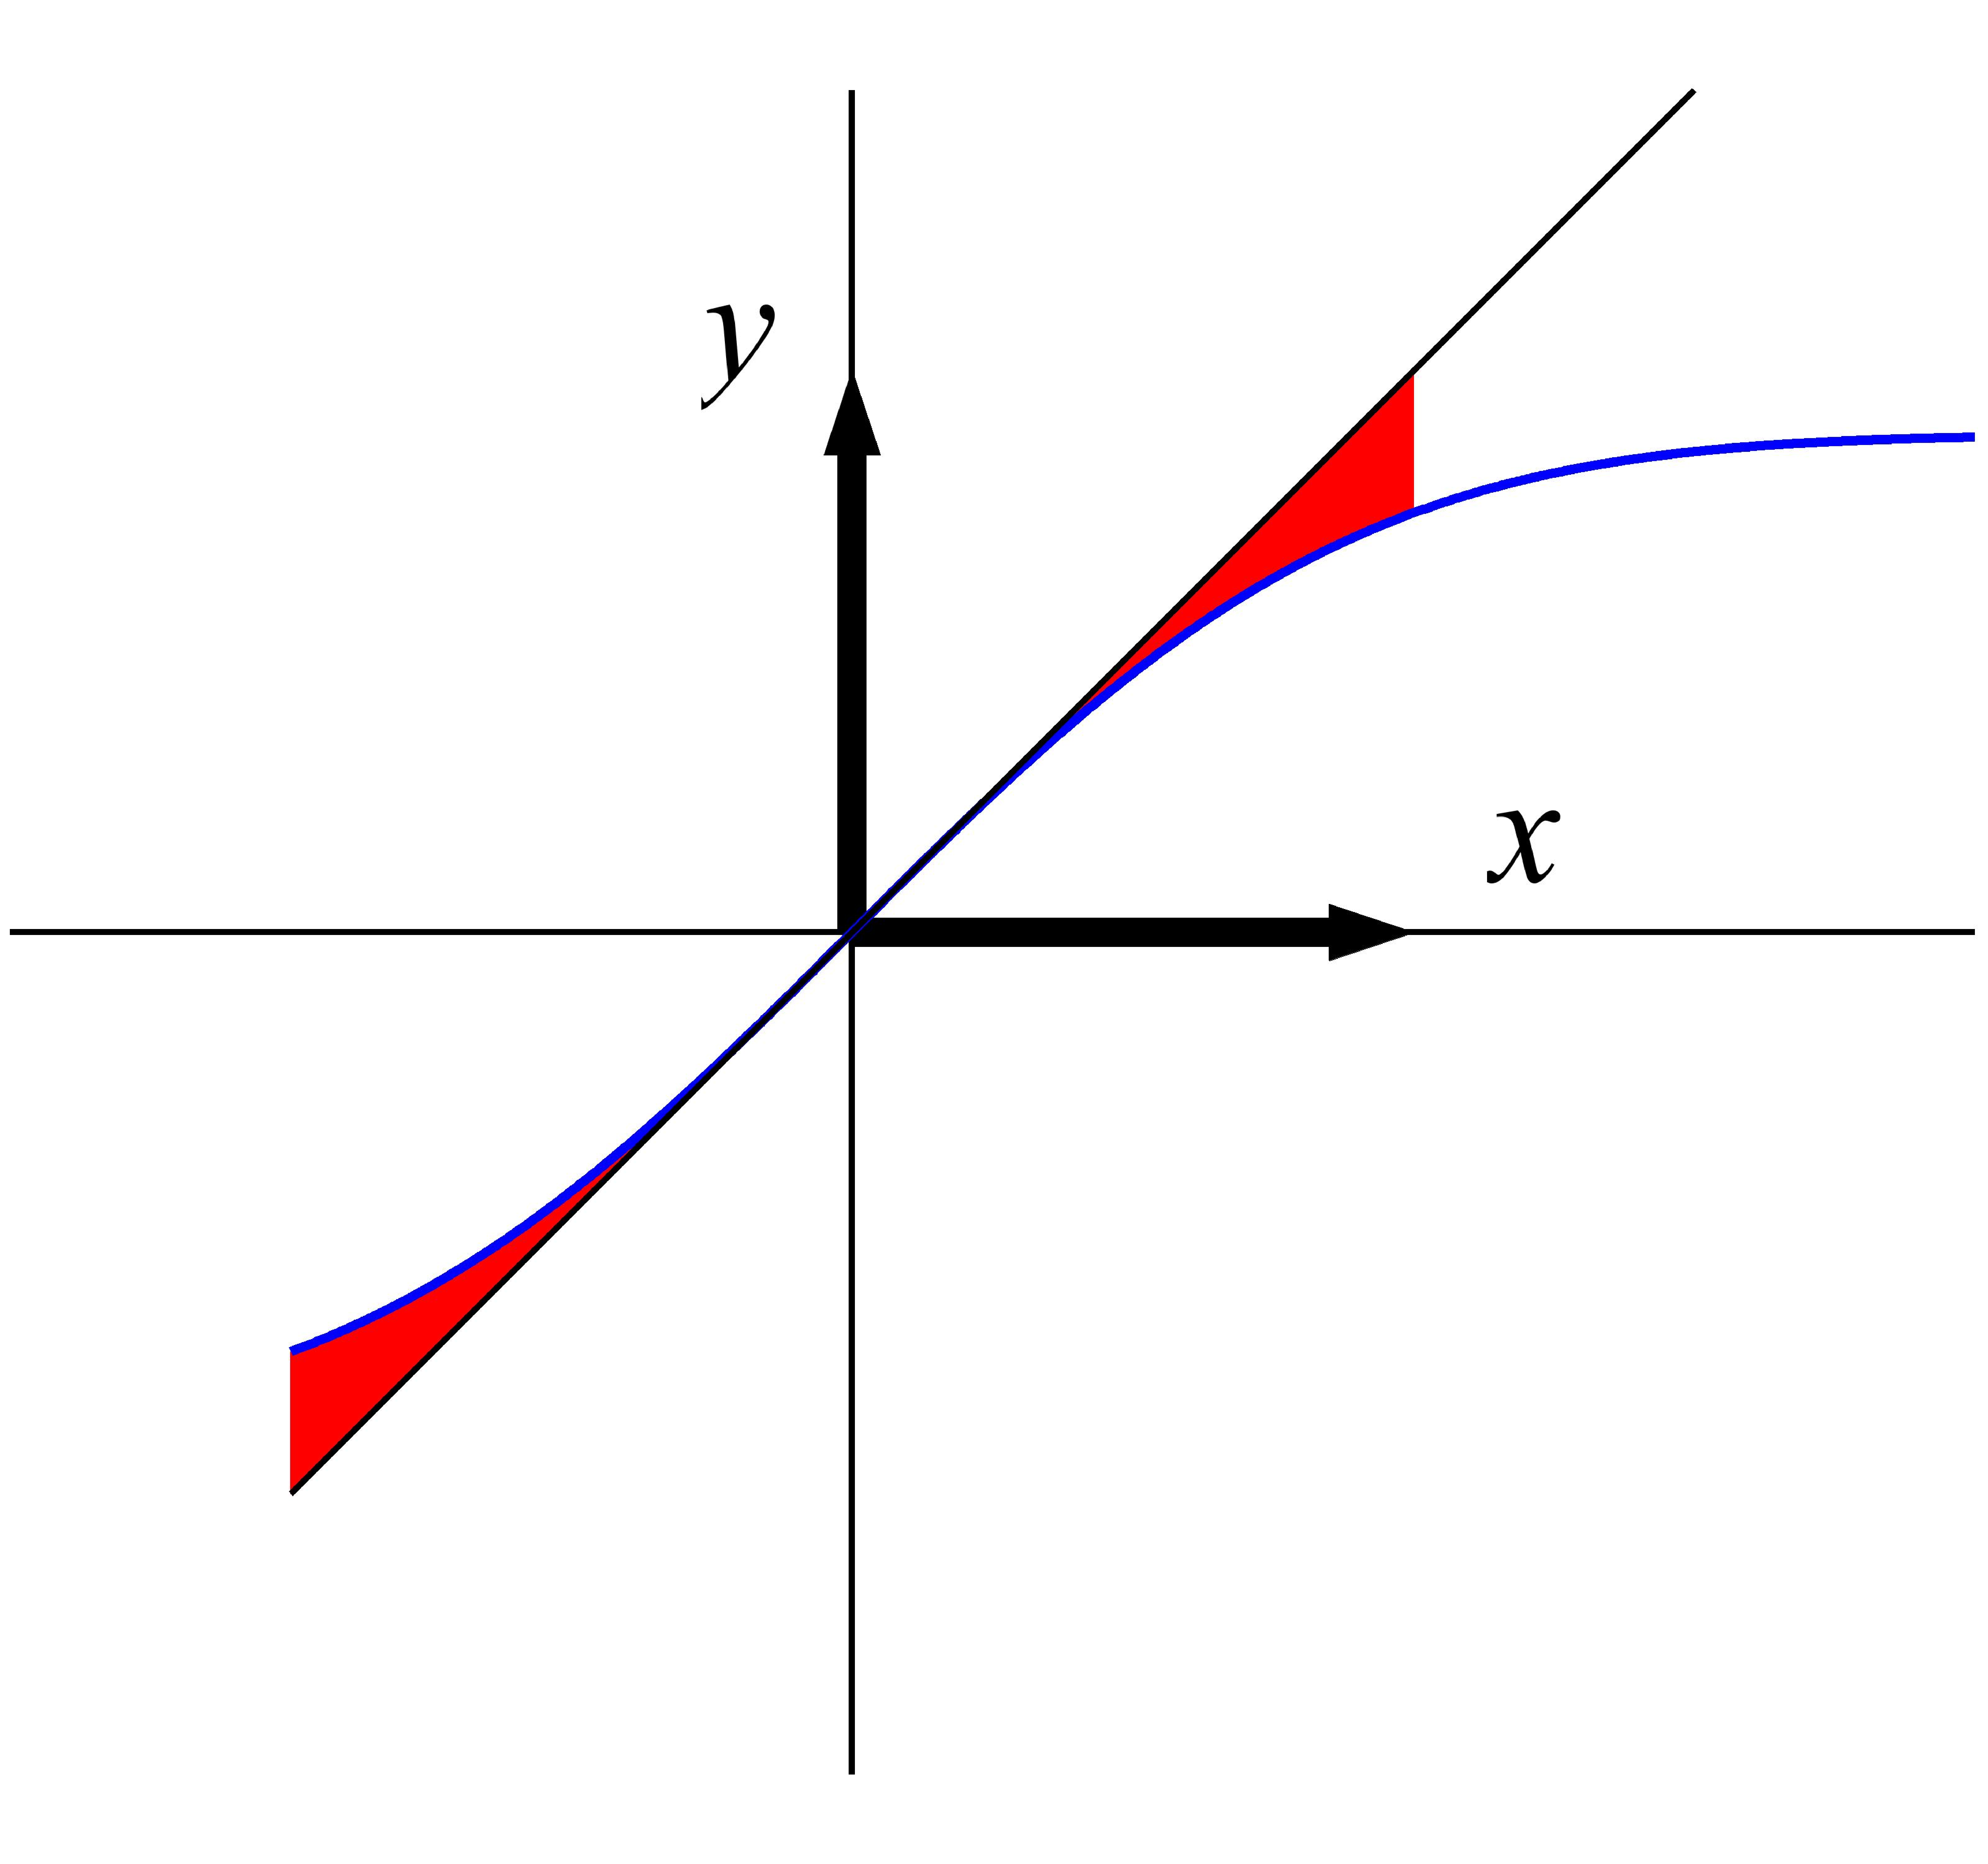
\includegraphics[height=55mm]{plotErf2.pdf} 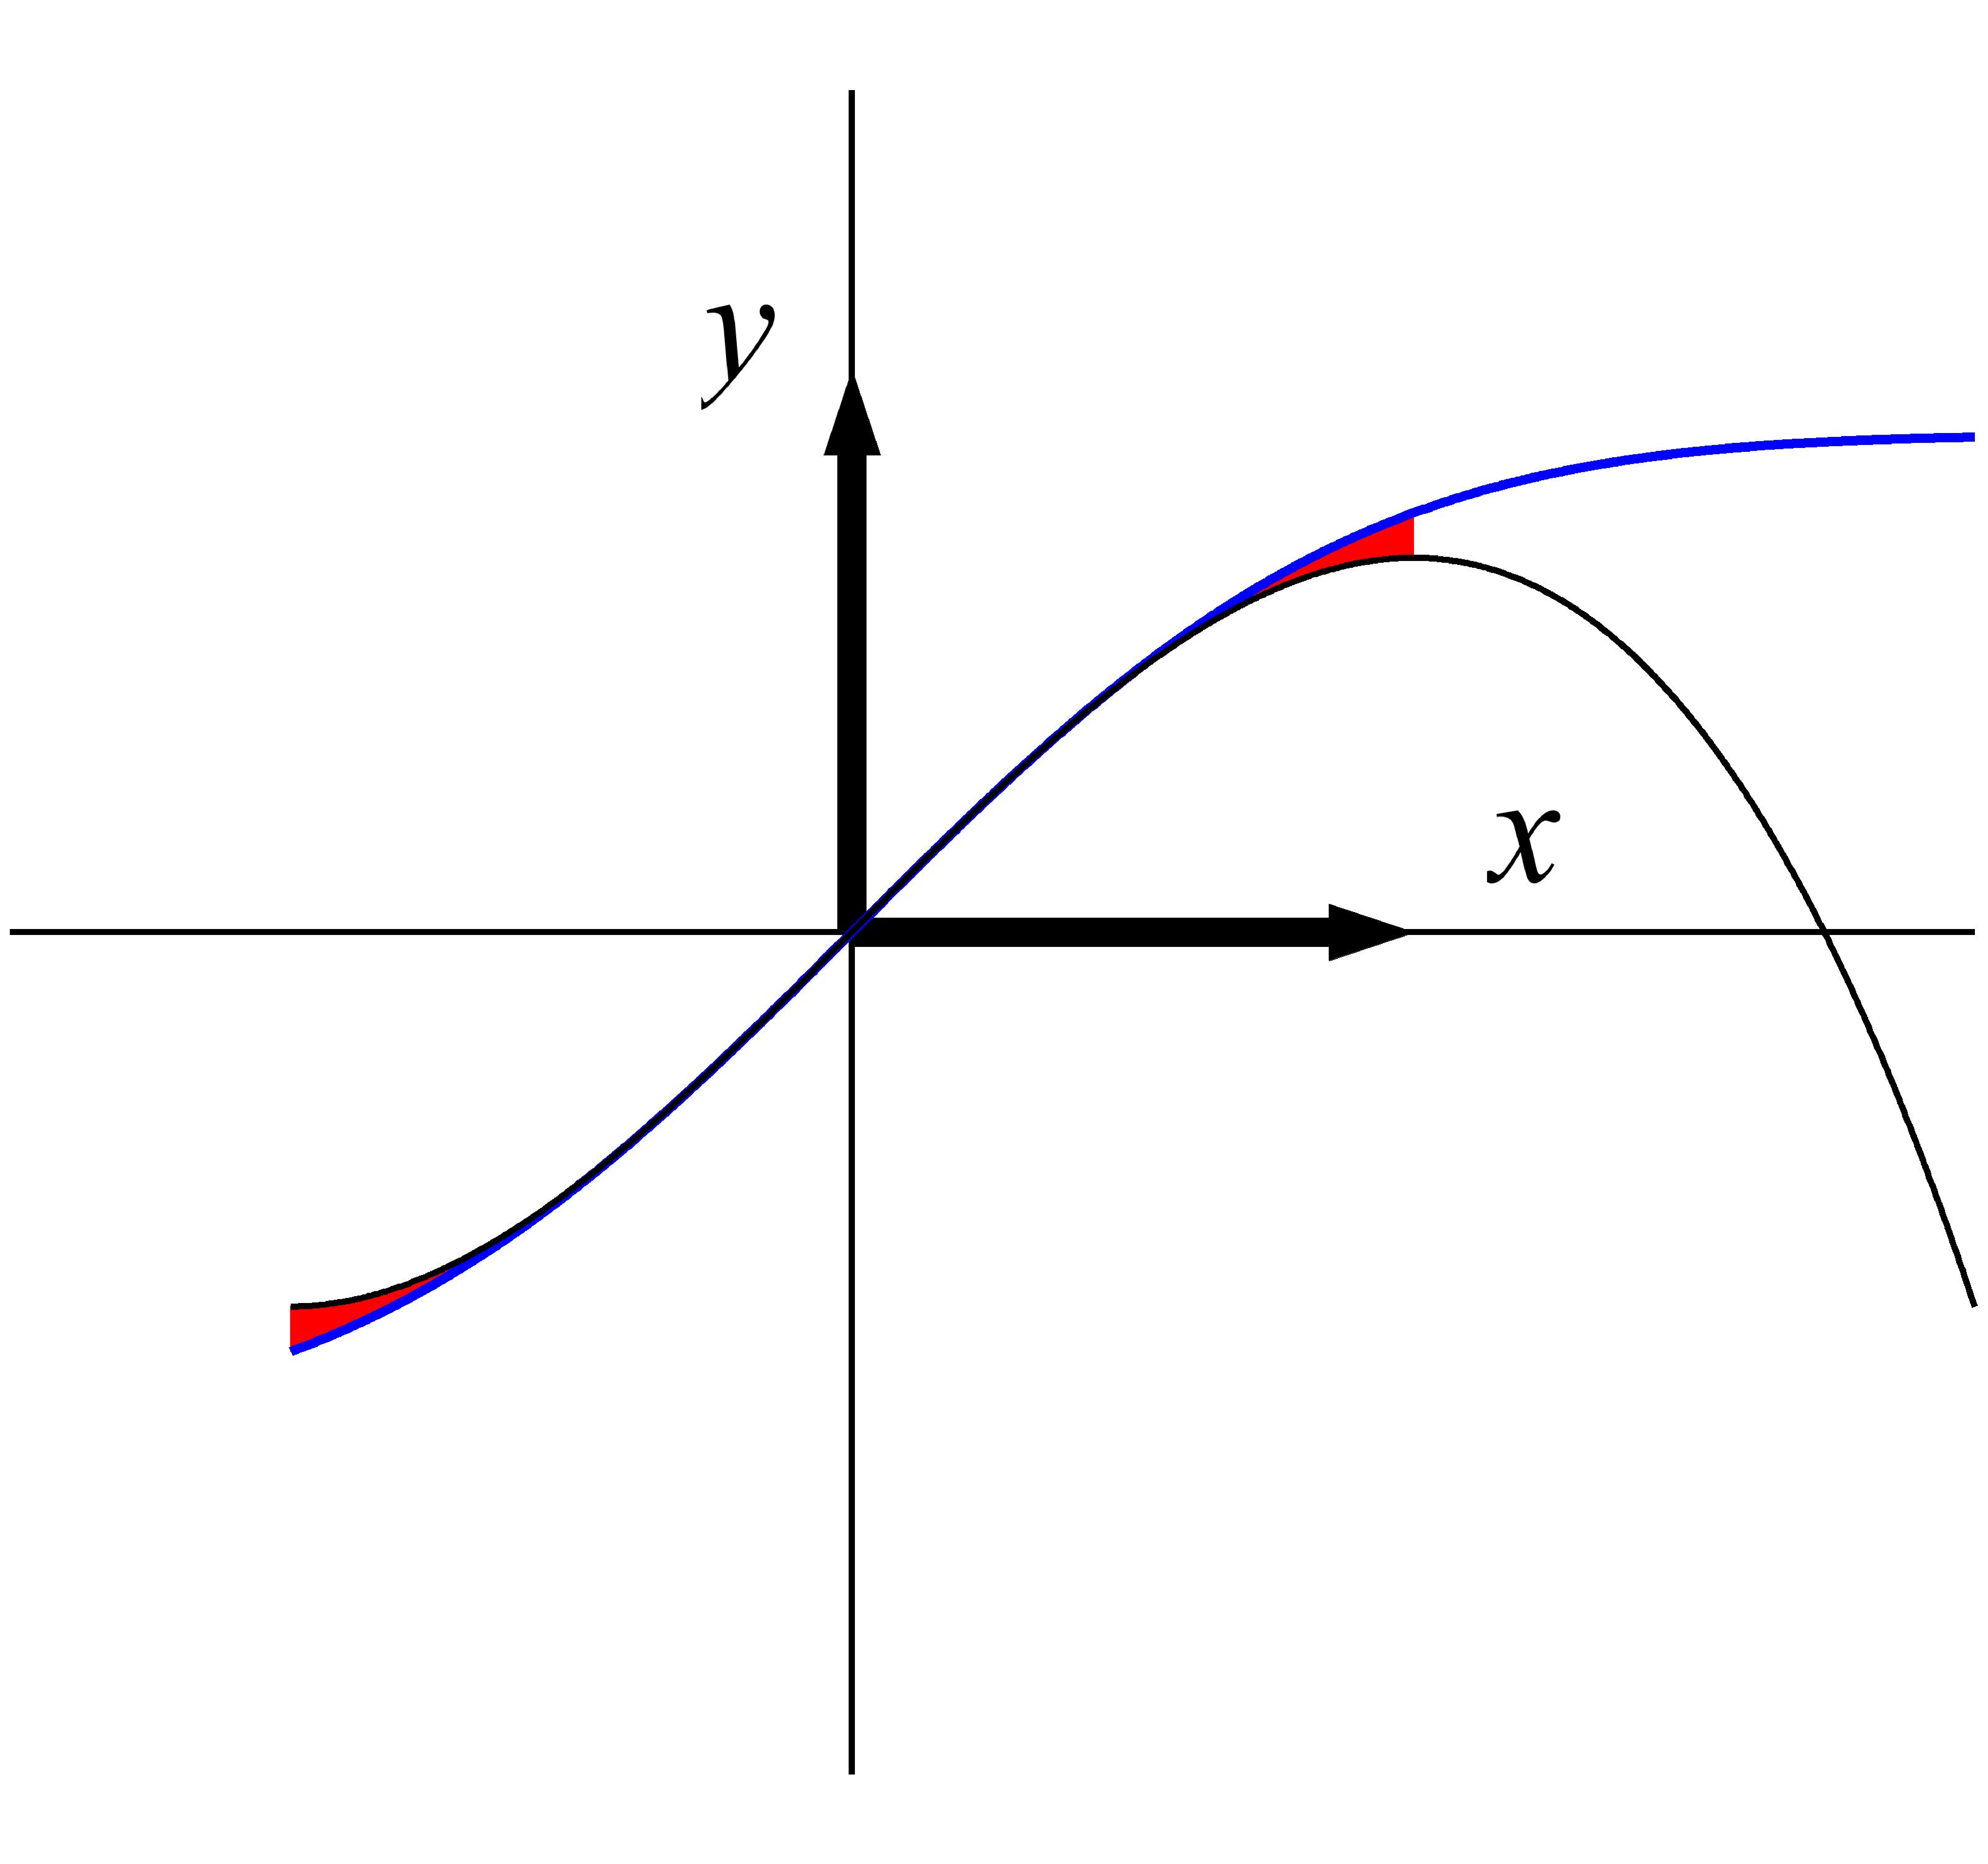
\includegraphics[height=55mm]{plotErf.pdf}}
\begin{center}
\caption{Funktionen $f(x)$ fra eksempel \ref{exampRestVurdering1} (blå), de approksimerende første- og tredjegrads-polynomier (sorte) med udviklingspunkt $x_{0}=0$ og de tilhørende restfunktioner (røde) i intervallet $[-1, 1]$.} \label{figErf}
\end{center}
\end{figure}



%%%%%%%%%%%%%%%%%%%%%%%%%%%%
%%%%%%%%%%%%%%%%%%%%%%%%%%%%
%%%%%%%%%%%%%%%%%%%%%%%%%%%%
%%%%%%%%%%%%%%%%%%%%%%%%%%%%



\begin{exercise}[Approksimation af en ikke-elementær funktion] \label{exampRestVurdering1}
Givet funktionen fra eksempel \ref{exampElemInt}:
\begin{equation}
f(x) = \int_{0}^{x}\,\e^{-t^{2}}\,dt
\end{equation}
Der ønskes en vurdering af størrelsen af forskellen mellem $f(x)$ og funktionens approksimerende førstegradspolynomium $P_{1, x_{0}=0}(x)$ med udviklingspunkt i $x_{0}=0$. Opgaven går altså ud på at bestemme den største absolut-værdi som restfunktionen $|R_{1, x_{0}=0}(x)|$ antager i intervallet $[-1, 1]$.\\
Vink: Benyt de tidligere fundne højere afledede af $f(x)$ evalueret i $x_{0}=0$, jvf. eksempel \ref{exampElemInt}: $f(0)=0$, $f'(0) = 1$, $f''(x)= -2\cdot x \cdot \e^{-x^{2}}$. Se figur \ref{figErf}.
\end{exercise}


\begin{figure}[ht]
\centerline{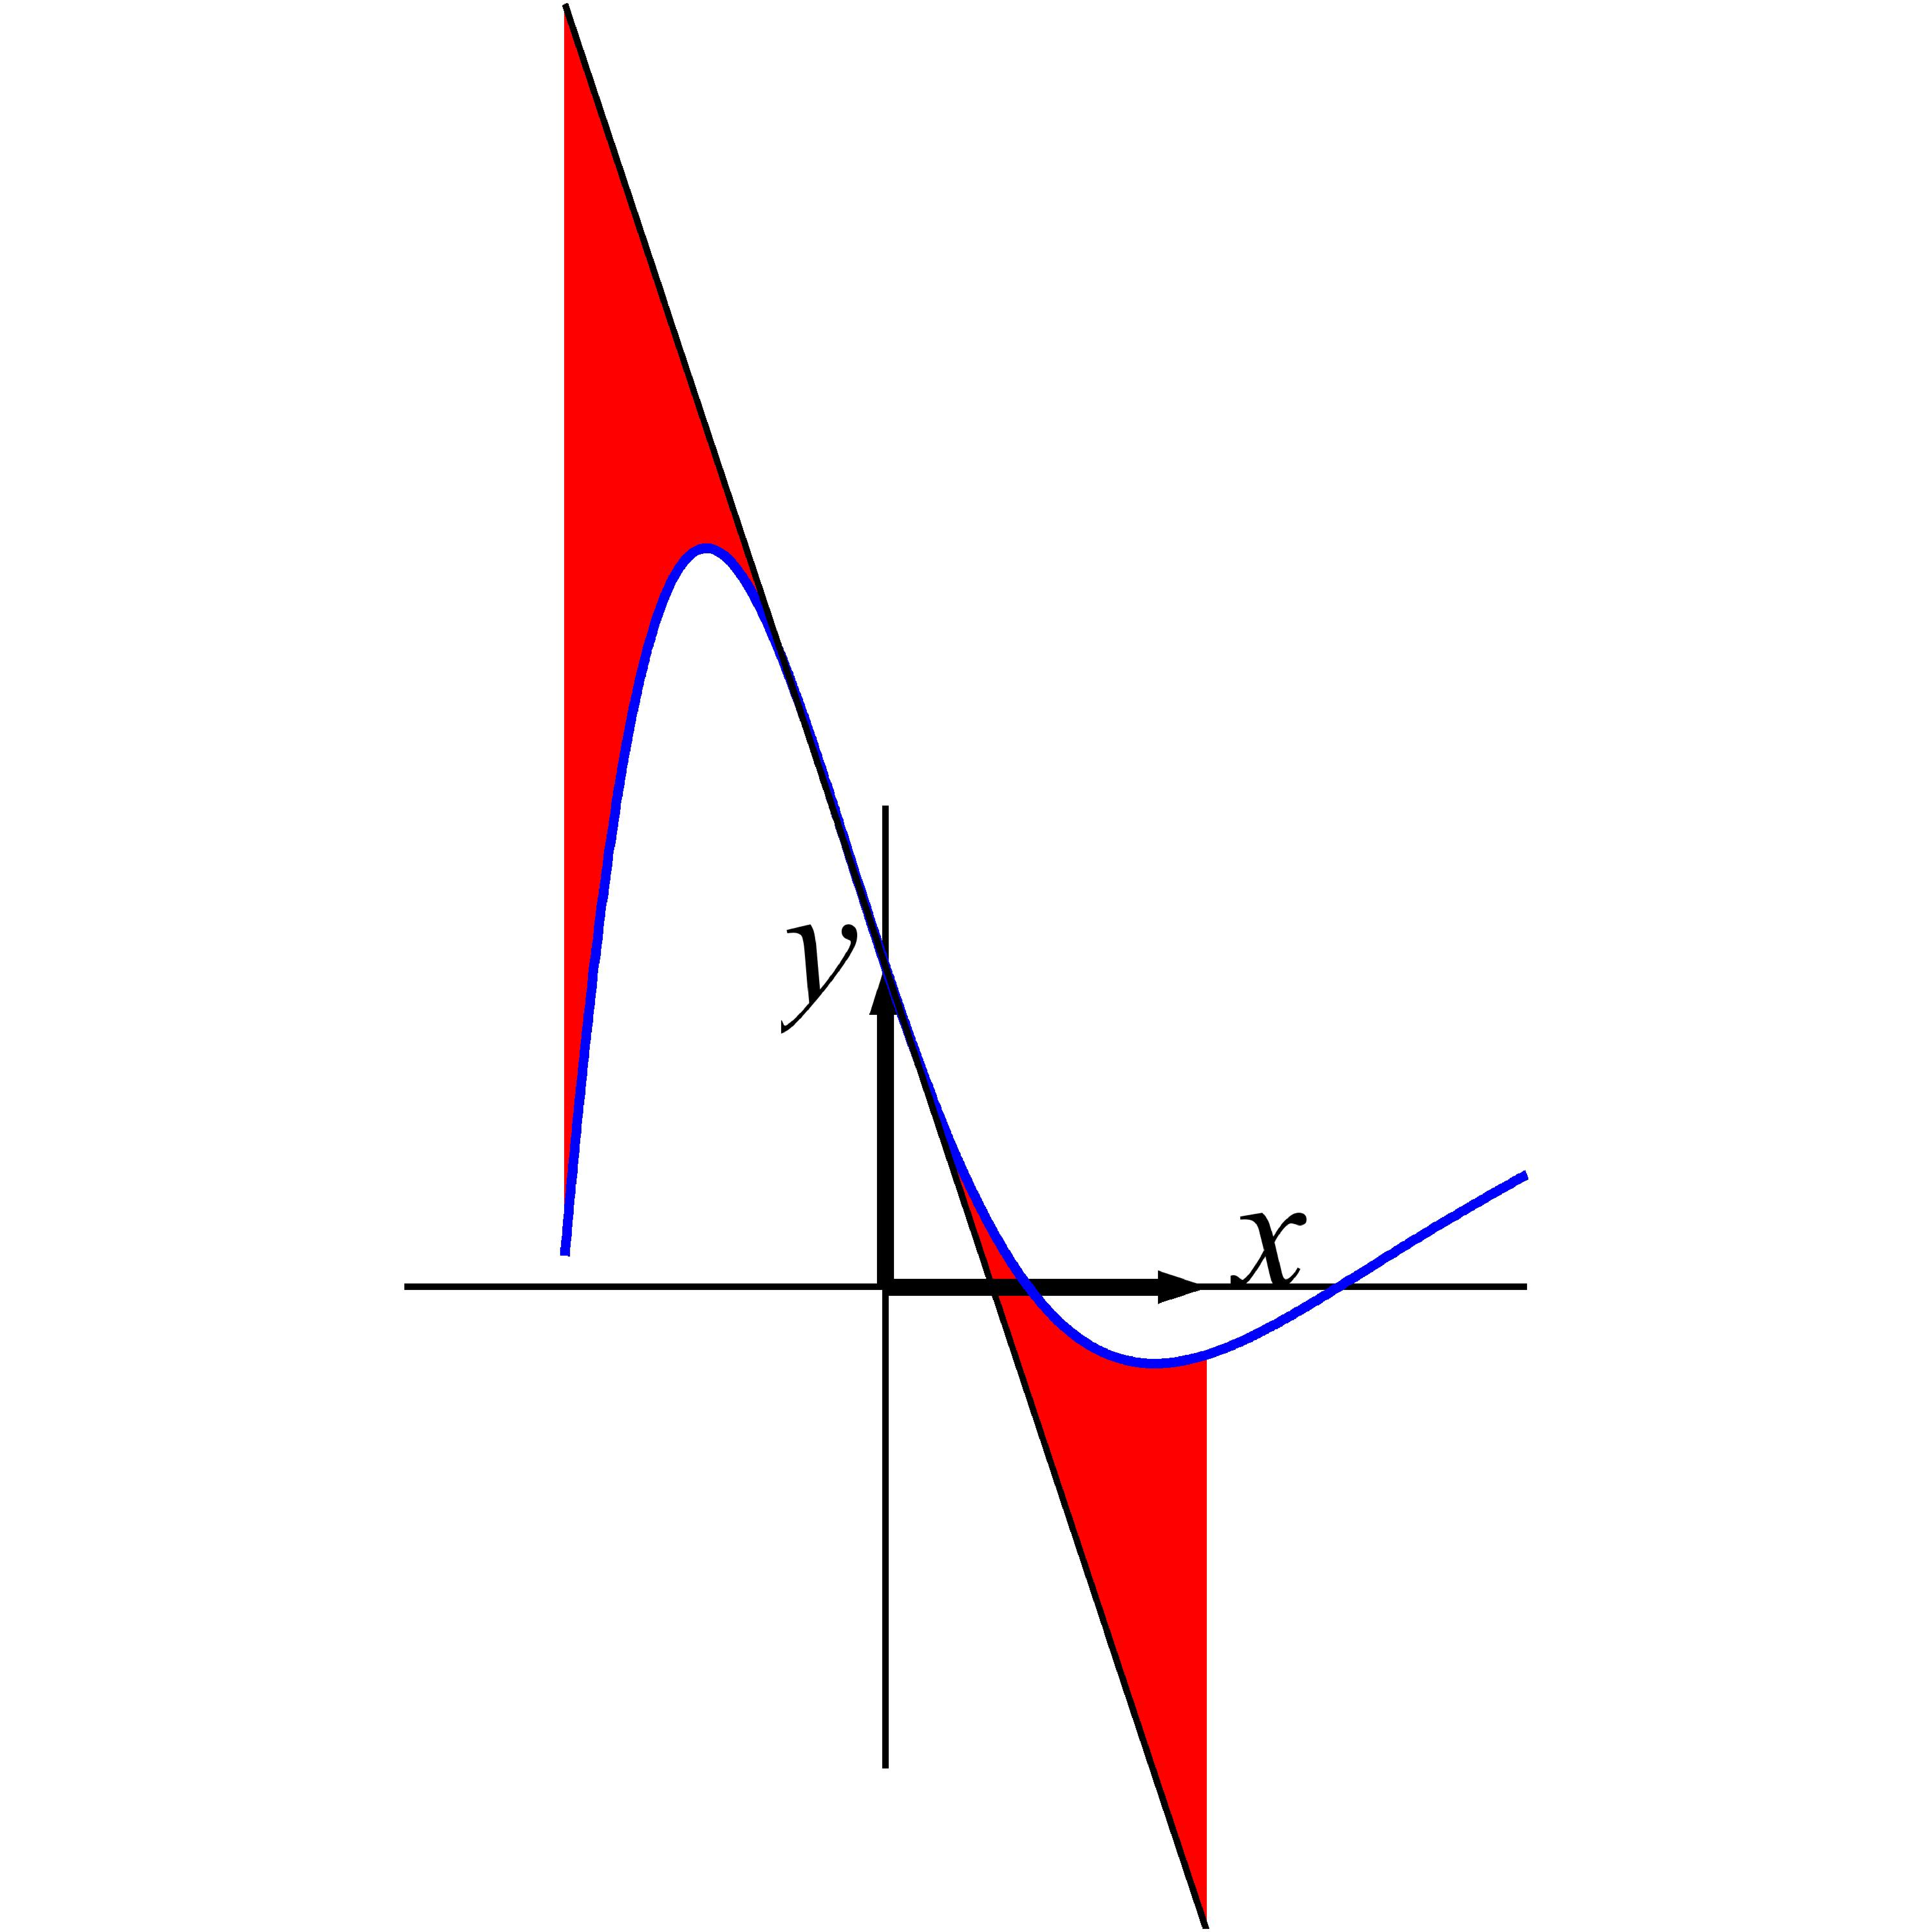
\includegraphics[height=55mm]{plotAp1.pdf} 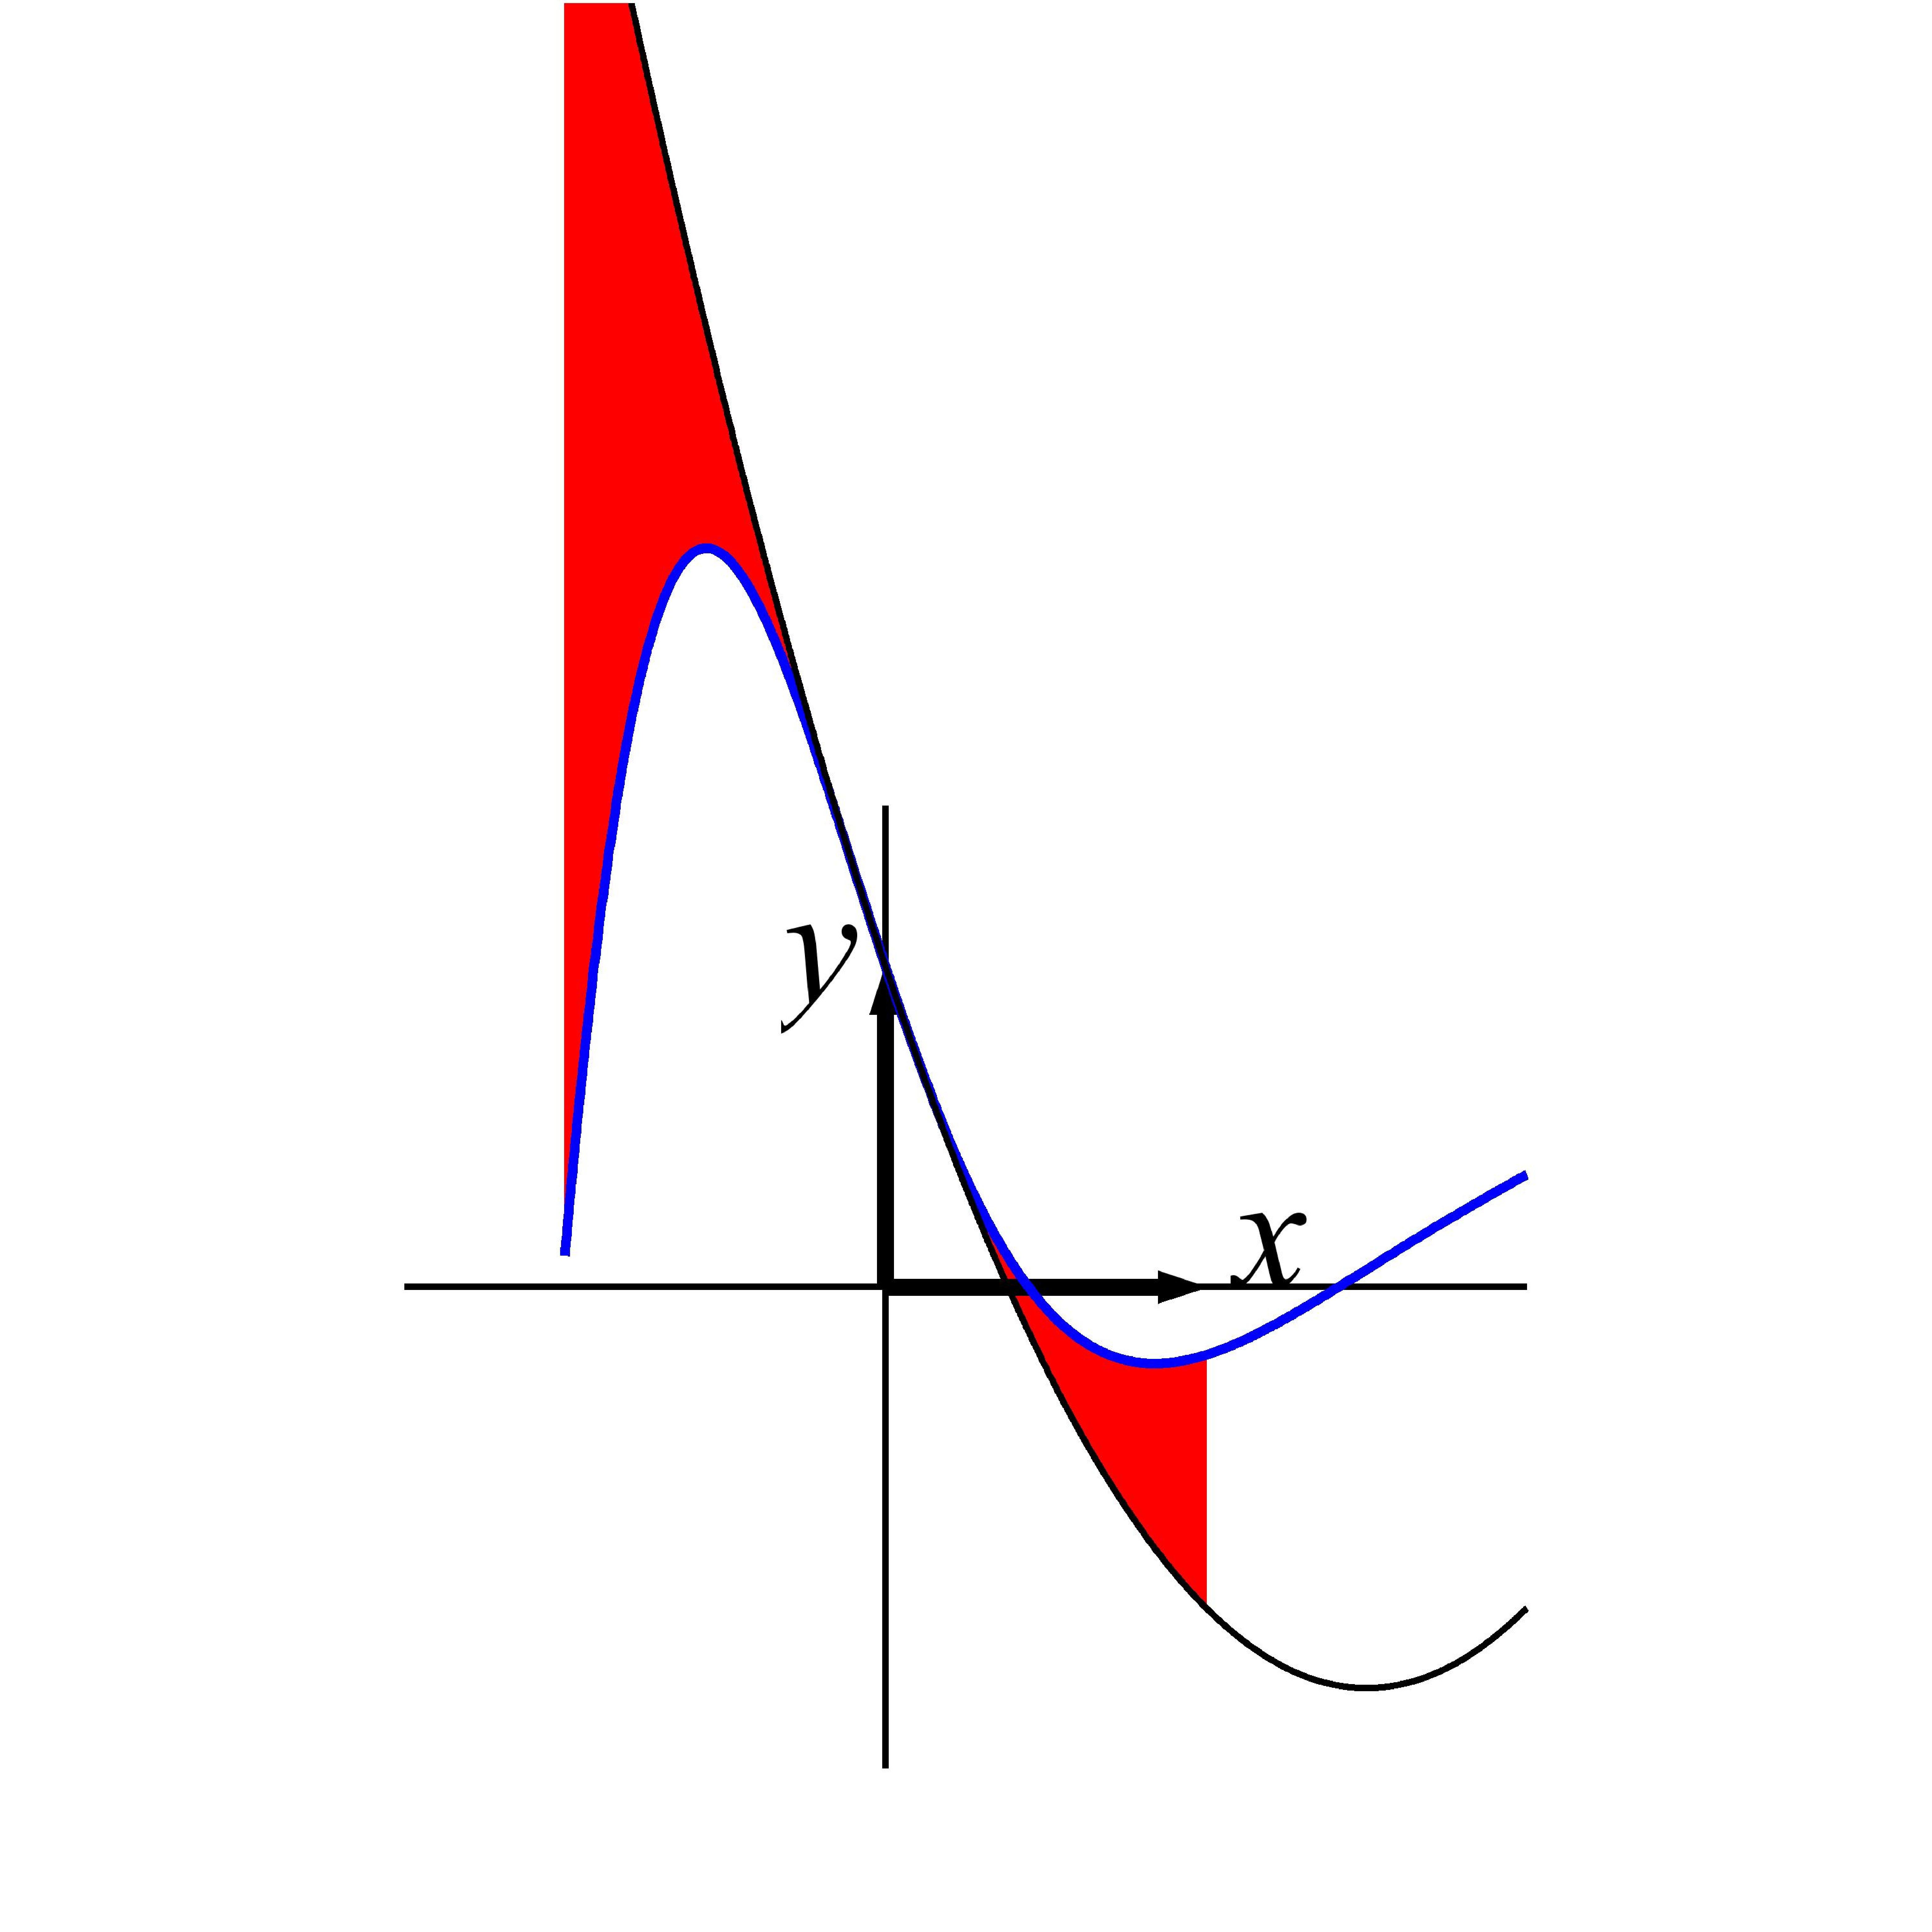
\includegraphics[height=55mm]{plotAp2.pdf} 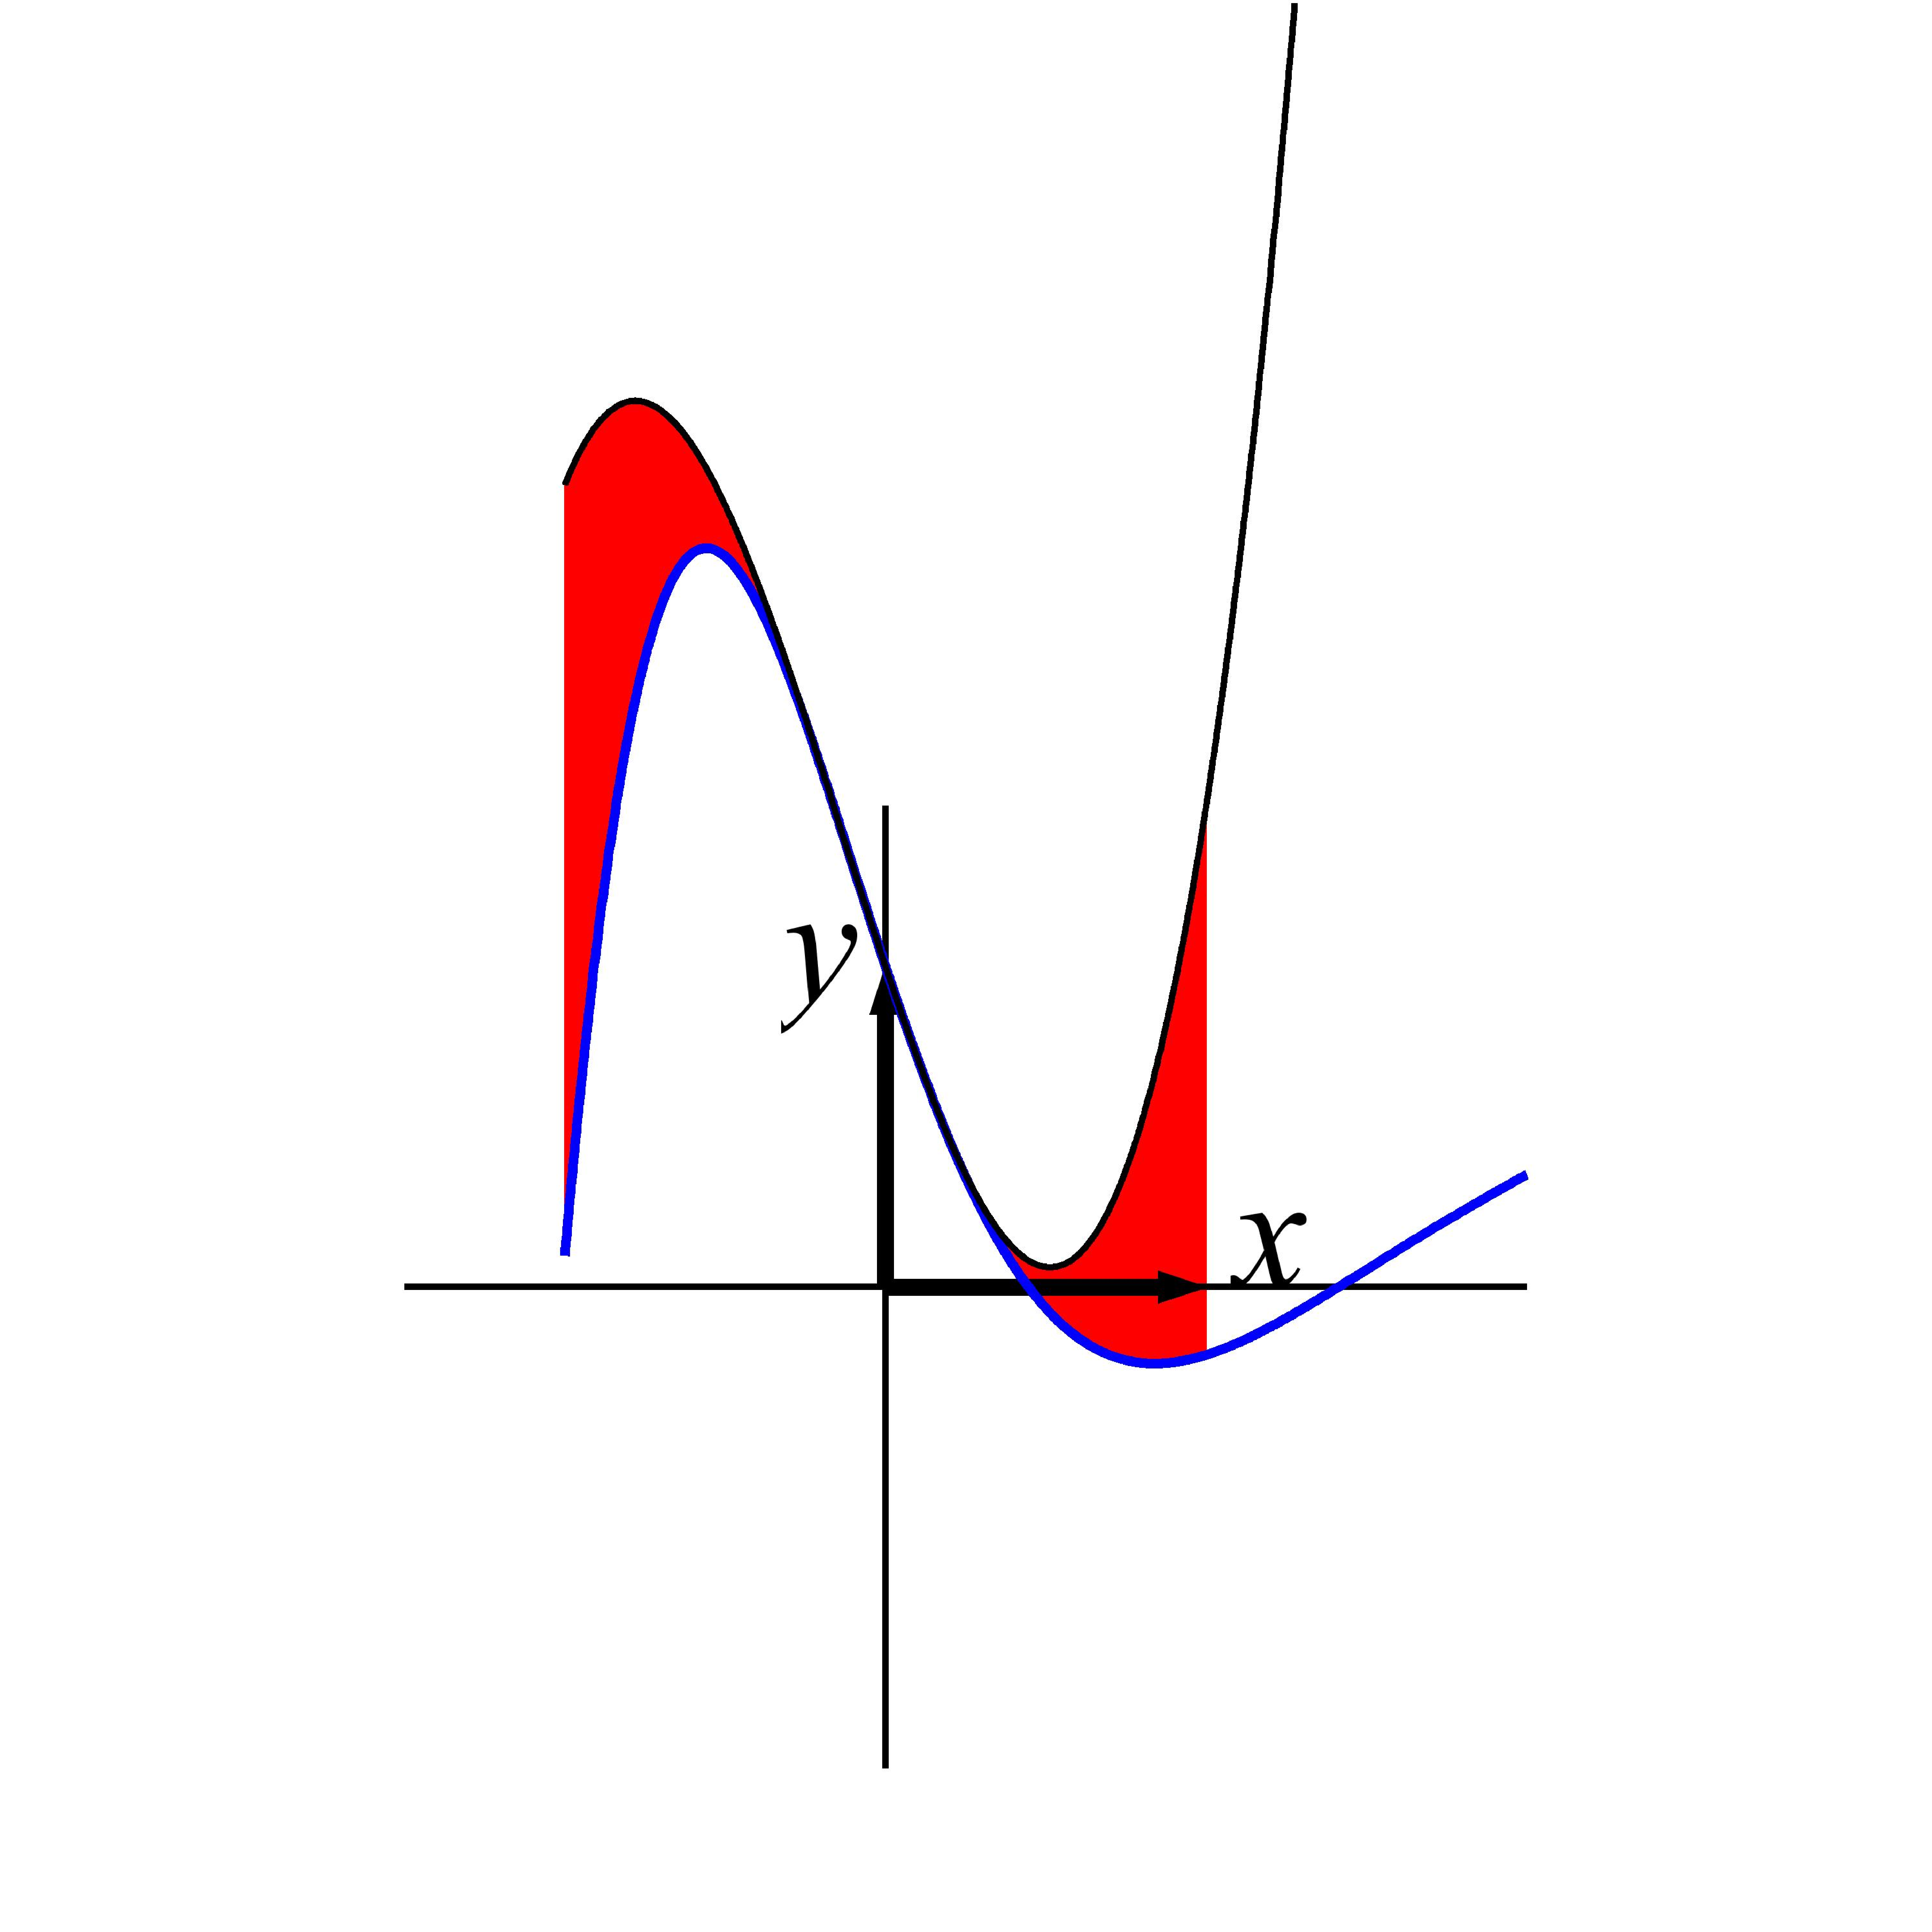
\includegraphics[height=55mm]{plotAp3.pdf}   }
\begin{center}
\caption{Funktionen $f(x)$ fra eksempel \ref{exampRestVurdering2} (blå) og de approksimerende første-, anden-, og tredjegrads-polynomier (sorte) med udviklingspunkt $x_{0}=0$. De tilhørende respektive restfunktioner (røde) er illustreret som forskellene mellem $f(x)$ og de approksimerende polynomier.} \label{figAp3}
\end{center}
\end{figure}




\begin{example}[Approksimation af ukendt (men elementær) funktion] \label{exampRestVurdering2}
Givet funktionen fra eksempel \ref{exampElemDiff}, dvs. funktionen tilfredsstiller følgende differentialligning med begyndelsesbetingelser:
\begin{equation} \label{eqDiffLignBeg}
f''(x) + 3f'(x) + 7f(x) = x^{2} \quad , \quad \textrm{hvor} \quad f(0) = 1 \quad , \quad \textrm{og} \quad f'(0) = -3 \quad,
\end{equation}
hvor vi har antaget, at højresiden i ligningen er $q(x)=x^{2}$ og at udviklingspunktet er $x_{0}=0$. Derved får vi nu:
\begin{equation}
f'(0) = -3 \quad , \quad  f''(0)= 2 \quad , \quad  f'''(0)= 15 \quad .
\end{equation}
Vi har
\begin{equation}
\begin{aligned}
f(x) &= f(0) + f'(0)\cdot x + \frac{f''(0)}{2}\cdot x^2 +  \frac{f'''(0)}{6}\cdot x^3 + x^{3}\cdot \varepsilon(x) \\
=& 1 - 3\cdot x + x^{2} +  \frac{5}{2}\cdot x^{3} + x^{3}\cdot \varepsilon(x) \quad,
\end{aligned}
\end{equation}
således at det approksimerende tredjegrads-polynomium for $f(x)$ med udviklingspunkt $x_{0}=0$ er
\begin{equation}
P_{3, x_{0}=0}(x) = 1 - 3\cdot x + x^{2} +  \frac{5}{2}\cdot x^{3} \quad.
\end{equation}
Bemærk, at $P_{3, x_{0}=0}(x)$ tilfredsstiller begyndelsesbetingelserne i (\ref{eqDiffLignBeg}) men polynomiet $P_{3, x_{0}=0}(x)$ er ikke en løsning til selve differentialligningen!
\end{example}




\section{Funktionsundersøgelser} \label{secFunkUnders}

En meget vigtig egenskab ved kontinuerte funktioner er følgende, som betyder at der er styr på hvor store og små værdier en kontinuert funktion kan antage på et interval, når blot
intervallet er tilstrækkelig pæn:

\begin{theorem}[Hovedsætning for kontinuerte funktioner af \'{e}n variabel] \label{thmHovedsaetnKontEn}
Lad $f(x)$ betegne en funktion som er kontinuert i hele sin definitionsmængde $\mathcal{D}m(f) \subset \mathbb{R}$.
Lad $I = [\, a \, , \, b \, ]$ være et begrænset, afsluttet, og sammenhængende interval i $\mathcal{D}m(f)$. \\

Så er værdimængden for funktionen $f(x)$ i intervallet $I$ også et
begrænset, afsluttet, og sammenhængende interval $[\, A \, , \, B \, ] \subset \mathbb{R}$. Vi kan skrive således:
\begin{equation}
\mathcal{V}m(f_{|_{I}}) = f(I) = \{ f(x)\, | \, x\in I \} =  [\, A \, , \, B \, ] \quad ,
\end{equation}
hvor der tillades den mulighed at $A = B$ og det sker jo præcis når $f(x)$ er konstant i hele intervallet $I$.
\end{theorem}

\begin{definition} [Globalt minimum og globalt maksimum]
Når en funktion $f(x)$ har værdimængden $\mathcal{V}m(f_{|_{I}}) = f(I) = [\, A \, , \, B \, ]$ på et interval $I = [a, b]$ siger vi, at
\begin{enumerate}
\item $A$ er den \ind{globale minimumværdi}{globale minimumværdi} for $f(x)$ i $I$, og hvis $f(x_{0})= A$ for $x_{0} \in I$ så er $x_{0}$ et \ind{globalt minimumpunkt}{globalt minimumpunkt} for $f(x)$ i $I$.
\item $B$ er den \ind{globale maksimumværdi}{globale maksimumværdi} for $f(x)$ i $I$, og hvis $f(x_{0})= B$ for $x_{0} \in I$ så er $x_{0}$ et \ind{globalt maksimumpunkt}{globalt maksimumpunkt} for $f(x)$ i $I$.
\end{enumerate}
\end{definition}

En velkendt og vigtig opgave går ud på at finde de globale maksimum- og minimum-værdier for givne funktioner $f(x)$ i givne intervaller og at bestemme de $x$-værdier for hvilke
disse maksimum- og minimum-værdier {\emph{antages}} altså minimum- og maksimum-punkterne. For at løse den opgave er følgende en uvurderlig hjælp -- se figur \ref{figVm}:

\begin{lemma}[Maksima og minima i stationære punkter]
Lad $x_{0}$ være en global maksimum- eller minimum-værdi for $f(x)$ i $I$. Antag, at  $x_{0}$ ikke er et endepunkt for intervallet $I$ og at $f(x)$ er differentiabel i $x_{0}$.\\
 Så er
$x_{0}$ et \ind{stationært punkt}{stationært punkt} for $f(x)$ i betydningen: $f'(x_{0}) = 0$.
\end{lemma}
\begin{bevis}
Vi antyder argumentet. Da $f(x)$ er antaget differentiabel, har vi:
\begin{equation}
\begin{aligned}
f(x) &= f(x_{0}) + f'(x_{0})\cdot(x-x_{0}) + (x-x_{0}) \cdot \varepsilon_{f}(x-x_{0}) \\
&= f(x_{0}) + (x- x_{0})\cdot(f'(x_{0}) + \varepsilon_{f}(x-x_{0})) \quad.
\end{aligned}
\end{equation}
Hvis vi nu antager, at $f'(x_{0})$ er positiv, så er parentesen $(f'(x_{0}) + \varepsilon_{f}(x-x_{0}))$ også positiv for $x$ tilstrækkelig tæt på $x_{0}$ (idet  $\varepsilon_{f}(x-x_{0}) \to 0$ for $x \to x_{0}$), men så er $(x- x_{0})\cdot(f'(x_{0}) + \varepsilon_{f}(x-x_{0}))$ også positiv for $x$ tilstrækkeligt tæt på $x_{0}$ og dermed er
$f(x) > f(x_{0})$ for sådanne $x > x_{0}$, og $f(x) < f(x_{0})$ for sådanne $x < x_{0}$. Derfor kan $f(x_{0})$ ikke være hverken maksimum-værdi eller minimumværdi for $f(x)$. Tilsvarende konklusion fås med antagelsen $f'(x_{0}) < 0 $. Hvis $x_{0}$ er en global maksimum- eller minimum-værdi for $f(x)$ i $I$ må den antagelse derfor medføre, at $f'(x_{0}) = 0$.
\end{bevis}

Hermed har vi følgende undersøgelsesmetode til rådighed:

\begin{method}[Undersøgelsesmetode]\label{metodeVm}
Lad $f(x)$ være en kontinuert funktion og $I = [a, b]$ et interval i definitionsmængden $\mathcal{D}m(f)$.\\

Maksimum- og minimum-værdierne for funktionen $f(x)$, $x \in I$, altså $A$ og $B$ i værdimængden $[A, B]$ for $f(x)$ i $I$  findes ved at finde og sammenligne funktionsværdierne i følgende punkter:
\begin{enumerate}
\item Interval-endepunkterne (randpunkterne $a$ og $b$ for intervallet $I$).
\item Undtagelsespunkter, dvs. de punkter i det åbne interval $]a, b[$ hvor funktionen {\emph{ikke}} er differentiabel.
\item De stationære punkter, dvs. samtlige de punkter $x_{0}$ i det åbne interval $]a, b[$  hvor $f'(x_{0}) = 0$.
\end{enumerate}
\end{method}

\begin{think}
Ved denne undersøgelsesmetode findes naturligvis ikke blot de globale maksimum- og minimum-værdier men også de $x$-værdier i $I$ for hvilke
det globale maksimum og det globale minimum antages, altså maksimum- og minimum-punkterne i det aktuelle interval.
\end{think}


\begin{example}[En kontinuert funktion undersøges] \label{exampKontFunk}
En kontinuert funktion $f(x)$ er defineret for alle $x$ på følgende måde:
\begin{equation}
f(x) = \left\{
        \begin{array}{ll}
         0.75 \, \,  & \hbox{for} \quad x \leq -1.5 \\
           0.5 + (x+1)^{2} \, \,  & \hbox{for} \quad -1.5 \leq x \leq 0  \\
           1.5\cdot(1-x^{3}) \, \,  & \hbox{for} \quad 0 \leq x \leq 1  \\
              x-1 \, \,  & \hbox{for} \quad 1 \leq x \leq 2  \\
          1 \, \, & \hbox{for} \quad x > 2
        \end{array}
      \right.
\end{equation}
Se figur \ref{figVm}, hvor vi kun betragter funktionen i intervallet $I = [-1.5, 2.0]$.
Der er to undtagelspunkter, hvor funktionen ikke er differentiabel: $x_{0}=0$ og $x_{0}=1$.
Der er \'{e}t stationært punkt i $]-1.5, 2.0[$ hvor $f'(x_{0}) = 0$ nemlig $x_{0}= -1$.
Og endelig er der de to randpunkter, intervalendepunkterne $x_{0}=-1.5$ og $x_{0}=2$ som skal undersøges.\\

Vi har derfor følgende kandidater til globale maksimum- og minimumværdier for $f(x)$ i $I$:
\begin{equation}
\begin{array}{|r|c|c|c|c|c|}
  \hline
  % after \\: \hline or \cline{col1-col2} \cline{col3-col4} ...
  x_{0} =  & -1.5 & -1 & 0 & 1 & 2\\ \hline
  f(x_{0}) =  & 0.75 & 0.5 & 1.5 & 0 & 1 \\
  \hline
\end{array}
\end{equation}
Vi aflæser konkluderende heraf, at maksimumværdien for $f(x)$ er $B = 1.5$ som antages i maksimumpunktet $x_{0} =0$. Minimumværdien er $A = 0$ som antages i minimumpunktet $x_{0}= 1$. Der er ikke andre maksimum- og minimum-punkter for $f(x)$ i $I$.
\end{example}



\begin{figure}[ht]
\centerline{ 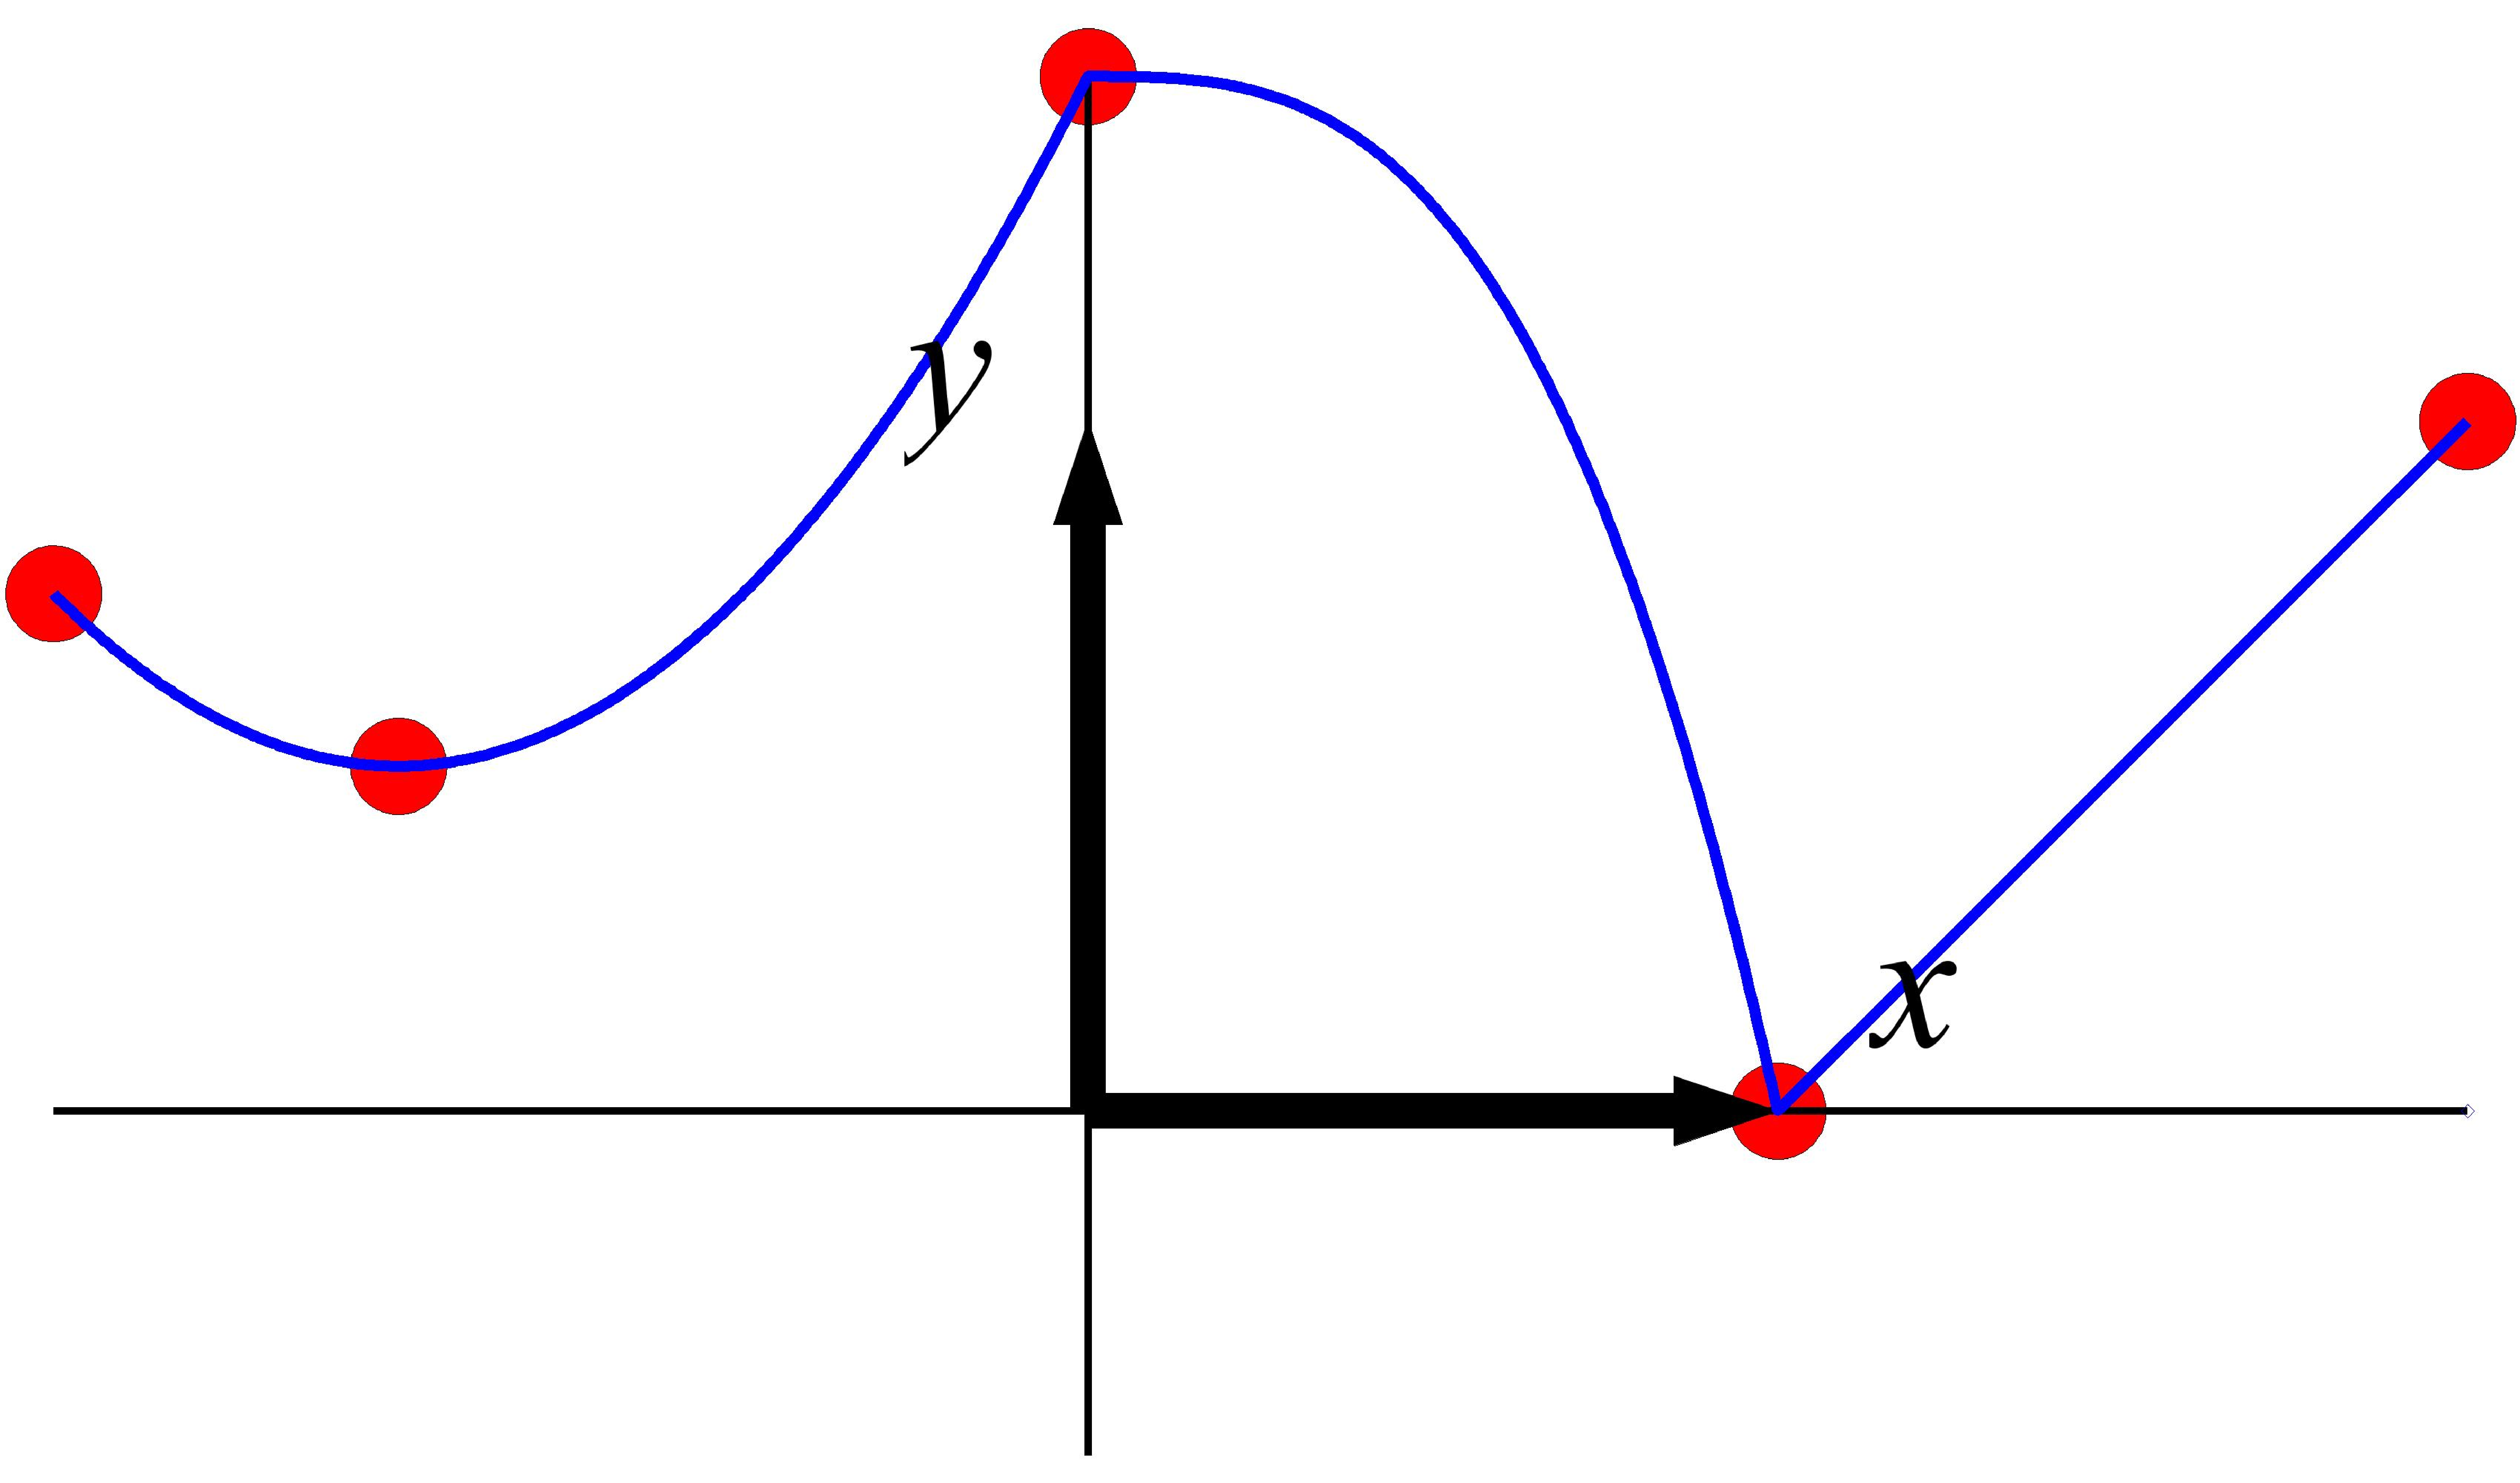
\includegraphics[height=45mm]{plotVm.pdf}}
\begin{center}
\caption{Den kontinuerte funktion $f(x)$ fra eksempel \ref{exampKontFunk} (blå). På grafen er markeret (med rødt) de $5$ punkter som skal undersøges specielt med henblik på at bestemme værdimængden for $f(x)$ i intervallet $[-1.5, 2]$, jvf. metode \ref{metodeVm}. } \label{figVm}
\end{center}
\end{figure}

\begin{definition}[Lokale minima og lokale maksima]
Lad $f(x)$ betegne en funktion på et interval $I = [a, b]$ som indeholder et givet $x_{0} \in ]a, b[$.
\begin{enumerate}
\item  Hvis $f(x) \geq f(x_{0})$ for alle $x$ i en (gerne lille) omegn om $x_{0}$, så kaldes $f(x_{0})$ en  \ind{lokal minimumværdi}{lokal minimumværdi} for $f(x)$ i $I$, og $x_{0}$ er et \ind{lokalt minimumpunkt}{lokalt minimumpunkt} for $f(x)$ i $I$. Hvis der faktisk gælder $f(x) > f(x_{0})$ for alle $x$ i omegnen fraregnet $x_{0}$ selv, så kaldes $f(x_{0})$ en \ind{egentlig lokal minimumværdi}{egentlig lokal minimumværdi}.
\item Hvis $f(x) \leq f(x_{0})$ for alle $x$ i en (gerne lille) omegn om $x_{0}$, så kaldes $f(x_{0})$ en  \ind{lokal maksimumværdi}{lokal maksimumværdi} for $f(x)$ i $I$, og $x_{0}$ er et \ind{lokalt maksimumpunkt}{lokalt maksimumpunkt} for $f(x)$ i $I$. Hvis der faktisk gælder $f(x) < f(x_{0})$ for alle $x$ i omegnen (fraregnet $x_{0}$ selv), så kaldes $f(x_{0})$ en \ind{egentlig lokal maksimumværdi}{egentlig lokal maksimumværdi}.
\end{enumerate}
\end{definition}

Hvis den funktion vi vil undersøge er glat i sine stationære punkter, så kan vi kvalificere metoden \ref{metodeVm} endnu bedre, idet det approksimerende polynomium af grad $2$ med udviklingspunkt i det stationære punkt kan hjælpe med at afgøre, om værdien af $f(x)$ i det stationære punkt er en kandidat til at være en maksimumværdi eller minimumværdi.

\begin{lemma}[Lokal analyse i et stationært punkt] \label{lemmaEkstrema}
Lad $f(x)$ være en glat funktion og antag, at $x_{0}$ er et stationært punkt for $f(x)$ i et interval $I = ]a, b[$.
Så gælder følgende:
\begin{enumerate}
\item Hvis $f''(x_{0}) > 0$ så er  $f(x_{0})$ en egentlig lokal minimumværdi for $f(x)$.
\item Hvis $f''(x_{0}) < 0$ så er $f(x_{0})$ en egentlig lokal maksimumværdi for $f(x)$.
\item Hvis $f''(x_{0}) = 0$ så er dette ikke tilstrækkelig information til at sikre, at $f(x_{0})$ er lokal minimumværdi eller lokal maksimumværdi.
\end{enumerate}
\end{lemma}

\begin{exercise}
Bevis hjælpesætningen \ref{lemmaEkstrema} ved at bruge Taylors grænseformel med det approksimerende andengrads-polynomium fro $f(x)$  og udviklingspunkt $x_{0}$. Husk, at $x_{0}$ er et stationært punkt, således at $f'(x_{0}) = 0$.
\end{exercise}


\begin{example}[Lokale maksima og minima] \label{exampLokMinMax}
Den kontinuerte funktionen $f(x)$
\begin{equation}
f(x) = \left\{
        \begin{array}{ll}
         0.75 \, \,  & \hbox{for} \quad x \leq -1.5 \\
           0.5 + (x+1)^{2} \, \,  & \hbox{for} \quad -1.5 \leq x \leq 0  \\
           1.5\cdot(1-x^{3}) \, \,  & \hbox{for} \quad 0 \leq x \leq 1  \\
              x-1 \, \,  & \hbox{for} \quad 1 \leq x \leq 2  \\
          1 \, \, & \hbox{for} \quad x \geq 2
        \end{array}
      \right.
\end{equation}
er vist i figur \ref{figVm}. I intervallet $I = [-1.5, 2.0]$ har funktionen de egentlige lokale minimumværdier $0.5$ og $0$
i de respektive egentlige lokale minimumpunkter $x_{0}= -1$ og $x_{0}= 1$ og funktionen har en egentlig lokal maksimumværdi $1.5$ i det egentlige lokale maksimumpunkt $x_{0}=0$. Hvis vi udvider intervallet til $J = [-7, 7]$ og bemærker at funktionsværdierne per definition er konstante udenfor intervallet $I$ fås de nye lokale maksimum-værdier $0.75$ og $1$ for $f(x)$ i $J$ -- ingen af dem er {\emph{egentlige}} lokale maksimumværdier.  Alle $x_{0} \in ]-7, -1.5]$ og alle $x_{0} \in [2, 7[$ er
lokale maksimumpunkter for $f(x)$ i $J$ men ingen af dem er {\emph{egentlige}} lokale maksimumpunkter. Alle $x_{0}$ i det {\emph{åbne interval}} $x_{0} \in ]-7, -1.5[$ og alle $x_{0}$ i det {\emph{åbne interval}} $x_{0} \in ]2, 7[$ er iøvrigt også
lokale minimumpunkter for $f(x)$ i $J$ men ingen af dem er {\emph{egentlige}} lokale minimumpunkter.
\end{example}


\begin{figure}[ht]
\centerline{ \includegraphics[height=45mm]{plotFresnelC.pdf}}
\begin{center}
\caption{Egentlige lokale maksima og egentlige lokale minima for funktionen fra eksempel \ref{exampFresnelC} er her antydet  på grafen for funktionen. For en ordens skyld bemærkes: De lokale maksimum- og minimum-punkter for funktionen er de markerede røde graf-punkters $x$-koordinater og de lokale maksimum- og minimum-værdier for funktionen er de markerede røde graf-punkters $y$-koordinater.} \label{figFresnelC}
\end{center}
\end{figure}

\begin{figure}[ht]
\centerline{ \includegraphics[height=45mm]{plotFresnelCPar.pdf}}
\begin{center}
\caption{Grafen for funktionen i eksempel \ref{exampFresnelC} og to approksimerende parabler med udviklingspunkter i to stationære punkter, som er henholdsvis et egentligt lokalt minimumpunkt og et egentligt lokalt maksimumpunkt for $f(x)$.} \label{figFresnelCPar}
\end{center}
\end{figure}

\begin{example}[En ikke-elementær funktion] \label{exampFresnelC}
Funktionen $f(x)$
\begin{equation}
f(x) = \int_{0}^{x}\, \cos(t^{2}) \, dt
\end{equation}
har stationære punkter i de værdier af $x_{0}$ som tilfredsstiller:
\begin{equation}
f'(x_{0}) = \cos(x_{0}^{2}) = 0 \quad , \quad \textrm{dvs.} \quad x_{0}^{2} = \frac{\pi}{2} + p\cdot \pi \quad \textrm{hvor $p$ er et helt tal} \quad.
\end{equation}
Da vi også har, at
\begin{equation}
f''(x) = -2\cdot x \cdot \sin(x^{2}) \quad ,
\end{equation}
sådan at der i de angivne stationære punkter gælder
\begin{equation}
f''(x_{0}) = -2 \cdot x_{0} \cdot (-1)^{p} \quad .
\end{equation}
Heraf følger -- via lemma \ref{lemmaEkstrema} -- at hvert andet stationært punkt $x_{0}$ langs $x$-aksen er et egentligt lokalt maksimumpunkt for $f(x)$ og de øvrige stationære
punkter er egentlige lokale minimumpunkter. Se figur \ref{figFresnelC}. I figur \ref{figFresnelCPar} er vist graferne (parabler) for et par af de approksimerende andengradspolynomier for $f(x)$ med udviklingspunkter i udvalgte stationære punkter.
\end{example}

\begin{example}[Når approksimation til grad $2$ ikke er nok] \label{exampStatPotens}
Som angivet i hjælpesætning \ref{lemmaEkstrema} kan man ikke ud fra $f'(x_{0}) = f''(x_{0}) = 0$ slutte, at funktionen har lokalt maksimum eller minimum i $x_{0}$. Det viser de tre simple funktioner i figur \ref{figStatPotens} med al ønskelig tydelighed: $f_{1}(x) = x^{4}$, $f_{2}(x) = - x^{4}$ og $f_{3}(x) = x^{3}$. Alle tre funktioner har stationært punkt i $x_{0}=0$ og alle har $f''(x_{0})=0$, men $f_{1}(x)$ har et egentligt lokalt minimumpunkt i $0$,  $f_{2}(x)$ har et egentligt lokalt maksimumpunkt i $0$, og $f_{3}(x)$ har hverken et lokalt minimimumpunkt eller et lokalt maksimumpunkt i $0$.
\end{example}

\begin{figure}[ht]
\centerline{ 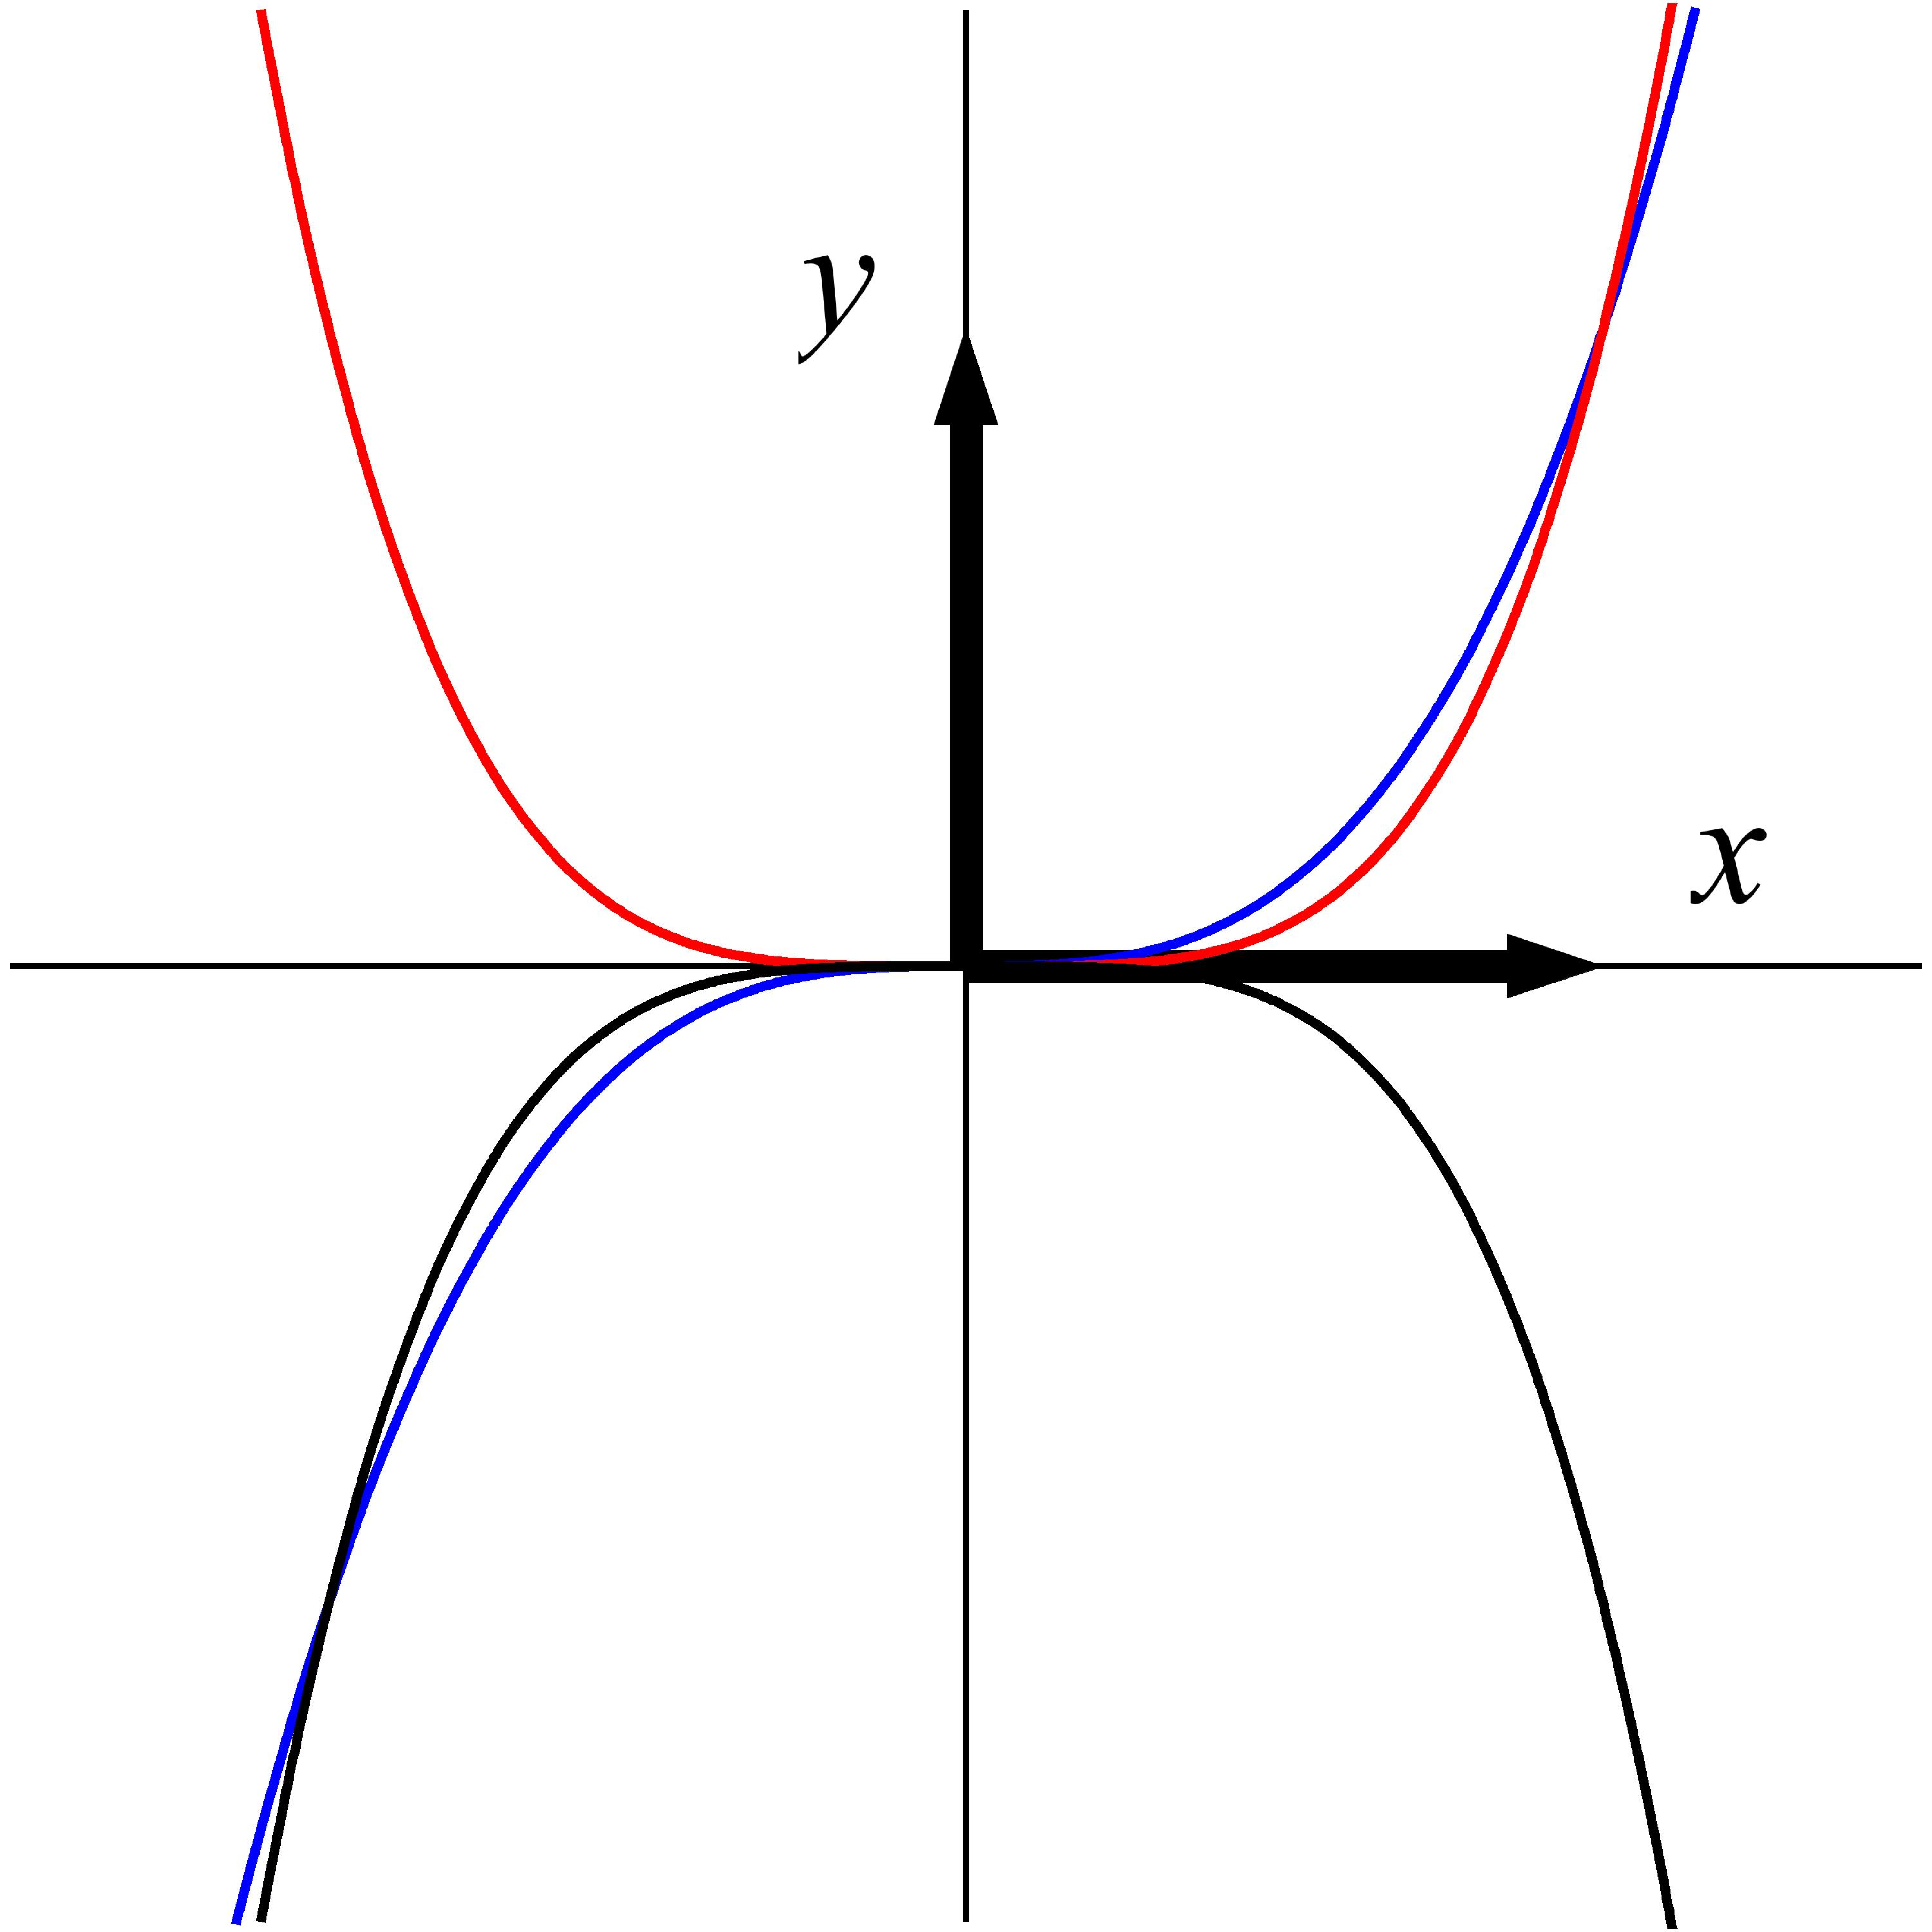
\includegraphics[height=55mm]{plotStatPotens.pdf}}
\begin{center}
\caption{Tre elementære funktioner med approksimerende andengrads-polynomium $P_{2, x_{0}=0}(x)=0$ for alle $x$. Funktionerne er henholdsvis: $f_{1}(x) = x^{4}$ (rød),  $f_{1}(x) = -x^{4}$ (sort), og $f_{3}(x) = x^{3}$ (blå).} \label{figStatPotens}
\end{center}
\end{figure}




%%%%%%%%%%%%%%%%%%%%%%%%%%%%%%%%%%%%%%%%%%%%%%%%%%%
%%%%%%%%%%%%%%%%%%%%%%%%%%%%%%%%%%%%%%%%%%%%%%%%%%%
%%%%%%%%%%%%%%%%%%%%%%%%%%%%%%%%%%%%%%%%%%%%%%%%%%%



\begin{summary}
I denne eNote har vi studeret hvordan man kan approksimere glatte funktioner med polynomier.
\begin{itemize}
\item Enhver glat funktion $f(x)$ på et interval $I$ kan opdeles i et approximerende $n$'te-grads-polynomium $P_{n, x_{0}}(x)$ med udviklingspunkt $x_{0}$ og en tilhørende restfunktion $R_{n, x_{0}}(x)$ således:
    \begin{equation}
  f(x) = P_{n, x_{0}}(x) + R_{n, x_{0}}(x) \quad ,
    \end{equation}
hvor polynomiet og restfunktionen i Taylor's grænseformel skrives således:
\begin{equation*}
f(x) = f(x_{0}) + \frac{f'(x_{0})}{1!}\cdot(x-x_{0}) + \cdots +
\frac{f^{(n)}(x_{0})}{n!}\cdot(x-x_{0})^{n} + (x-x_{0})^{n}\cdot\varepsilon_{f}(x-x_{0}) \quad ,
\end{equation*}
hvor $\varepsilon_{f}(x-x_{0})$ betegner en epsilonfunktion af $(x-x_{0})$, dvs. $\varepsilon_{f}(x-x_{0}) \to 0 $ for $x \to x_{0}$.
\item Taylor's grænseformel kan benyttes til at finde kontinuerte udvidelser af brøk\-funk\-tioner ved at finde (om muligt) deres grænseværdier for $x \to x_{0}$ hvor $x_{0}$ er de værdier hvor nævner-funktionen er $0$ således at brøkfunktionen i udgangspunktet ikke er defineret i $x_{0}$:
\begin{equation}
\frac{\sin(x)}{x} = \frac{x + x^{1}\cdot\varepsilon(x)}{x} = 1 + \varepsilon(x) \to 1 \quad \textrm{for} \quad x \to 0 \quad .
\end{equation}

\item Vurdering af restfunktionen giver en øvre grænse for den største numeriske forskel mellem en given funktion og det approksimerende polynomium af en  passende grad
og med et passende udviklingspunkt i et givet undersøgelsesinterval. En sådan vurdering  kan også foretages for funktioner, som måske kun ''kendes'' via en differentialligning eller som et ikke-elementært integral:
\begin{equation}
|\ln(x) - (x-1)| \leq \frac{1}{18} \quad \textrm{for alle} \quad x \in \left[\frac{3}{4}, \frac{5}{4} \right] \quad .
\end{equation}

\item Taylor's grænseformel med approksimerende anden-grads-polynomium
benyt\-tes til effektiv funktionsundersøgelse, herunder bestemmelse af værdimængde, globale og lokale maksima og minima for givne funktioner.
\end{itemize}
\end{summary}



%%%%%%%%%%%%%%%%%%%%%%%%%%%%%%%%%%%%%%%%%%%%%
%%%%%%%%%%%%%%%%%%%%%%%%%%%%%%%%%%%%%%%%%%%%%
%%% HER SKAL DU STOPPE MED AT SKRIVE %%%%%%%%
%%%%%%%%%%%%%%%%%%%%%%%%%%%%%%%%%%%%%%%%%%%%%
%%%%%%%%%%%%%%%%%%%%%%%%%%%%%%%%%%%%%%%%%%%%%


\end{document} 

%%%%%%%%%%%%%%%%%%%%%%%%%%%%%%%%%%%%%%%%%%%%%%%%%%%
%%%%%%%%%%%%%%%%%%%%%%%%%%%%%%%%%%%%%%%%%%%%%%%%%%% 